\documentclass[11pt,reqno]{amsart}
\usepackage{iftex}
\ifPDFTeX
  \usepackage[T1]{fontenc}
  \usepackage[utf8]{inputenc}
  \usepackage{lmodern}
\else
  \usepackage[no-math]{fontspec}
\fi
\usepackage{amsmath}
\usepackage{amssymb}
\usepackage{amsfonts}
\usepackage{mathrsfs}
\usepackage{amsthm}
\usepackage{mathtools}
\usepackage{geometry}
\usepackage{enumitem}
\usepackage{longtable}
\usepackage{booktabs}
\usepackage{array}
\usepackage{microtype}
\usepackage{graphicx}
\graphicspath{{../figures/}{figures/}}
\usepackage[dvipsnames]{xcolor}
\usepackage{float}
\usepackage{listings}
\lstset{basicstyle=\ttfamily\scriptsize,breaklines=true,columns=fullflexible,keepspaces=true,
  frame=single,framerule=0.3pt,showstringspaces=false,keywordstyle=\color{NavyBlue},
  commentstyle=\color{OliveGreen},stringstyle=\color{BrickRed},upquote=true}
\usepackage[pagebackref=true]{hyperref}
\usepackage{bookmark}
\usepackage{pdfcomment}

% Hover previews for internal references (no layout change).
\makeatletter
\let\CG@origref\ref
\let\CG@origeqref\eqref
\newcommand{\CG@gettip}[1]{\@ifundefined{CGTip@#1}{Reference: #1}{\csname CGTip@#1\endcsname}}
\DeclareRobustCommand{\CGref}[1]{\pdftooltip{\CG@origref{#1}}{\CG@gettip{#1}}}
\DeclareRobustCommand{\CGeqref}[1]{\pdftooltip{\CG@origeqref{#1}}{\CG@gettip{#1}}}
\makeatother
% Tooltip texts shown when hovering over internal references.
\makeatletter
\expandafter\gdef\csname CGTip@sec:introduction\endcsname{Section 1: Introduction (p. 2)}
\expandafter\gdef\csname CGTip@subsec:object\endcsname{Section 1.1: The object (p. 2)}
\expandafter\gdef\csname CGTip@eq:intro_zeta_euler\endcsname{Eq. (1.1), p. 2: zeta(s)=sum\_n=1\textasciicircum{}inf(1)/(n\textasciicircum{}s) =prod\_p prime(1-p\textasciicircum{}-s)\textasciicircum{}-1, Re s>1.}
\expandafter\gdef\csname CGTip@eq:intro_selberg_count\endcsname{Eq. (1.2), p. 3: N(T)=(T)/(2pi)log(T)/(2pi e)+(7)/(8) +(1)/(pi)arg zeta ((1)/(2)+iT) +O ((1)/(T)).}
\expandafter\gdef\csname CGTip@eq:intro_FL_equation\endcsname{Eq. (1.3), p. 3: (gamma)/(2pi)log(gamma)/(2pi e) +(1)/(pi)arg\textasciicircum{}*zeta ((1)/(2)+igamma) =conj k\_gamma-(11)/(8)+O ((1)/(gamma)).}
\expandafter\gdef\csname CGTip@eq:intro_clock\endcsname{Eq. (1.4), p. 3: tau\_k=(2pi (k-(11)/(8)))/(W\_0((k-(11)/(8))/e)) (k>=1).}
\expandafter\gdef\csname CGTip@eq:intro_defect\endcsname{Eq. (1.5), p. 3: u\_k(X)=k-(1)/(2)-N\_0(gamma\_k)-S\_X(gamma\_k),}
\expandafter\gdef\csname CGTip@subsec:main_results\endcsname{Section 1.2: Main results (p. 3)}
\expandafter\gdef\csname CGTip@eq:intro_main\endcsname{Eq. (1.6), p. 3: (1)/(no.I\_T)sum\_kin I\_Tu\_k(X)\textasciicircum{}2=(1)/(2pi\textasciicircum{}2)log(1)/(c)+O(1+sqrt(log(1/c))).}
\expandafter\gdef\csname CGTip@subsec:selberg_relation\endcsname{Section 1.3: Relation to Selberg's work (p. 4)}
\expandafter\gdef\csname CGTip@sec:notation\endcsname{Section 2: Notation and the clock (p. 4)}
\expandafter\gdef\csname CGTip@subsec:counting\endcsname{Section 2.1: Counting functions (p. 4)}
\expandafter\gdef\csname CGTip@eq:RvM\endcsname{Eq. (2.1), p. 4: N(t)=(1)/(pi)vartheta(t)+1+S(t), S(t)=(1)/(pi)arg zeta ((1)/(2)+it)=O(log t),}
\expandafter\gdef\csname CGTip@eq:N0_def\endcsname{Eq. (2.2), p. 4: Theta\_0(t)=(t)/(2)log(t)/(2pi e)-(pi)/(8), N\_0(t)=(1)/(pi)Theta\_0(t)+1, omega(t)=vartheta(t)-Theta\_0(t),}
\expandafter\gdef\csname CGTip@eq:N_decomposition\endcsname{Eq. (2.3), p. 4: N(t)=N\_0(t)+S(t)+(omega(t))/(pi) .}
\expandafter\gdef\csname CGTip@eq:L_def\endcsname{Eq. (2.4), p. 4: L(t)=N\_0'(t)=(1)/(2pi)log(t)/(2pi).}
\expandafter\gdef\csname CGTip@eq:IT_size\endcsname{Eq. (2.5), p. 4: no.I\_T=TL(T)+O(T).}
\expandafter\gdef\csname CGTip@subsec:clock\endcsname{Section 2.2: The clock and the displacements (p. 4)}
\expandafter\gdef\csname CGTip@lem:clock\endcsname{Lemma 2.1 (p. 4): The sequence (1.4) is the unique solution of N\_0(tau\_k)=k-(1)/(2) with tau\_k>2pi, k>=2. As a function of a real variable k, tau\_k is smooth and increasing with (dtau\_k)/(dk)=(1)/(L(tau\_k))=(2pi)/(log(tau\_k/2pi)).}
\expandafter\gdef\csname CGTip@eq:clock_derivative\endcsname{Eq. (2.6), p. 4: (dtau\_k)/(dk)=(1)/(L(tau\_k))=(2pi)/(log(tau\_k/2pi)).}
\expandafter\gdef\csname CGTip@def:displacements\endcsname{Definition 2.2 (p. 4): The ordinal displacement and the displacement of the clock are s\_k=k-(1)/(2)-N\_0(gamma\_k), delta\_k=tau\_k-gamma\_k .}
\expandafter\gdef\csname CGTip@eq:displacements\endcsname{Eq. (2.7), p. 4: s\_k=k-(1)/(2)-N\_0(gamma\_k), delta\_k=tau\_k-gamma\_k .}
\expandafter\gdef\csname CGTip@eq:s_delta\endcsname{Eq. (2.8), p. 4: s\_k=L(xi\_k) delta\_kfor some xi\_k between gamma\_k and tau\_k .}
\expandafter\gdef\csname CGTip@rem:gram_points\endcsname{Remark 2.3 (p. 4): Since Theta\_0(tau\_k)=pi(k-(3)/(2)) and vartheta=Theta\_0+omega, the clock point tau\_k is the point at which vartheta takes the value pi(k-(3)/(2)), up to a shift O(tau\_k\textasciicircum{}-1(log tau\_k)\textasciicircum{}-1). Thus tau\_k lies, in phase, half way between the Gram points g\_k-2 and g\_k-1, defined by vartheta(g\_n)=npi. The integer displaceme...}
\expandafter\gdef\csname CGTip@lem:s_bounds\endcsname{Lemma 2.4 (p. 5): For every k with gamma\_k>2, N(gamma\_k\textasciicircum{}-)-N\_0(gamma\_k)+(1)/(2)<= s\_k<= N(gamma\_k\textasciicircum{}+)-N\_0(gamma\_k)-(1)/(2), where N(gamma\textasciicircum{}+-) are the one-sided limits. In particular |s\_k|<=|S(gamma\_k\textasciicircum{}-)|+|S(gamma\_k\textasciicircum{}+)|+1.}
\expandafter\gdef\csname CGTip@eq:s_bounds\endcsname{Eq. (2.9), p. 5: N(gamma\_k\textasciicircum{}-)-N\_0(gamma\_k)+(1)/(2)<= s\_k<= N(gamma\_k\textasciicircum{}+)-N\_0(gamma\_k)-(1)/(2),}
\expandafter\gdef\csname CGTip@subsec:euler_phase\endcsname{Section 2.3: Euler phases and the truncated equation (p. 5)}
\expandafter\gdef\csname CGTip@eq:an_def\endcsname{Eq. (2.10), p. 5: a\_n=-(Lambda(n))/(pisqrt(n) log n),}
\expandafter\gdef\csname CGTip@eq:SA_def\endcsname{Eq. (2.11), p. 5: S\_A(t)=sum\_nin Aa\_nsin(tlog n), v\_A=(1)/(2)sum\_nin Aa\_n\textasciicircum{}2 .}
\expandafter\gdef\csname CGTip@eq:SX_def\endcsname{Eq. (2.12), p. 5: S\_X(t)=-(1)/(pi)sum\_p<= Xarg (1-p\textasciicircum{}-1/2-it)=-(1)/(pi)sum\_p<= Xsum\_m>=1(sin(mtlog p))/(m p\textasciicircum{}m/2),}
\expandafter\gdef\csname CGTip@eq:cP_def\endcsname{Eq. (2.13), p. 5: c\_P=(1)/(2pi\textasciicircum{}2)sum\_pin PLi\_2((1)/(p))=lim\_M->infv\_p\textasciicircum{}m: pin P, m<= M,}
\expandafter\gdef\csname CGTip@eq:sigma_M_def\endcsname{Eq. (2.14), p. 5: |S\_X(t)|<=sigma\_X:=(1)/(pi)sum\_p<= Xsum\_m>=1(1)/(m p\textasciicircum{}m/2), |S\_X'(t)|<= M\_X:=(1)/(pi)sum\_p<= X(log p)/(sqrt(p)-1),}
\expandafter\gdef\csname CGTip@def:LeClair_model\endcsname{Definition 2.5 (p. 5): For X>=2 the truncated counting model and the defect of the k-th zero are F\_X(t)=N\_0(t)+S\_X(t), u\_k(X)=k-(1)/(2)-F\_X(gamma\_k)=s\_k-S\_X(gamma\_k). The one-step corrected clock is tau\_k\textasciicircum{}X=tau\_k-(S\_X(tau\_k))/(L(tau\_k))=tau\_k-(dtau\_k)/(dk) S\_X(tau\_k), and, for a saturation level B>0, tau\_k\textasciicircum{}X,B=tau\_k-sat\_B(S\_X(tau\_k)/L(tau...}
\expandafter\gdef\csname CGTip@eq:defect_def\endcsname{Eq. (2.15), p. 5: F\_X(t)=N\_0(t)+S\_X(t), u\_k(X)=k-(1)/(2)-F\_X(gamma\_k)=s\_k-S\_X(gamma\_k).}
\expandafter\gdef\csname CGTip@eq:one_step_clock\endcsname{Eq. (2.16), p. 5: tau\_k\textasciicircum{}X=tau\_k-(S\_X(tau\_k))/(L(tau\_k))=tau\_k-(dtau\_k)/(dk) S\_X(tau\_k),}
\expandafter\gdef\csname CGTip@lem:LeClair_equation\endcsname{Lemma 2.6 (p. 5): The exact counting relation is N(t)=N\_0(t)+S(t)+omega(t)/pi, with omega(t)=O(1/t), as specified in (2.3). At a simple ordinate its midpoint value is N\_0(gamma\_k)+S\textasciicircum{}*(gamma\_k)+(omega(gamma\_k))/(pi) =k-(1)/(2). For a repeated ordinate the right side is conj k\_gamma-(1)/(2). Replacing S by S\_X and omitting the smooth r...}
\expandafter\gdef\csname CGTip@eq:exact_midpoint_ordinate\endcsname{Eq. (2.17), p. 5: N\_0(gamma\_k)+S\textasciicircum{}*(gamma\_k)+(omega(gamma\_k))/(pi) =k-(1)/(2).}
\expandafter\gdef\csname CGTip@sec:known_results\endcsname{Section 3: Known results used (p. 6)}
\expandafter\gdef\csname CGTip@thm:known_basic\endcsname{Theorem 3.1 (Riemann--von Mangoldt; Littlewood; [ref, Thms. 9.4, 9.9 and S 9.4], [ref]) (p. 6): S(t)=O(log t); the gaps gamma\_k+1-gamma\_k are bounded; and S\_1(t)=int\_0\textasciicircum{}tS(u) du=O(log t).}
\expandafter\gdef\csname CGTip@thm:known_BW\endcsname{Theorem 3.2 (Bellotti--Wong [ref]) (p. 6): For T>= e, |N(T)-(T)/(2pi)log(T)/(2pi e)|<=0.10076log T+0.24460log log T+8.08344 .}
\expandafter\gdef\csname CGTip@eq:BW_bound\endcsname{Eq. (3.1), p. 6: |N(T)-(T)/(2pi)log(T)/(2pi e)|<=0.10076log T+0.24460log log T+8.08344 .}
\expandafter\gdef\csname CGTip@thm:known_selberg_moments\endcsname{Theorem 3.3 (Selberg [ref]; see [ref, p. 225] and [ref, S 9.25]) (p. 6): For every integer j>=1, with c\_j=((2j)!)/(j! (2pi)\textasciicircum{}2j), int\_T\textasciicircum{}2TS(t)\textasciicircum{}2j dt=c\_j T(log log T)\textasciicircum{}j+O\_j(T(log log T)\textasciicircum{}j-1/2).}
\expandafter\gdef\csname CGTip@eq:selberg_moments\endcsname{Eq. (3.2), p. 6: int\_T\textasciicircum{}2TS(t)\textasciicircum{}2j dt=c\_j T(log log T)\textasciicircum{}j+O\_j(T(log log T)\textasciicircum{}j-1/2).}
\expandafter\gdef\csname CGTip@thm:known_selberg_approx\endcsname{Theorem 3.4 (Selberg's approximation, in the form of [ref, S 3, pp. 232--233]; [ref]) (p. 6): Let x\_0=T\textasciicircum{}1/160 and S\textasciicircum{}rm pr\_x\_0(t)=-(1)/(pi)sum\_p<x\_0p\textasciicircum{}-1/2sin(tlog p). Then int\_T\textasciicircum{}2T(S(t)-S\textasciicircum{}rm pr\_x\_0(t))\textasciicircum{}4dt<< T .}
\expandafter\gdef\csname CGTip@eq:selberg_approx\endcsname{Eq. (3.3), p. 6: int\_T\textasciicircum{}2T(S(t)-S\textasciicircum{}rm pr\_x\_0(t))\textasciicircum{}4dt<< T .}
\expandafter\gdef\csname CGTip@thm:known_MV\endcsname{Theorem 3.5 (Montgomery--Vaughan [ref, Cor. 3]) (p. 6): For complex b\_n, int\_T\textasciicircum{}2T|sum\_n<= Yb\_nn\textasciicircum{}-it|\textasciicircum{}2dt=sum\_n<= Y|b\_n|\textasciicircum{}2(T+O(n)) with an absolute implied constant.}
\expandafter\gdef\csname CGTip@thm:known_mertens\endcsname{Theorem 3.6 (Mertens [ref]) (p. 6): For y>=2, sum\_p<= y(log p)/(p)=log y+O(1) and sum\_p<= y(1)/(p)=log log y+B\_1+O((1)/(log y)) with a constant B\_1.}
\expandafter\gdef\csname CGTip@thm:known_KL\endcsname{Theorem 3.7 (Kusmin--Landau; [ref, Thm. 2.1]) (p. 6): Let f be real with a continuous monotone derivative on [a,b], and suppose that ||f'(x)||>=lambda>0 there, where ||*|| is the distance to the nearest integer. Then sum\_a<n<= be\textasciicircum{}2pi if(n)<<lambda\textasciicircum{}-1.}
\expandafter\gdef\csname CGTip@thm:known_landau\endcsname{Theorem 3.8 (Landau [ref]; uniform version by Gonek [ref]) (p. 6): For fixed x>1, sum\_0<gamma <= Tx\textasciicircum{}rho=-(T)/(2pi)Lambda(x)+O(log T), where Lambda(x)=0 unless x is a prime power, and the zeros are counted with multiplicity.}
\expandafter\gdef\csname CGTip@thm:known_RH_S\endcsname{Theorem 3.9 (Littlewood; [ref, Thm. 14.13]) (p. 6): On the Riemann hypothesis, S(t)=O(log t/log log t).}
\expandafter\gdef\csname CGTip@sec:identities\endcsname{Section 4: Exact identities at the zeros (p. 7)}
\expandafter\gdef\csname CGTip@thm:identity_general\endcsname{Theorem 4.1 (p. 7): Let m<n be indices, let F be a real C\textasciicircum{}1 function on [gamma\_m,gamma\_n] and put u\_k=k-(1)/(2)-F(gamma\_k) for m<= k<= n. For every integer j>=1, int\_gamma\_m\textasciicircum{}gamma\_n(N(t)-F(t))\textasciicircum{}2jF'(t) dt=sum\_k=m+1\textasciicircum{}n-1P\_j(u\_k)+(((1)/(2)+u\_m)\textasciicircum{}2j+1+((1)/(2)-u\_n)\textasciicircum{}2j+1)/(2j+1), where P\_j(u)=(((1)/(2)+u)\textasciicircum{}2j+1+((1)/(2)-u)\textasciicircum{}2j+1)/(2j+1)=sum\_i=0...}
\expandafter\gdef\csname CGTip@eq:identity_general\endcsname{Eq. (4.1), p. 7: int\_gamma\_m\textasciicircum{}gamma\_n(N(t)-F(t))\textasciicircum{}2jF'(t) dt=sum\_k=m+1\textasciicircum{}n-1P\_j(u\_k)+(((1)/(2)+u\_m)\textasciicircum{}2j+1+((1)/(2)-u\_n)\textasciicircum{}2j+1)/(2j+1),}
\expandafter\gdef\csname CGTip@eq:Pj_def\endcsname{Eq. (4.2), p. 7: P\_j(u)=(((1)/(2)+u)\textasciicircum{}2j+1+((1)/(2)-u)\textasciicircum{}2j+1)/(2j+1)=sum\_i=0\textasciicircum{}jbinom(2j+1,2i)(2\textasciicircum{}2i-2j)/(2j+1) u\textasciicircum{}2i=u\textasciicircum{}2j+sum\_i<jb\_j,iu\textasciicircum{}2i.}
\expandafter\gdef\csname CGTip@eq:identity_quadratic\endcsname{Eq. (4.3), p. 7: sum\_k=m+1\textasciicircum{}n-1u\_k\textasciicircum{}2=int\_gamma\_m\textasciicircum{}gamma\_n(N(t)-F(t))\textasciicircum{}2F'(t) dt-(n-m-1)/(12)-(((1)/(2)+u\_m)\textasciicircum{}3+((1)/(2)-u\_n)\textasciicircum{}3)/(3) .}
\expandafter\gdef\csname CGTip@eq:identity_one_gap\endcsname{Eq. (4.4), p. 7: int\_gamma\_k\textasciicircum{}gamma\_k+1(k-F(t))\textasciicircum{}2jF'(t) dt=int\_F(gamma\_k)\textasciicircum{}F(gamma\_k+1)(k-y)\textasciicircum{}2jdy=(((1)/(2)-u\_k+1)\textasciicircum{}2j+1+((1)/(2)+u\_k)\textasciicircum{}2j+1)/(2j+1),}
\expandafter\gdef\csname CGTip@rem:twelfth\endcsname{Remark 4.2 (p. 7): The constant (1)/(12) is the mean square of a centred sawtooth of unit step: between two consecutive zeros N-F decreases through one unit in the variable y=F(t). Identity (4.3) therefore says that the mean square of the defect at the zeros is the dF-mean square of N-F minus the contribution of the sawtooth. Nothing...}
\expandafter\gdef\csname CGTip@cor:identity_clock\endcsname{Corollary 4.3 (p. 7): With F=N\_0, so that u\_k=s\_k and N-N\_0=S+omega/pi almost everywhere, sum\_k=m+1\textasciicircum{}n-1s\_k\textasciicircum{}2=int\_gamma\_m\textasciicircum{}gamma\_n(S(t)+(omega(t))/(pi))\textasciicircum{}2L(t) dt-(n-m-1)/(12)-(((1)/(2)+s\_m)\textasciicircum{}3+((1)/(2)-s\_n)\textasciicircum{}3)/(3) . With F=F\_X, so that u\_k=u\_k(X) and N-F\_X=S-S\_X+omega/pi almost everywhere, sum\_k=m+1\textasciicircum{}n-1u\_k(X)\textasciicircum{}2=int\_gamma\_m\textasciicircum{}gamma\_n(S(t)-S\_X(...}
\expandafter\gdef\csname CGTip@eq:identity_clock\endcsname{Eq. (4.5), p. 7: sum\_k=m+1\textasciicircum{}n-1s\_k\textasciicircum{}2=int\_gamma\_m\textasciicircum{}gamma\_n(S(t)+(omega(t))/(pi))\textasciicircum{}2L(t) dt-(n-m-1)/(12)-(((1)/(2)+s\_m)\textasciicircum{}3+((1)/(2)-s\_n)\textasciicircum{}3)/(3) .}
\expandafter\gdef\csname CGTip@eq:identity_LeClair\endcsname{Eq. (4.6), p. 7: sum\_k=m+1\textasciicircum{}n-1u\_k(X)\textasciicircum{}2=int\_gamma\_m\textasciicircum{}gamma\_n(S(t)-S\_X(t)+(omega(t))/(pi))\textasciicircum{}2(L(t)+S\_X'(t))dt-(n-m-1)/(12)-(((1)/(2)+u\_m)\textasciicircum{}3+((1)/(2)-u\_n)\textasciicircum{}3)/(3) .}
\expandafter\gdef\csname CGTip@lem:first_moment_identity\endcsname{Lemma 4.4 (p. 8): Let 2<a<b be points which are not ordinates, let fin C\textasciicircum{}1[a,b] and G=N-N\_0. Then sum\_a<gamma\_k<= bs\_kf(gamma\_k)=int\_a\textasciicircum{}bG(t)f(t)L(t) dt+(1)/(2)[f G\textasciicircum{}2]\_a\textasciicircum{}b-(1)/(2)int\_a\textasciicircum{}bG(t)\textasciicircum{}2f'(t) dt .}
\expandafter\gdef\csname CGTip@eq:first_moment_identity\endcsname{Eq. (4.7), p. 8: sum\_a<gamma\_k<= bs\_kf(gamma\_k)=int\_a\textasciicircum{}bG(t)f(t)L(t) dt+(1)/(2)[f G\textasciicircum{}2]\_a\textasciicircum{}b-(1)/(2)int\_a\textasciicircum{}bG(t)\textasciicircum{}2f'(t) dt .}
\expandafter\gdef\csname CGTip@cor:cumulative\endcsname{Corollary 4.5 (p. 8): sum\_gamma\_k<= ts\_k=O(log\textasciicircum{}2t). In particular the mean of s\_k over k<= K is O(K\textasciicircum{}-1log\textasciicircum{}2K).}
\expandafter\gdef\csname CGTip@sec:clock_moments\endcsname{Section 5: Moments and extremes of the clock displacement (p. 8)}
\expandafter\gdef\csname CGTip@thm:clock_moments\endcsname{Theorem 5.1 (p. 8): For every fixed integer j>=1, as T->inf, (1)/(no.I\_T)sum\_kin I\_Ts\_k\textasciicircum{}2j=c\_j(log log T)\textasciicircum{}j+O\_j((log log T)\textasciicircum{}j-1/2), c\_j=((2j)!)/(j! (2pi)\textasciicircum{}2j) . In particular the mean square of s\_k over I\_T is (1)/(2pi\textasciicircum{}2)log log T+O(sqrt(log log T)) and (1)/(no.I\_T)sum\_kin I\_Tdelta\_k\textasciicircum{}2=(2log log T)/(log\textasciicircum{}2T)(1+O((log log T)\textasciicircum{}-1/2)).}
\expandafter\gdef\csname CGTip@eq:clock_moments\endcsname{Eq. (5.1), p. 8: (1)/(no.I\_T)sum\_kin I\_Ts\_k\textasciicircum{}2j=c\_j(log log T)\textasciicircum{}j+O\_j((log log T)\textasciicircum{}j-1/2), c\_j=((2j)!)/(j! (2pi)\textasciicircum{}2j) .}
\expandafter\gdef\csname CGTip@eq:delta_mean_square\endcsname{Eq. (5.2), p. 8: (1)/(no.I\_T)sum\_kin I\_Tdelta\_k\textasciicircum{}2=(2log log T)/(log\textasciicircum{}2T)(1+O((log log T)\textasciicircum{}-1/2)).}
\expandafter\gdef\csname CGTip@eq:moments_step1\endcsname{Eq. (5.3), p. 8: sum\_k=m+1\textasciicircum{}n-1P\_j(s\_k)=int\_gamma\_m\textasciicircum{}gamma\_n(S+(omega)/(pi))\textasciicircum{}2jL dt+O(log\textasciicircum{}2j+1T),}
\expandafter\gdef\csname CGTip@eq:moments_step2\endcsname{Eq. (5.4), p. 8: int\_T\textasciicircum{}2TS\textasciicircum{}2jL dt=L(T) c\_jT(log log T)\textasciicircum{}j+O(L(T) T(log log T)\textasciicircum{}j-1/2).}
\expandafter\gdef\csname CGTip@eq:moments_step3\endcsname{Eq. (5.5), p. 8: (1)/(no.I\_T)sum\_kin I\_TP\_j(s\_k)=c\_j(log log T)\textasciicircum{}j+O((log log T)\textasciicircum{}j-1/2).}
\expandafter\gdef\csname CGTip@cor:clock_distribution\endcsname{Corollary 5.2 (p. 9): Let sigma\_T\textasciicircum{}2=(1)/(2pi\textasciicircum{}2)log log T and let Z be a standard normal variable. For every fixed eta >=0, (1)/(no.I\_T)no.kin I\_T:|s\_k|<=eta sigma\_T-> P(|Z|<=eta). In particular, for every fixed A>0, no.kin I\_T:|s\_k|<= A=o(no.I\_T).}
\expandafter\gdef\csname CGTip@eq:clock_distribution\endcsname{Eq. (5.6), p. 9: (1)/(no.I\_T)no.kin I\_T:|s\_k|<=eta sigma\_T-> P(|Z|<=eta).}
\expandafter\gdef\csname CGTip@rem:korolev\endcsname{Remark 5.3 (p. 9): Selberg stated, and Korolev proved [ref], moment formulae for the integer displacement of gamma\_n with respect to the Gram intervals, and Korolev deduced that gamma\_n lies in its own Gram interval only for a set of indices of density zero. By Remark 2.3, Theorem 5.1 and Corollary 5.2 are the analogous statements for...}
\expandafter\gdef\csname CGTip@prop:extremes\endcsname{Proposition 5.4 (p. 9): item limsup\_k->infs\_k=+inf and liminf\_k->infs\_k=-inf. item limsup\_k->inf|delta\_k|<=2pi *0.10076=0.633093.... item On the Riemann hypothesis, delta\_k->0.}
\expandafter\gdef\csname CGTip@eq:sawtooth_sandwich\endcsname{Eq. (5.7), p. 9: s\_k+1-(1)/(2)<= N(t)-N\_0(t)<= s\_k+(1)/(2) .}
\expandafter\gdef\csname CGTip@eq:holder_contradiction\endcsname{Eq. (5.8), p. 9: int\_T\textasciicircum{}2TS\textasciicircum{}2dt<=(int\_T\textasciicircum{}2T|S| dt)\textasciicircum{}2/3(int\_T\textasciicircum{}2TS\textasciicircum{}4dt)\textasciicircum{}1/3<< T(log log T)\textasciicircum{}2/3,}
\expandafter\gdef\csname CGTip@prop:BW_pointwise\endcsname{Proposition 5.5 (Effective finite-height consequence of Bellotti--Wong) (p. 9): Let E(t)=0.10076log t+0.24460log log t+8.08344. For every k, -(E(gamma\_k)+3/8)/(L(tau\_k)) <=delta\_k<=(E(gamma\_k)-11/8)/(L(gamma\_k)). These inequalities are analytic and unconditional, and count repeated ordinates individually.}
\expandafter\gdef\csname CGTip@eq:BW_pointwise\endcsname{Eq. (5.9), p. 9: -(E(gamma\_k)+3/8)/(L(tau\_k)) <=delta\_k<=(E(gamma\_k)-11/8)/(L(gamma\_k)).}
\expandafter\gdef\csname CGTip@eq:BW_ordinal_sandwich\endcsname{Eq. (5.10), p. 10: -E(gamma\_k)-3/8<= s\_k<= E(gamma\_k)-11/8.}
\expandafter\gdef\csname CGTip@prop:fixed_sup\endcsname{Proposition 5.6 (p. 10): Let X>=2 be fixed and Bin(0,inf]. Then limsup\_k|delta\_k\textasciicircum{}X,B|=limsup\_k|delta\_k|, while limsup\_k|u\_k(X)|=inf.}
\expandafter\gdef\csname CGTip@sec:main_theorem\endcsname{Section 6: The main theorem: a variable cutoff in the truncated equation (p. 10)}
\expandafter\gdef\csname CGTip@subsec:main_statement\endcsname{Section 6.1: Statement (p. 10)}
\expandafter\gdef\csname CGTip@thm:main\endcsname{Theorem 6.1 (p. 10): There are absolute constants T\_0 and C such that for T>= T\_0 and every X with 2<= X<= T\textasciicircum{}1/2, writing c=log X/log T, |(1)/(no.I\_T)sum\_kin I\_Tu\_k(X)\textasciicircum{}2-(1)/(2pi\textasciicircum{}2)log(1)/(c)|<= C(1+sqrt(log(1/c))).}
\expandafter\gdef\csname CGTip@eq:main_theorem\endcsname{Eq. (6.1), p. 10: |(1)/(no.I\_T)sum\_kin I\_Tu\_k(X)\textasciicircum{}2-(1)/(2pi\textasciicircum{}2)log(1)/(c)|<= C(1+sqrt(log(1/c))).}
\expandafter\gdef\csname CGTip@cor:fixed_cutoff\endcsname{Corollary 6.2 (fixed cutoff) (p. 10): Let X>=2 be fixed. Then (1)/(no.I\_T)sum\_kin I\_Tu\_k(X)\textasciicircum{}2=(1)/(2pi\textasciicircum{}2)log log T+O\_X(sqrt(log log T)), and for every fixed A>0, no.kin I\_T:|u\_k(X)|<= A=o(no.I\_T).}
\expandafter\gdef\csname CGTip@eq:fixed_cutoff\endcsname{Eq. (6.2), p. 10: (1)/(no.I\_T)sum\_kin I\_Tu\_k(X)\textasciicircum{}2=(1)/(2pi\textasciicircum{}2)log log T+O\_X(sqrt(log log T)),}
\expandafter\gdef\csname CGTip@cor:power_cutoff\endcsname{Corollary 6.3 (power cutoff) (p. 10): Let 0<c<=(1)/(2) be fixed and X=T\textasciicircum{}c. Then limsup\_T->inf(1)/(no.I\_T)sum\_kin I\_Tu\_k(T\textasciicircum{}c)\textasciicircum{}2<=(1)/(2pi\textasciicircum{}2)log(1)/(c)+C(1+sqrt(log(1/c))), and for every function eta(T)->inf, no.kin I\_T:|u\_k(T\textasciicircum{}c)|>eta(T)=o(no.I\_T). The same holds for X=K\textasciicircum{}c with K=N(T) and fixed 0<c<(1)/(2), because then X=T\textasciicircum{}c\_T with c\_T=c+O(log log T/log T), so...}
\expandafter\gdef\csname CGTip@eq:power_cutoff\endcsname{Eq. (6.3), p. 10: limsup\_T->inf(1)/(no.I\_T)sum\_kin I\_Tu\_k(T\textasciicircum{}c)\textasciicircum{}2<=(1)/(2pi\textasciicircum{}2)log(1)/(c)+C(1+sqrt(log(1/c))),}
\expandafter\gdef\csname CGTip@cor:dichotomy\endcsname{Corollary 6.4 (dichotomy) (p. 11): Let X=X(T) with 2<= X<= T\textasciicircum{}1/2. The mean square of u\_k(X) over kin I\_T is bounded as T->inf if and only if liminf\_T->inflog X/log T>0. In particular, for any fixed X\_0>=2 and fixed cin(0,(1)/(2)], (1)/(no.I\_T)sum\_kin I\_T(u\_k(X\_0)\textasciicircum{}2-u\_k(T\textasciicircum{}c)\textasciicircum{}2)=(1)/(2pi\textasciicircum{}2)log log T+O(sqrt(log log T))->inf .}
\expandafter\gdef\csname CGTip@eq:dichotomy\endcsname{Eq. (6.4), p. 11: (1)/(no.I\_T)sum\_kin I\_T(u\_k(X\_0)\textasciicircum{}2-u\_k(T\textasciicircum{}c)\textasciicircum{}2)=(1)/(2pi\textasciicircum{}2)log log T+O(sqrt(log log T))->inf .}
\expandafter\gdef\csname CGTip@rem:comparison_LeClair\endcsname{Remark 6.5 (p. 11): Corollary 6.4 is the precise sense in which an ordinal-dependent number of primes improves the truncated zero-counting equation. With N=no.p<= X primes, log N=log X+O(log log X), so the condition is that log N grows proportionally to log T. A fixed N, as in the computations of [ref, Sect. VI], leaves a defect whose me...}
\expandafter\gdef\csname CGTip@rem:block_rule\endcsname{Remark 6.6 (p. 11): Theorem 6.1 concerns a cutoff that is constant on each window I\_T. Taking T=2\textasciicircum{}r and X=2\textasciicircum{}rc on I\_2\textasciicircum{}r gives a cutoff depending on the ordinal through the window; the rule X\_k=(tau\_k/2pi)\textasciicircum{}theta used in Section 12 differs from such a block rule by a factor at most 2\textasciicircum{}theta inside each window. The extension of (6.1) to cu...}
\expandafter\gdef\csname CGTip@subsec:main_lemmas\endcsname{Section 6.2: Lemmas on prime polynomials (p. 11)}
\expandafter\gdef\csname CGTip@eq:D_def\endcsname{Eq. (6.5), p. 11: D\_1(t)=-(1)/(pi)sum\_pin P(sin(tlog p))/(sqrt(p)), V=sum\_pin P(1)/(p), D=S\textasciicircum{}rm pr\_x\_0-S\_X=epsilon D\_1-S\_X\textasciicircum{}(2)-S\_X\textasciicircum{}(>=3) .}
\expandafter\gdef\csname CGTip@lem:V_size\endcsname{Lemma 6.7 (p. 11): V=log(1/c)+O(1) uniformly for 0<c<=(1)/(2) with X=T\textasciicircum{}c>=2.}
\expandafter\gdef\csname CGTip@lem:trig_MV\endcsname{Lemma 6.8 (p. 11): For real b\_n, 2<= n<= Y, int\_T\textasciicircum{}2T(sum\_n<= Yb\_nsin(tlog n))\textasciicircum{}2dt=(T)/(2)sum\_n<= Yb\_n\textasciicircum{}2+O(sum\_n<= Ynb\_n\textasciicircum{}2+(sum\_n<= Y|b\_n|)\textasciicircum{}2), and the same holds with cos in place of sin.}
\expandafter\gdef\csname CGTip@eq:trig_MV\endcsname{Eq. (6.6), p. 11: int\_T\textasciicircum{}2T(sum\_n<= Yb\_nsin(tlog n))\textasciicircum{}2dt=(T)/(2)sum\_n<= Yb\_n\textasciicircum{}2+O(sum\_n<= Ynb\_n\textasciicircum{}2+(sum\_n<= Y|b\_n|)\textasciicircum{}2),}
\expandafter\gdef\csname CGTip@lem:D_moments\endcsname{Lemma 6.9 (p. 12): With absolute implied constants, int\_T\textasciicircum{}2TD\textasciicircum{}2 dt =(T)/(2pi\textasciicircum{}2)V+O(T(1+sqrt(V))), ; int\_T\textasciicircum{}2TD\textasciicircum{}4 dt << T(1+V)\textasciicircum{}2, ; int\_T\textasciicircum{}2TS\_X'(t)\textasciicircum{}2 dt << T(1+log X)\textasciicircum{}2 .}
\expandafter\gdef\csname CGTip@eq:D_second\endcsname{Eq. (6.7), p. 12: int\_T\textasciicircum{}2TD\textasciicircum{}2 dt =(T)/(2pi\textasciicircum{}2)V+O(T(1+sqrt(V))),}
\expandafter\gdef\csname CGTip@eq:D_fourth\endcsname{Eq. (6.8), p. 12: int\_T\textasciicircum{}2TD\textasciicircum{}4 dt << T(1+V)\textasciicircum{}2,}
\expandafter\gdef\csname CGTip@eq:SX_derivative\endcsname{Eq. (6.9), p. 12: int\_T\textasciicircum{}2TS\_X'(t)\textasciicircum{}2 dt << T(1+log X)\textasciicircum{}2 .}
\expandafter\gdef\csname CGTip@subsec:main_proof\endcsname{Section 6.3: Proof of the main theorem (p. 12)}
\expandafter\gdef\csname CGTip@eq:E0_bounds\endcsname{Eq. (6.10), p. 12: int\_T\textasciicircum{}2TE\_0\textasciicircum{}4 dt<< T,int\_T\textasciicircum{}2TE\_0\textasciicircum{}2 dt<= T\textasciicircum{}1/2(int\_T\textasciicircum{}2TE\_0\textasciicircum{}4 dt)\textasciicircum{}1/2<< T .}
\expandafter\gdef\csname CGTip@eq:J_asymptotic\endcsname{Eq. (6.11), p. 12: J=(T)/(2pi\textasciicircum{}2)V+O(T(1+sqrt(V))),}
\expandafter\gdef\csname CGTip@eq:R_fourth\endcsname{Eq. (6.12), p. 12: int\_T\textasciicircum{}2TR\textasciicircum{}4 dt<< T(1+V)\textasciicircum{}2 .}
\expandafter\gdef\csname CGTip@eq:main_step1\endcsname{Eq. (6.13), p. 12: sum\_kin I\_Tu\_k(X)\textasciicircum{}2=int\_T\textasciicircum{}2TR\textasciicircum{}2L dt+int\_T\textasciicircum{}2TR\textasciicircum{}2S\_X' dt-(no.I\_T)/(12)+O(T\textasciicircum{}3/4).}
\expandafter\gdef\csname CGTip@eq:main_step2\endcsname{Eq. (6.14), p. 13: |int\_T\textasciicircum{}2TR\textasciicircum{}2S\_X' dt|<=(int\_T\textasciicircum{}2TR\textasciicircum{}4)\textasciicircum{}1/2(int\_T\textasciicircum{}2TS\_X'\textasciicircum{}2)\textasciicircum{}1/2<< T(1+V)(1+log X).}
\expandafter\gdef\csname CGTip@eq:main_step3\endcsname{Eq. (6.15), p. 13: (1)/(no.I\_T)sum\_kin I\_Tu\_k(X)\textasciicircum{}2=(V)/(2pi\textasciicircum{}2)+O(1+sqrt(V)+(1+V)/(log T)+(1+V) c),}
\expandafter\gdef\csname CGTip@rem:alternative_route\endcsname{Remark 6.10 (p. 13): An alternative route to an upper bound of the form sum\_kin I\_Tu\_k(T\textasciicircum{}c)\textasciicircum{}2<<\_cno.I\_T averages a pointwise inequality for |u\_k| over windows [gamma\_k,gamma\_k+h] with h=1/log T, and controls the overlap of the windows through the multiplicity M\_h(t)=no.k:gamma\_k<= t<=gamma\_k+h<=1+N(t)-N(t-h), whose moments are bounded by th...}
\expandafter\gdef\csname CGTip@subsec:localization\endcsname{Section 6.4: Localization of the zeros for small cutoffs (p. 13)}
\expandafter\gdef\csname CGTip@prop:localization\endcsname{Proposition 6.11 (p. 13): Let X>=2 with M\_X<=(1)/(2)L(T). Then F\_X is strictly increasing on [T,2T], for every kin I\_T with F\_X(T)<= k-(1)/(2)<= F\_X(2T) the truncated equation F\_X(t)=k-(1)/(2) has exactly one solution t\_k\textasciicircum{}Xin[T,2T], and |gamma\_k-t\_k\textasciicircum{}X|<=(2 |u\_k(X)|)/(L(T)) .}
\expandafter\gdef\csname CGTip@eq:localization\endcsname{Eq. (6.16), p. 13: |gamma\_k-t\_k\textasciicircum{}X|<=(2 |u\_k(X)|)/(L(T)) .}
\expandafter\gdef\csname CGTip@rem:localization_scope\endcsname{Remark 6.12 (p. 13): Since M\_Xasympsqrt(X), Proposition 6.11 applies only for X<<log\textasciicircum{}2T, where log(1/c)\textasciitilde{}log log T; it then turns (6.1) into a mean-square localization of gamma\_k around the solutions of the truncated counting equation, but with a growing constant. For X=T\textasciicircum{}c the bound M\_X<=(1)/(2)L(T) fails, F\_X need not be monotone and t...}
\expandafter\gdef\csname CGTip@sec:conditional\endcsname{Section 7: Results conditional on a Landau-type hypothesis (p. 13)}
\expandafter\gdef\csname CGTip@hyp:L\endcsname{Hypothesis 7.1 (L) (p. 13): For every fixed integer n>=2, as t->inf, sum\_0<gamma <= tn\textasciicircum{}igamma=-(t)/(2pi)(Lambda(n))/(sqrt(n))+o(t), the zeros being counted with multiplicity.}
\expandafter\gdef\csname CGTip@eq:hyp_L\endcsname{Eq. (7.1), p. 13: sum\_0<gamma <= tn\textasciicircum{}igamma=-(t)/(2pi)(Lambda(n))/(sqrt(n))+o(t),}
\expandafter\gdef\csname CGTip@prop:RH_implies_L\endcsname{Proposition 7.2 (p. 13): The Riemann hypothesis implies Hypothesis 7.1, with error O(log t).}
\expandafter\gdef\csname CGTip@rem:L_unconditional\endcsname{Remark 7.3 (p. 13): Unconditionally, Theorem 3.8 holds for sum n\textasciicircum{}rho, and |n\textasciicircum{}rho-sqrt(n) n\textasciicircum{}igamma|<= nlog n |beta-(1)/(2)|. Hypothesis 7.1 therefore follows from sum\_0<gamma <= t|beta-(1)/(2)|=o(t), whereas the density estimates of Selberg give O(t) [ref, S 9.24]. Theorems 4.1--6.1 do not use Hypothesis 7.1.}
\expandafter\gdef\csname CGTip@lem:clock_equidistribution\endcsname{Lemma 7.4 (p. 14): For fixed beta !=0, sum\_kin I\_Te\textasciicircum{}ibeta tau\_k<<\_beta log T. Consequently, for fixed integers m,n>=2, (1)/(no.I\_T)sum\_kin I\_Tsin(tau\_klog m)sin(tau\_klog n)->(1)/(2) 1\_m=n.}
\expandafter\gdef\csname CGTip@eq:clock_equidistribution\endcsname{Eq. (7.2), p. 14: (1)/(no.I\_T)sum\_kin I\_Tsin(tau\_klog m)sin(tau\_klog n)->(1)/(2) 1\_m=n.}
\expandafter\gdef\csname CGTip@thm:projection\endcsname{Theorem 7.5 (p. 14): Assume Hypothesis 7.1. For every fixed integer n>=2, (1)/(no.I\_T)sum\_kin I\_Ts\_ksin(gamma\_klog n)->(a\_n)/(2)=-(Lambda(n))/(2pisqrt(n)log n), and the same holds with tau\_k in place of gamma\_k.}
\expandafter\gdef\csname CGTip@eq:projection\endcsname{Eq. (7.3), p. 14: (1)/(no.I\_T)sum\_kin I\_Ts\_ksin(gamma\_klog n)->(a\_n)/(2)=-(Lambda(n))/(2pisqrt(n)log n),}
\expandafter\gdef\csname CGTip@eq:projection_Phi\endcsname{Eq. (7.4), p. 14: Phi(t)=[Sg]\_14\textasciicircum{}t-(1)/(ialpha)sum\_14<gamma <= tn\textasciicircum{}igamma+int\_14\textasciicircum{}tg(L+(omega')/(pi))du=(i)/(alpha)sum\_0<gamma <= tn\textasciicircum{}igamma+O(log t),}
\expandafter\gdef\csname CGTip@eq:projection_partial\endcsname{Eq. (7.5), p. 14: int\_T\textasciicircum{}2TS(t)n\textasciicircum{}itL(t) dt=[Phi L ]\_T\textasciicircum{}2T-int\_T\textasciicircum{}2T(Phi(t))/(2pi t) dt=-i (Lambda(n))/(2pisqrt(n) alpha)int\_T\textasciicircum{}2TL dt+o(Tlog T).}
\expandafter\gdef\csname CGTip@cor:gain\endcsname{Corollary 7.6 (p. 14): Assume Hypothesis 7.1. Let A be a finite set of prime powers and lambda in R. Then (1)/(no.I\_T)sum\_kin I\_T(s\_k\textasciicircum{}2-(s\_k-lambda S\_A(tau\_k))\textasciicircum{}2)->(2lambda-lambda\textasciicircum{}2) v\_A , with v\_A as in (2.11). The limit is maximal for lambda=1, where it equals v\_A.}
\expandafter\gdef\csname CGTip@eq:gain\endcsname{Eq. (7.6), p. 14: (1)/(no.I\_T)sum\_kin I\_T(s\_k\textasciicircum{}2-(s\_k-lambda S\_A(tau\_k))\textasciicircum{}2)->(2lambda-lambda\textasciicircum{}2) v\_A ,}
\expandafter\gdef\csname CGTip@rem:gain_full_factors\endcsname{Remark 7.7 (p. 14): For a finite set of primes P and A\_P,M=p\textasciicircum{}m:pin P,m<= M one has v\_A\_P,Mincreasing to c\_P as M->inf by (2.13). The experiments of Section 12 use the full local factors (M=inf); the passage M->inf inside the limit (7.6) is not covered by the proof, because the convergence in Theorem 7.5 is not shown to be uniform in n....}
\expandafter\gdef\csname CGTip@rem:gain_meaning\endcsname{Remark 7.8 (p. 14): Corollary 7.6 shows that, among the multiples lambda S\_A of the Euler phase, the Euler phase itself (lambda=1) is optimal for the clock, and that its gain is the diagonal variance v\_A=(1)/(2)sum\_nin Aa\_n\textasciicircum{}2. This is the full least-squares gain for those fixed components under the hypotheses used; the factor 1/2 comes...}
\expandafter\gdef\csname CGTip@sec:one_step_clock\endcsname{Section 8: The one-step corrected clock (p. 15)}
\expandafter\gdef\csname CGTip@prop:one_step_decomposition\endcsname{Proposition 8.1 (p. 15): Let r\_k(X)=L(tau\_k) delta\_k\textasciicircum{}X be the residual of the one-step clock in ordinal units. Then r\_k(X)=u\_k(X)+(S\_X(gamma\_k)-S\_X(tau\_k))+eps\_k,|eps\_k|<=(delta\_k\textasciicircum{}2)/(2pi min(gamma\_k,tau\_k)), and |S\_X(gamma\_k)-S\_X(tau\_k)|<= M\_X|delta\_k|.}
\expandafter\gdef\csname CGTip@eq:one_step_decomposition\endcsname{Eq. (8.1), p. 15: r\_k(X)=u\_k(X)+(S\_X(gamma\_k)-S\_X(tau\_k))+eps\_k,|eps\_k|<=(delta\_k\textasciicircum{}2)/(2pi min(gamma\_k,tau\_k)),}
\expandafter\gdef\csname CGTip@subsec:two_responses\endcsname{Section 8.1: Two response functions and an exact transport identity (p. 15)}
\expandafter\gdef\csname CGTip@eq:two_responses\endcsname{Eq. (8.2), p. 15: rho\_n\textasciicircum{}gamma(I)=(2)/(a\_n)< s\_ksin(gamma\_klog n)>\_I, rho\_n\textasciicircum{}tau(I)=(2)/(a\_n)< s\_ksin(tau\_klog n)>\_I.}
\expandafter\gdef\csname CGTip@eq:response_transport\endcsname{Eq. (8.3), p. 15: rho\_n\textasciicircum{}gamma(I)-rho\_n\textasciicircum{}tau(I) =-(2log n)/(a\_n)int\_0\textasciicircum{}1 < s\_kdelta\_k cos ((tau\_k-vdelta\_k)log n)>\_I dv .}
\expandafter\gdef\csname CGTip@subsec:exact_accounting\endcsname{Section 8.2: Exact accounting of the mean-square gain (p. 15)}
\expandafter\gdef\csname CGTip@eq:CA_def\endcsname{Eq. (8.4), p. 15: C\_A(I)=< S\_A(tau\_k)\textasciicircum{}2>\_I-(1)/(2)sum\_nin Aa\_n\textasciicircum{}2.}
\expandafter\gdef\csname CGTip@prop:exact_gain\endcsname{Proposition 8.2 (Exact finite-window gain) (p. 15): For every such I,A and every real lambda, < s\_k\textasciicircum{}2-(s\_k-lambda S\_A(tau\_k))\textasciicircum{}2>\_I =sum\_nin Aa\_n\textasciicircum{}2(lambda rho\_n\textasciicircum{}tau(I)-(lambda\textasciicircum{}2)/(2)) -lambda\textasciicircum{}2C\_A(I). The identity also holds for the full local factors A=A\_X, with absolutely convergent sums; write C\_X=C\_A\_X in this case.}
\expandafter\gdef\csname CGTip@eq:exact_gain\endcsname{Eq. (8.5), p. 15: < s\_k\textasciicircum{}2-(s\_k-lambda S\_A(tau\_k))\textasciicircum{}2>\_I =sum\_nin Aa\_n\textasciicircum{}2(lambda rho\_n\textasciicircum{}tau(I)-(lambda\textasciicircum{}2)/(2)) -lambda\textasciicircum{}2C\_A(I).}
\expandafter\gdef\csname CGTip@eq:full_factor_gain\endcsname{Eq. (8.6), p. 16: < s\_k\textasciicircum{}2-(s\_k-S\_X(tau\_k))\textasciicircum{}2>\_I = sum\_p<= Xa\_p\textasciicircum{}2(rho\_p\textasciicircum{}tau-(1)/(2))-C\_X; +sum\_substack p<= Xm >=2a\_p\textasciicircum{}m\textasciicircum{}2 (rho\_p\textasciicircum{}m\textasciicircum{}tau-(1)/(2)).}
\expandafter\gdef\csname CGTip@subsec:matrix_projection\endcsname{Section 8.3: The matrix projection and reconstruction of an ordinate (p. 16)}
\expandafter\gdef\csname CGTip@eq:Gram_projection\endcsname{Eq. (8.7), p. 16: phi\_n(k)=sin(tau\_klog n), G\_mn=<phi\_mphi\_n>\_I, b\_n=< s\_kphi\_n(k)>\_I.}
\expandafter\gdef\csname CGTip@prop:matrix_projection\endcsname{Proposition 8.3 (Finite-window optimal coefficients) (p. 16): For P\_ c(k)=sum\_nin Ac\_nphi\_n(k), <(s\_k-P\_ c(k))\textasciicircum{}2>\_I =< s\_k\textasciicircum{}2>\_I-2 c\textasciicircum{} T b + c\textasciicircum{} TG c. If G is invertible, the unique minimizer is c=G\textasciicircum{}-1 b and the gain is b\textasciicircum{} TG\textasciicircum{}-1 b. In general the minimizers solve G c= b, with minimal-norm solution G\textasciicircum{}dagger b and gain b\textasciicircum{} TG\textasciicircum{}dagger b.}
\expandafter\gdef\csname CGTip@eq:projection_quadratic\endcsname{Eq. (8.8), p. 16: <(s\_k-P\_ c(k))\textasciicircum{}2>\_I =< s\_k\textasciicircum{}2>\_I-2 c\textasciicircum{} T b + c\textasciicircum{} TG c.}
\expandafter\gdef\csname CGTip@eq:matrix_reconstruction\endcsname{Eq. (8.9), p. 16: hat gamma\_k=tau\_k-(P\_ c(k))/(L(tau\_k)), hat gamma\_k-gamma\_k =(s\_k-P\_ c(k)+eps\_k)/(L(tau\_k)).}
\expandafter\gdef\csname CGTip@eq:rho_tau_predictor\endcsname{Eq. (8.10), p. 16: hat gamma\_k=tau\_k+ (2)/(log(tau\_k/2pi))sum\_p<= X rho\_p\textasciicircum{}tau (sin(tau\_klog p))/(sqrt(p)).}
\expandafter\gdef\csname CGTip@eq:weighted_Gram\endcsname{Eq. (8.11), p. 16: G\textasciicircum{}(t)\_mn=<(phi\_mphi\_n)/(L(tau\_k)\textasciicircum{}2)>\_I, b\textasciicircum{}(t)\_n=<(delta\_kphi\_n)/(L(tau\_k))>\_I,}
\expandafter\gdef\csname CGTip@subsec:composite_diagnostic\endcsname{Section 8.4: Composite-frequency diagnostic (p. 17)}
\expandafter\gdef\csname CGTip@eq:raw_response\endcsname{Eq. (8.12), p. 17: rho\_n=-2pisqrt(n)< s\_ksin(tau\_klog n)>.}
\expandafter\gdef\csname CGTip@heur:second_order\endcsname{Heuristic 8.4 (p. 17): This is a heuristic argument. In Theorem 7.5 the term -(1)/(2)int G\textasciicircum{}2f' of (4.7) and the replacement of gamma\_k by tau\_k are of relative size 1/log T. Modelling S by sum a\_msin(tlog m), the coefficient of cos(tlog n) in S\textasciicircum{}2 for n=p\textasciicircum{}aq\textasciicircum{}b with distinct primes p,q is -a\_p\textasciicircum{}aa\_q\textasciicircum{}b, and the two corrections combine to the...}
\expandafter\gdef\csname CGTip@eq:second_order\endcsname{Eq. (8.13), p. 17: rho\_n:=-2pisqrt(n) < s\_ksin(tau\_klog n)>\textasciitilde{}(Lambda(n))/(log n)+(log n)/(ab log(T/2pi)) 1\_n=p\textasciicircum{}aq\textasciicircum{}b,}
\expandafter\gdef\csname CGTip@sec:moving_response\endcsname{Section 9: A moving-prime response law and its exact arithmetic target (p. 17)}
\expandafter\gdef\csname CGTip@eq:universal_candidate\endcsname{Eq. (9.1), p. 17: Phi(theta)=(1+theta)log(1+theta)+(1-theta)log(1-theta), R(theta)=1-Phi(theta), 0<theta<1.}
\expandafter\gdef\csname CGTip@subsec:gamma_response_identity\endcsname{Section 9.1: An exact formula for the response at a genuine ordinate (p. 17)}
\expandafter\gdef\csname CGTip@eq:ATp_CTp\endcsname{Eq. (9.2), p. 17: A\_T,p=-(2pisqrt(p))/(M\_T)int\_T\textasciicircum{}2TG(t)sin(wt)L(t) dt, C\_T,p=(1)/(T)int\_T\textasciicircum{}2TS(t)\textasciicircum{}2p\textasciicircum{}it dt.}
\expandafter\gdef\csname CGTip@prop:gamma_response_exact\endcsname{Proposition 9.1 (Exact separation of one- and two-point terms) (p. 17): For every such T,p, rho\_p\textasciicircum{}gamma(I\_T)= A\_T,p +(pisqrt(p) wT)/(M\_T)Re C\_T,p -(pisqrt(p))/(M\_T)[G(t)\textasciicircum{}2sin(wt)]\_T\textasciicircum{}2T; +(pisqrt(p) w)/(M\_T) int\_T\textasciicircum{}2T(G(t)\textasciicircum{}2-S(t)\textasciicircum{}2)cos(wt) dt. In particular, if p=(T/2pi)\textasciicircum{}theta+o(1) and theta stays in a compact subset of (0,1), then rho\_p\textasciicircum{}gamma=A\_T,p +2pi\textasciicircum{}2thetasqrt(p) (1+O(1/L))Re C\_T,p+o...}
\expandafter\gdef\csname CGTip@eq:gamma_response_exact\endcsname{Eq. (9.3), p. 17: rho\_p\textasciicircum{}gamma(I\_T)= A\_T,p +(pisqrt(p) wT)/(M\_T)Re C\_T,p -(pisqrt(p))/(M\_T)[G(t)\textasciicircum{}2sin(wt)]\_T\textasciicircum{}2T; +(pisqrt(p) w)/(M\_T) int\_T\textasciicircum{}2T(G(t)\textasciicircum{}2-S(t)\textasciicircum{}2)cos(wt) dt.}
\expandafter\gdef\csname CGTip@eq:gamma_response_scaled\endcsname{Eq. (9.4), p. 17: rho\_p\textasciicircum{}gamma=A\_T,p +2pi\textasciicircum{}2thetasqrt(p) (1+O(1/L))Re C\_T,p+o(1).}
\expandafter\gdef\csname CGTip@hyp:uniform_prime\endcsname{Hypothesis 9.2 (Uniform one-particle input) (p. 17): For every fixed 0<theta\_0<theta\_1<1, uniformly over primes satisfying theta\_0<=log p/L<=theta\_1, one has A\_T,p=1+o(1) as T->inf.}
\expandafter\gdef\csname CGTip@eq:uniform_Landau_sufficient\endcsname{Eq. (9.5), p. 18: sup\_T<= t<=2T |sum\_T<gamma\_k<= tp\textasciicircum{}igamma\_k +((t-T)log p)/(2pisqrt(p))| =o((Tlog p)/(sqrt(p)))}
\expandafter\gdef\csname CGTip@subsec:scalar_response_target\endcsname{Section 9.2: The scalar arithmetic assertion (p. 18)}
\expandafter\gdef\csname CGTip@eq:CTp_target\endcsname{Eq. (9.6), p. 18: C\_T,p=-(1)/(2pi\textasciicircum{}2sqrt(p))(Phi(theta))/(theta) +o(p\textasciicircum{}-1/2).}
\expandafter\gdef\csname CGTip@prop:conditional_universal\endcsname{Proposition 9.3 (Conditional moving-prime law) (p. 18): Assume Hypothesis 9.2 and the real part of (9.6), uniformly for theta in a compact subset of (0,1). Then rho\_p\textasciicircum{}gamma(I\_T)=1-Phi(theta)+o(1). Conversely, under the same one-particle input, (9.7) is equivalent to that real-part assertion. Neither implication asserts a formula for rho\_p\textasciicircum{}tau.}
\expandafter\gdef\csname CGTip@eq:conditional_universal\endcsname{Eq. (9.7), p. 18: rho\_p\textasciicircum{}gamma(I\_T)=1-Phi(theta)+o(1).}
\expandafter\gdef\csname CGTip@eq:Phi_series\endcsname{Eq. (9.8), p. 18: Phi(theta)=theta\textasciicircum{}2+(theta\textasciicircum{}4)/(6)+(theta\textasciicircum{}6)/(15) +(theta\textasciicircum{}8)/(28)+... =2sum\_j>=1(theta\textasciicircum{}2j)/((2j-1)(2j)).}
\expandafter\gdef\csname CGTip@sec:Fourier_reduction\endcsname{Section 10: An unconditional Fourier reduction of the prime target (p. 18)}
\expandafter\gdef\csname CGTip@subsec:distributional_measure\endcsname{Section 10.1: The distributional measure and the shifted correlation (p. 18)}
\expandafter\gdef\csname CGTip@eq:measure_def\endcsname{Eq. (10.1), p. 18: f\_T=S1\_[T,2T], mu\_T=Df\_T, Z\_T(xi)=int\_R e\textasciicircum{}ixi t dmu\_T(t).}
\expandafter\gdef\csname CGTip@thm:Fourier_exact\endcsname{Theorem 10.1 (Exact shifted two-point representation) (p. 18): Without RH or a simplicity assumption, dmu\_T= 1\_(T,2T)(dN-H'(t) dt) +S(T)delta\_T-S(2T)delta\_2T,; Z\_T(xi)= sum\_T<gamma<2Tnu(gamma)e\textasciicircum{}ixi gamma -int\_T\textasciicircum{}2TH'(t)e\textasciicircum{}ixi t dt +S(T)e\textasciicircum{}ixi T-S(2T)e\textasciicircum{}2ixi T, where nu(gamma) is the number of zeros with that ordinate, counted with their analytic multiplicities. Moreover, Z\_T(0)=0,...}
\expandafter\gdef\csname CGTip@eq:measure_expansion\endcsname{Eq. (10.2), p. 18: dmu\_T= 1\_(T,2T)(dN-H'(t) dt) +S(T)delta\_T-S(2T)delta\_2T,; Z\_T(xi)= sum\_T<gamma<2Tnu(gamma)e\textasciicircum{}ixi gamma -int\_T\textasciicircum{}2TH'(t)e\textasciicircum{}ixi t dt +S(T)e\textasciicircum{}ixi T-S(2T)e\textasciicircum{}2ixi T,}
\expandafter\gdef\csname CGTip@eq:ZT_removable\endcsname{Eq. (10.3), p. 18: Z\_T(0)=0, Z\_T(xi)=-ixi hat f\_T(xi), (Z\_T(xi))/(xi)=-ihat f\_T(xi),}
\expandafter\gdef\csname CGTip@eq:Fourier_convolution\endcsname{Eq. (10.4), p. 19: int\_T\textasciicircum{}2TS(t)\textasciicircum{}2e\textasciicircum{}iwt dt =-(1)/(2pi)int\_R (Z\_T(xi)Z\_T(w-xi))/(xi(w-xi)) dxi .}
\expandafter\gdef\csname CGTip@eq:Fourier_absolute\endcsname{Eq. (10.5), p. 19: int\_R|hat f\_T(xi)hat f\_T(w-xi)| dxi <=||hat f\_T||\_2\textasciicircum{}2<inf.}
\expandafter\gdef\csname CGTip@eq:BT_scaled\endcsname{Eq. (10.6), p. 19: B\_T(theta)=int\_R (Z\_T(alpha L)Z\_T((theta-alpha)L))/(alpha(theta-alpha)) dalpha. C\_T,p=-(B\_T(theta))/(2pi TL).}
\expandafter\gdef\csname CGTip@eq:BT_target\endcsname{Eq. (10.7), p. 19: B\_T(theta)=(TL)/(pisqrt(p))(Phi(theta))/(theta) +o(TL/sqrt(p)).}
\expandafter\gdef\csname CGTip@eq:shifted_pair_weight\endcsname{Eq. (10.8), p. 19: e\textasciicircum{}ialpha Lgammae\textasciicircum{}i(theta-alpha)Lgamma' =p\textasciicircum{}igamma'e\textasciicircum{}ialpha L(gamma-gamma').}
\expandafter\gdef\csname CGTip@subsec:smooth_windows\endcsname{Section 10.2: Smooth windows and the arithmetic scale (p. 19)}
\expandafter\gdef\csname CGTip@eq:smooth_measure\endcsname{Eq. (10.9), p. 19: Df\_T,w\_0=w\_0(t/T)(dN-H'(t) dt) +T\textasciicircum{}-1w\_0'(t/T)S(t) dt.}
\expandafter\gdef\csname CGTip@eq:PY_audit\endcsname{Eq. (10.10), p. 19: P\_Y(t)=-(1)/(pi)sum\_p<= Y(sin(tlog p))/(sqrt(p)),}
\expandafter\gdef\csname CGTip@eq:derivative_diagonal\endcsname{Eq. (10.11), p. 19: (1)/(T)int\_R W(t/T)P\_Y'(t)p\textasciicircum{}it dt =-(log p)/(2pisqrt(p))+ E\_T,p,Y,}
\expandafter\gdef\csname CGTip@eq:Selberg_scale_gap\endcsname{Eq. (10.12), p. 20: |T\textasciicircum{}-1int\_T\textasciicircum{}2TR\_Y(t)\textasciicircum{}2p\textasciicircum{}it dt|<<1.}
\expandafter\gdef\csname CGTip@sec:sine_response\endcsname{Section 11: An exact determinantal model for the response function (p. 20)}
\expandafter\gdef\csname CGTip@subsec:tilt_definition\endcsname{Section 11.1: A finite model and a real exponential perturbation (p. 20)}
\expandafter\gdef\csname CGTip@eq:real_tilt\endcsname{Eq. (11.1), p. 20: d P\_u,v=(exp -uRe X\_-theta-vIm X\_-theta)/(Eexp -uRe X\_-theta-vIm X\_-theta) d P\_0, u,vin R.}
\expandafter\gdef\csname CGTip@eq:tilt_cumulant\endcsname{Eq. (11.2), p. 20: (d\_u+id\_v) Cov\_u,v(X\_alpha,X\_theta-alpha)|\_(0,0) =-kappa\_3(X\_alpha,X\_theta-alpha,X\_-theta).}
\expandafter\gdef\csname CGTip@subsec:connected_kernel\endcsname{Section 11.2: Evaluation of the connected kernel (p. 20)}
\expandafter\gdef\csname CGTip@thm:sine_kernel\endcsname{Theorem 11.1 (Connected response kernel) (p. 20): Let the lattice frequencies tend to alpha,theta-alpha,-theta, with sum zero, where 0<theta<1. In the limit R\_0,N->inf, N/R\_0->1, (1)/(R\_0)kappa\_3(X\_alpha,X\_theta-alpha,X\_-theta) -> k\_theta(alpha) =1-h(alpha)-h(theta-alpha)-h(theta) +2(1-M)\_+, where M=max(|alpha|,|theta-alpha|,theta). Equivalently, k\_theta(alpha)= th...}
\expandafter\gdef\csname CGTip@eq:kernel_intersections\endcsname{Eq. (11.3), p. 20: (1)/(R\_0)kappa\_3(X\_alpha,X\_theta-alpha,X\_-theta) -> k\_theta(alpha) =1-h(alpha)-h(theta-alpha)-h(theta) +2(1-M)\_+,}
\expandafter\gdef\csname CGTip@eq:kernel_piecewise\endcsname{Eq. (11.4), p. 20: k\_theta(alpha)= theta, alpha <=-1,; theta-1-alpha, -1<=alpha <=theta-1,; 0, theta-1<=alpha <=1,; alpha-1, 1<=alpha <=1+theta,; theta, alpha >=1+theta.}
\expandafter\gdef\csname CGTip@eq:third_cumulant_trace\endcsname{Eq. (11.5), p. 20: kappa\_3(f,g,h)= Tr(fghP\_N) -Tr(fgP\_NhP\_N)-Tr(fhP\_NgP\_N); -Tr(ghP\_NfP\_N) +Tr(fP\_NgP\_NhP\_N) +Tr(fP\_NhP\_NgP\_N).}
\expandafter\gdef\csname CGTip@prop:kernel_integral\endcsname{Proposition 11.2 (Exact integral and support) (p. 21): For 0<theta<1, int\_R(k\_theta(alpha))/(alpha(theta-alpha)) dalpha =-(2Phi(theta))/(theta). The integral is ordinary and absolutely convergent. Moreover, |alpha|+|theta-alpha|+theta<2 => k\_theta(alpha)=0.}
\expandafter\gdef\csname CGTip@eq:kernel_integral\endcsname{Eq. (11.6), p. 21: int\_R(k\_theta(alpha))/(alpha(theta-alpha)) dalpha =-(2Phi(theta))/(theta).}
\expandafter\gdef\csname CGTip@eq:kernel_support_barrier\endcsname{Eq. (11.7), p. 21: |alpha|+|theta-alpha|+theta<2 => k\_theta(alpha)=0.}
\expandafter\gdef\csname CGTip@eq:kernel_ramp_integral\endcsname{Eq. (11.8), p. 21: -(log(1+theta))/(theta) +(theta-1)/(theta)log(1-theta).}
\expandafter\gdef\csname CGTip@subsec:model_bridge\endcsname{Section 11.3: Normalization of the model and the missing arithmetic bridge (p. 21)}
\expandafter\gdef\csname CGTip@eq:sine_susceptibility\endcsname{Eq. (11.9), p. 21: R\_0\textasciicircum{}-1kappa\_2(X\_theta,X\_-theta)->theta, 0<theta<1.}
\expandafter\gdef\csname CGTip@hyp:weighted_bridge\endcsname{Hypothesis 11.3 (Weighted arithmetic bridge) (p. 21): With the sharp-window measure of (10.1), uniformly for primes with theta in any compact subset of (0,1), int\_R(Z\_T(alpha L)Z\_T((theta-alpha)L) + L\_Tp\textasciicircum{}-1/2k\_theta(alpha))/(alpha(theta-alpha)) dalpha =o(TL/sqrt(p)). All quotients from Z\_T use their continued values. The kernel term vanishes near the singularities.}
\expandafter\gdef\csname CGTip@eq:weighted_arithmetic_bridge\endcsname{Eq. (11.10), p. 21: int\_R(Z\_T(alpha L)Z\_T((theta-alpha)L) + L\_Tp\textasciicircum{}-1/2k\_theta(alpha))/(alpha(theta-alpha)) dalpha =o(TL/sqrt(p)).}
\expandafter\gdef\csname CGTip@sec:numerical_experiments\endcsname{Section 12: Numerical experiments (p. 22)}
\expandafter\gdef\csname CGTip@subsec:data\endcsname{Section 12.1: Data and conventions (p. 22)}
\expandafter\gdef\csname CGTip@exp:data_integrity\endcsname{Experiment 12.1 (p. 22): Object: agreement of the data with independent evaluations. Range: kin 1,10\textasciicircum{}3,10\textasciicircum{}5,10\textasciicircum{}6,K,258317,258318,258319 for the zeros and seven indices for the clock. Expected outcome: agreement to the precision of the data. Observed outcome: the differences between the stored ordinates and mpmath.zetazero are at most 3.5*10...}
\expandafter\gdef\csname CGTip@subsec:methods\endcsname{Section 12.2: Comparison of methods (p. 22)}
\expandafter\gdef\csname CGTip@exp:methods\endcsname{Experiment 12.2 (p. 22): Object: root mean square (RMS), maximum of |residual|, and number of residuals with |residual|>=(1)/(2), for the bare clock, two fixed prime sets with saturation B=0.6, a fixed set of 303 primes without saturation, and the ordinal-dependent cutoff X\_k=max(7,(tau\_k/2pi)\textasciicircum{}0.57) with B=0.6. Range: 1<= k<= K, by windows....}
\expandafter\gdef\csname CGTip@tab:methods\endcsname{Table 1 (p. 23): Residual of the bare clock and of the one-step corrected clocks, by windows of ordinals (Experiment 12.2).}
\expandafter\gdef\csname CGTip@fig:displacement\endcsname{Figure 1 (p. 24): The displacement delta\_k=tau\_k-gamma\_k and the residual of the one-step clock with P=2,3,5,7 and B=0.6, for k<=2000.}
\expandafter\gdef\csname CGTip@fig:rms_height\endcsname{Figure 2 (p. 24): RMS of the residual in logarithmic bins of k for the five methods of Table 1.}
\expandafter\gdef\csname CGTip@fig:max_window\endcsname{Figure 3 (p. 25): Maximum of |residual| in each window for the five methods of Table 1; the dotted line is (1)/(2).}
\expandafter\gdef\csname CGTip@subsec:optimal_cutoff\endcsname{Section 12.3: The optimal cutoff grows with the height (p. 22)}
\expandafter\gdef\csname CGTip@exp:optimal_cutoff\endcsname{Experiment 12.3 (p. 22): Object: RMS of delta\_k\textasciicircum{}X (no saturation) as a function of the cutoff X, for 40 cutoffs between 2 and 1999, and the minimizing cutoff in each window. Range: the six windows. Expected outcome: the ordinal-defect theorem motivates testing cutoffs that grow with height, but does not predict the optimum of this one-step...}
\expandafter\gdef\csname CGTip@tab:optimal_cutoff\endcsname{Table 2 (p. 23): RMS-optimal prime cutoff of the one-step clock (no saturation) in each window (Experiment 12.3).}
\expandafter\gdef\csname CGTip@fig:rms_cutoff\endcsname{Figure 4 (p. 25): RMS of the one-step residual against the cutoff X (primes p<= X, full local factors), by window; dots mark the minimum of each window.}
\expandafter\gdef\csname CGTip@fig:optimal_cutoff\endcsname{Figure 5 (p. 26): Logarithm of the optimal cutoff against the median of log(tau\_k/2pi) in each window, with the least-squares line through the origin fitted on windows 2--6.}
\expandafter\gdef\csname CGTip@exp:saturation\endcsname{Experiment 12.4 (p. 22): Object: global maximum of |delta\_k\textasciicircum{}X,B|, its location, the number of residuals >=(1)/(2), the RMS, and the residual at k=258318, for the fixed cutoffs 11<= X<=71 and Bin 0.5,0.6,0.7. Range: 1<= k<= K. Expected outcome: none from the theory, which says nothing about finite maxima (Proposition 5.6 concerns the limit)....}
\expandafter\gdef\csname CGTip@subsec:gain_projection\endcsname{Section 12.4: Mean-square gain and projections (p. 24)}
\expandafter\gdef\csname CGTip@exp:gain\endcsname{Experiment 12.5 (p. 24): Object: the gain < s\_k\textasciicircum{}2>-<(s\_k-S\_P(tau\_k))\textasciicircum{}2> for P=2,3,5,7 and P=p<=61 with full local factors, compared with c\_P of (2.13). Range: the six windows. Expected outcome: by Corollary 7.6 and Remark 7.7 (conditional on Hypothesis 7.1), the gain of each finite truncation tends to its v\_A, and v\_Aincreasing to c\_P. Obse...}
\expandafter\gdef\csname CGTip@tab:gain\endcsname{Table 3 (p. 26): Mean-square gain of a fixed Euler phase against its limit c\_P; P\_7=2,3,5,7, P\_61=p<=61 (Experiment 12.5).}
\expandafter\gdef\csname CGTip@fig:gain\endcsname{Figure 6 (p. 27): Measured mean-square gain of a fixed Euler phase in each window (markers) and the constants c\_P (dashed).}
\expandafter\gdef\csname CGTip@exp:projection\endcsname{Experiment 12.6 (p. 25): Object: the normalized projections rho\_n=-2pisqrt(n) < s\_ksin(tau\_klog n)> for 2<= n<=64. Range: 10\textasciicircum{}6<k<= K, where the median of log(tau\_k/2pi) is 11.8382. Expected outcome: rho\_n->Lambda(n)/log n by Theorem 7.5 (conditional on Hypothesis 7.1), with the second-order correction (8.13) at finite height (Heuristic 8.4)...}
\expandafter\gdef\csname CGTip@fig:projection\endcsname{Figure 7 (p. 27): Normalized projections rho\_n of the displacement on sin(tau\_klog n), 10\textasciicircum{}6<k<= K, with the first-order limit Lambda(n)/log n and the second-order prediction (8.13).}
\expandafter\gdef\csname CGTip@subsec:close_pair\endcsname{Section 12.5: The extreme residual: a close pair of zeros (p. 26)}
\expandafter\gdef\csname CGTip@exp:close_pair\endcsname{Experiment 12.7 (p. 26): Object: the zero at which the fixed set P=2,3,5,7 with B=0.6 attains its largest residual. Range: 258315<= k<=258321. Expected outcome: a large |s\_k|, which by (5.7) forces a large value of |S| nearby. Observed outcome: Table 4 and Figure 8. The ordinates gamma\_258317=175681.649131916 and gamma\_258318=175681.7158944...}
\expandafter\gdef\csname CGTip@tab:close_pair\endcsname{Table 4 (p. 28): Ordinates, clock and gaps around the close pair k=258317,258318; the normalized gap is (gamma\_k+1-gamma\_k)log(gamma\_k/2pi)/2pi (Experiment 12.7).}
\expandafter\gdef\csname CGTip@fig:close_pair\endcsname{Figure 8 (p. 28): Zeros, clock and one-step clocks around the close pair k=258317,258318.}
\expandafter\gdef\csname CGTip@subsec:direct_extensions\endcsname{Section 12.6: Direct defects and moving-prime responses (p. 26)}
\expandafter\gdef\csname CGTip@exp:direct_defects\endcsname{Experiment 12.8 (Direct measurement of the theorem's observable) (p. 26): For T=2\textasciicircum{}r, rin 14,16,18,19, and cin 1/10,1/5,1/3,1/2, we compute the full local-factor phase at the true ordinates, with one cutoff X=T\textasciicircum{}c throughout each window, and form u\_k(X)=k-1/2-N\_0(gamma\_k)-S\_X(gamma\_k). The numbers of ordinates are respectively 21 519, 100 536, 459 982 and 977 804. The last window, entirely...}
\expandafter\gdef\csname CGTip@tab:direct_top\endcsname{Table 5 (p. 28): Direct ordinal defects on 2\textasciicircum{}19<gamma\_k<=2\textasciicircum{}20, with 977 804 ordinates and X=(2\textasciicircum{}19)\textasciicircum{}c. The one-step residual has no saturation. These are different observables.}
\expandafter\gdef\csname CGTip@exp:moving_responses\endcsname{Experiment 12.9 (Individual-prime and grouped responses) (p. 28): For every one of the 2262 primes p<=20000 we compute both responses in (8.2) on the five ordinal windows after k=1000. We use the exact s\_k=k-1/2-N\_0(gamma\_k), and assign to a prime the horizontal coordinate theta=log p/median\_kin Ilog(tau\_k/2pi). These are finite ordinal windows, rather than the dyadic height windo...}
\expandafter\gdef\csname CGTip@tab:response_errors\endcsname{Table 6 (p. 29): Errors of rho\_p\textasciicircum{}gamma-R(theta) in Experiment 12.9. Bin errors are absolute means of the signed individual errors, not maxima over individual primes.}
\expandafter\gdef\csname CGTip@sec:discussion\endcsname{Section 13: Discussion and conclusions (p. 29)}
\expandafter\gdef\csname CGTip@subsec:status\endcsname{Section 13.1: Status and significance of the results (p. 29)}
\expandafter\gdef\csname CGTip@subsec:what_proved\endcsname{Section 13.2: What is proved about prime correction (p. 29)}
\expandafter\gdef\csname CGTip@subsec:novelty\endcsname{Section 13.3: The contribution of the prime-resonant calculation (p. 29)}
\expandafter\gdef\csname CGTip@rem:no_spacing\endcsname{Remark 13.1 (p. 30): The cutoff and displacement moment theorems do not imply local random-matrix spacing statistics. Changing each ordinate by at most epsilon/L(gamma\_k) changes its ordinal displacement by at most epsilon(1+o(1)), so the leading moment growth can coexist with different local spacing statistics. The determinantal calcul...}
\expandafter\gdef\csname CGTip@sec:open_questions\endcsname{Section 14: Open problems and further computations (p. 30)}
\expandafter\gdef\csname CGTip@q:constant\endcsname{Question 14.1 (p. 30): For fixed cin(0,1/2], does the bounded sequence of means of u\_k(T\textasciicircum{}c)\textasciicircum{}2 have a limit of the form (2pi\textasciicircum{}2)\textasciicircum{}-1log(1/c)+kappa(c)? The present error is O\_c(1) and does not prove existence of this limit or independence of kappa(c) from c. Determining it requires evaluation of mixed Selberg remainders and prime-power terms,...}
\expandafter\gdef\csname CGTip@q:large_c\endcsname{Question 14.2 (p. 30): Can the cutoff theorem be extended past c=1/2? Its fourth-moment proof uses X\textasciicircum{}2<= T; longer prime polynomials require further moment or correlation estimates. No extension to c<=2 is asserted.}
\expandafter\gdef\csname CGTip@q:per_ordinate\endcsname{Question 14.3 (p. 30): Does the same estimate hold for the genuinely varying cutoff X\_k=(tau\_k/2pi)\textasciicircum{}theta? A rule constant on each dyadic window is already covered. Passing to a cutoff varying at every ordinate requires an additional maximal estimate or another uniform argument; a bounded ratio of the two cutoffs is not a proof.}
\expandafter\gdef\csname CGTip@q:one_step\endcsname{Question 14.4 (p. 30): Can one establish a universal same-clock law rho\textasciicircum{}tau(theta), with uniform control of the Gram matrix and prime-power terms sufficient to optimize the exact gain? No asymptotic formula for the optimal one-step exponent or its residual variance is assumed.}
\expandafter\gdef\csname CGTip@q:prime_bridge\endcsname{Question 14.5 (p. 30): Can the real or complex weighted arithmetic bridge (11.10) be proved for moving primes? A proof must control the full weighted integral, including tails, and distinguish the real-part statement from its stronger complex version.}
\expandafter\gdef\csname CGTip@q:experiment_uk\endcsname{Question 14.1 (p. 30): The direct-defect measurements below contrast the quantity in Theorem 6.1. Further computations can solve F\_X(t)=k-1/2 under the monotonicity condition of Proposition 6.11, and then record the solution, the minimum derivative and the residual of the equation. Training response coefficients on one window and evaluati...}
\expandafter\gdef\csname CGTip@q:generalization\endcsname{Question 14.2 (p. 30): The exact identity of Theorem 4.1 applies to any counting staircase and C\textasciicircum{}1 model, so it also applies to a consistently normalized Dirichlet zero count. An analytic cutoff theorem for a primitive Dirichlet character would additionally require the corresponding Selberg approximation, the conductor and parity normaliz...}
\expandafter\gdef\csname CGTip@sec:appendix_tables\endcsname{Section A: Complete tables (p. 32)}
\expandafter\gdef\csname CGTip@tab:scan_rms\endcsname{Table 7 (p. 32): RMS of delta\_k\textasciicircum{}X (no saturation) for all cutoffs of the scan of Experiment 12.3.}
\expandafter\gdef\csname CGTip@tab:scan_max\endcsname{Table 8 (p. 33): Maximum of |delta\_k\textasciicircum{}X| (no saturation) for all cutoffs of the scan of Experiment 12.3.}
\expandafter\gdef\csname CGTip@tab:saturation\endcsname{Table 9 (p. 33): Fixed cutoffs and saturation levels over all K zeros (Experiment 12.4).}
\expandafter\gdef\csname CGTip@tab:projection\endcsname{Table 10 (p. 35): Projections of the displacement, 10\textasciicircum{}6<k<= K (Experiment 12.6). Columns: n; <L(tau\_k)delta\_ksin(tau\_klog n)>; rho\_n; Lambda(n)/log n; second-order prediction log n/(ablog(tau/2pi)) for n=p\textasciicircum{}aq\textasciicircum{}b with the median of log(tau\_k/2pi).}
\expandafter\gdef\csname CGTip@sec:extension_calculations\endcsname{Section B: Additional calculations and numerical parameters (p. 36)}
\expandafter\gdef\csname CGTip@tab:direct_complete\endcsname{Table 11 (p. 36): Complete direct-defect calculations.}
\expandafter\gdef\csname CGTip@tab:response_bins\endcsname{Table 12 (p. 37): Grouped moving-prime responses in the top ordinal window.}
\expandafter\gdef\csname CGTip@sec:reproducibility\endcsname{Section C: Reproducibility (p. 37)}
\expandafter\gdef\csname CGTip@sec:python_code\endcsname{Section D: Complete Python programs (p. 38)}
\expandafter\gdef\csname CGTip@subsec:analysis_code\endcsname{Section D.1: Method comparisons and prime-cutoff scan (p. 38)}
\expandafter\gdef\csname CGTip@subsec:extension_code\endcsname{Section D.2: Direct defects and moving-prime responses (p. 45)}
\expandafter\gdef\csname CGTip@subsec:validation_code\endcsname{Section D.3: Independent checks of the exact identities (p. 47)}
\expandafter\gdef\csname CGTip@subsec:tips_code\endcsname{Section D.4: Generation of hover texts (p. 48)}
\expandafter\gdef\csname CGTip@subsec:replace_tips_code\endcsname{Section D.5: Insertion of hover texts (p. 52)}
\makeatother

\hypersetup{
  colorlinks=false,
  pdfborder={0 0 1},
  linkbordercolor={1 0 0},
  citebordercolor={0 0.3 1},
  urlbordercolor={0 0.6 0.6},
  filebordercolor={0 0.6 0.6},
  linktoc=all,
  bookmarksnumbered=true,
  bookmarksopen=true,
  bookmarksopenlevel=1,
  pdfstartview=FitH,
  pdftitle={Variable prime cutoffs and prime-resonant displacements of Riemann zeta zeros},
  pdfauthor={Rotkiv Ayn\"asac},
  pdfsubject={Riemann zeta zeros, Selberg argument term, truncated Euler products, ordinal-dependent prime cutoffs, mean-square defect at the zeros, Selberg's approximation of S(t)},
  pdfkeywords={Riemann zeta function, zeros, Lambert W clock, zero-counting equation, Euler product, prime cutoff, argument of zeta, Selberg, Gram law}
}
% Back-references in the bibliography (placed after the DOI).
\renewcommand*{\backref}[1]{}
\renewcommand*{\backrefalt}[4]{%
  \ifcase #1 %
    \relax
  \or
    \ (Cited on p.~#2.)%
  \else
    \ (Cited on pp.~#2.)%
  \fi}

% In \cite[note]{key} the note (e.g. a section number) is linked too.
\makeatletter
\let\CG@origcite\cite
\renewcommand*{\cite}[2][]{\def\CG@citekey{#2}%
  \ifx\relax#1\relax\CG@origcite{#2}\else\CG@origcite[#1]{#2}\fi}
\def\@cite#1#2{{\@citestyle[\citeform{#1}\if@tempswa, \hyper@link{cite}{cite.\CG@citekey}{#2}\fi]}}
\makeatother

\geometry{margin=1in}
\numberwithin{equation}{section}
\setcounter{tocdepth}{3}
\setcounter{secnumdepth}{3}
\setlength{\emergencystretch}{1.5em}

\theoremstyle{plain}
\newtheorem{theorem}{Theorem}[section]
\newtheorem{proposition}[theorem]{Proposition}
\newtheorem{lemma}[theorem]{Lemma}
\newtheorem{corollary}[theorem]{Corollary}
\newtheorem{conjecture}[theorem]{Conjecture}
\theoremstyle{definition}
\newtheorem{definition}[theorem]{Definition}
\newtheorem{hypothesis}[theorem]{Hypothesis}
\newtheorem{heuristic}[theorem]{Heuristic}
\newtheorem{experiment}[theorem]{Experiment}
\newtheorem{question}[theorem]{Question}
\theoremstyle{remark}
\newtheorem{remark}[theorem]{Remark}
\newtheorem{warning}[theorem]{Warning}

\newcommand{\R}{\mathbb R}
\newcommand{\N}{\mathbb N}
\newcommand{\eps}{\varepsilon}
\newcommand{\NO}{N_0}
\newcommand{\lL}{\mathcal L}
\newcommand{\IT}{\mathcal I_T}
\newcommand{\sgn}{\operatorname{sgn}}
\providecommand{\NoCaseChange}[1]{\lowercase{#1}}

\begin{document}

\title[Prime cutoffs and Riemann zeta zeros]{Variable prime cutoffs and prime-resonant displacements\\ of Riemann zeta zeros}
\author{Rotkiv Ayn\"asac}
\date{17 October 2026}

\begin{abstract}
Let $\gamma_k$ be the positive ordinates of the nontrivial zeros of the Riemann zeta function $\zeta(s)$, counted with multiplicity, and let $\tau_k$ invert the smooth Riemann--von Mangoldt count $\NO(\tau_k)=k-\frac12$. For the full Euler phase $S_X$ over primes $p\le X$, we study the ordinal defect $u_k(X)=k-\frac12-\NO(\gamma_k)-S_X(\gamma_k)$ in the truncated zero-counting equation. Our exact quadrature identity transfers continuous weighted moments of a counting error to moments of the defects at its jumps, including the correction $-1/12$ per zero in degree two, without RH or simplicity. Combining it with Selberg's prime approximation gives the unconditional uniform estimate
$ \frac1{\#\mathcal I_T}\sum_{k\in\mathcal I_T}u_k(X)^2
 =\frac1{2\pi^2}\log\frac{\log T}{\log X}
 +O\!\left(1+\sqrt{\log\frac{\log T}{\log X}}\right),\quad 2\le X\le T^{1/2}.$
Thus fixed primes leave a divergent mean-square defect, whereas a power cutoff keeps it bounded. This concerns the defect of the equation; locating a selected root and correcting the clock in one step are distinct problems. We give exact finite-window gain and matrix-projection identities for the latter, retaining cross terms and separating the responses $\rho^\gamma$ and $\rho^\tau$. A second contribution is an unconditional Fourier reduction of a moving-prime response to a shifted two-point correlation. In a rigorously defined determinantal linear-response model its kernel integrates to $-2\Phi(\theta)/\theta$, where $\Phi(\theta)=(1+\theta)\log(1+\theta)+(1-\theta)\log(1-\theta)$. This yields the parameter-free candidate $\rho^\gamma(\theta)=1-\Phi(\theta)$; its arithmetic identification remains conditional on a stated weighted bridge. The kernel vanishes throughout $|\alpha|+|\theta-\alpha|+\theta<2$. Numerical comparisons use $2\,001\,052$ ordinates, including direct measurements of $u_k(X)$. The unconditional displacement limit superior deduced from Bellotti--Wong is distinguished from a global supremum.
\end{abstract}

\maketitle
\markboth{ROTKIV AYN\"ASAC}{PRIME CUTOFFS AND RIEMANN ZETA ZEROS}

\tableofcontents

\section{Introduction}
\label{sec:introduction}

\subsection{The object}
\label{subsec:object}
The Riemann zeta function is defined in the half-plane $\Re s>1$ by its Dirichlet series and Euler product,
\begin{equation}
 \zeta(s)=\sum_{n=1}^{\infty}\frac1{n^s}
         =\prod_{p\ \mathrm{prime}}(1-p^{-s})^{-1},
 \qquad \Re s>1.
 \label{eq:intro_zeta_euler}
\end{equation}
It extends meromorphically to the complex plane, with a simple pole at $s=1$. Let $N(T)$ be the number of zeros of the Riemann zeta function $\zeta(s)$ with $0<\Re s<1$ and $0<\Im s\le T$, counted with multiplicity. The classical zero-counting equation underlying Selberg's analysis is
\begin{equation}
 N(T)=\frac{T}{2\pi}\log\frac{T}{2\pi e}+\frac78
       +\frac1\pi\arg\zeta\!\left(\frac12+iT\right)
       +O\!\left(\frac1T\right).
 \label{eq:intro_selberg_count}
\end{equation}
This is the Riemann--von Mangoldt formula with its argument term written explicitly; Selberg's work studies this term and its prime approximations \cite[\S\S9.3--9.4]{Titchmarsh1986}, \cite{Selberg1946a,Selberg1946b}. The argument is obtained by continuous variation from $2$ along $2\to2+iT\to\frac12+iT$, starting with $\arg\zeta(2)=0$. Formula~\CGeqref{eq:intro_selberg_count} holds away from zero ordinates; at an ordinate the displayed relation uses the midpoint count $N^*(T)=(N(T^-)+N(T^+))/2$ and the midpoint argument, while $N$ itself retains its right-continuous counting convention. No Riemann hypothesis is assumed.

Write the nontrivial zeros as $\rho_k=\beta_k+i\gamma_k$, with $0<\beta_k<1$, and list their positive ordinates as $\gamma_1\le\gamma_2\le\cdots$, with multiplicity. At an ordinate $\gamma$ of multiplicity $\nu(\gamma)$, put $\bar k_\gamma=N(\gamma^-)+(\nu(\gamma)+1)/2$. Taking the midpoint value in \CGeqref{eq:intro_selberg_count} gives the corresponding ordinate equation
\begin{equation}
 \frac{\gamma}{2\pi}\log\frac{\gamma}{2\pi e}
 +\frac1\pi\arg^*\zeta\!\left(\frac12+i\gamma\right)
 =\bar k_\gamma-\frac{11}{8}+O\!\left(\frac1\gamma\right).
 \label{eq:intro_FL_equation}
\end{equation}
Here $\arg^*$ denotes the midpoint argument. If the ordinate occurs once, then $\bar k_\gamma=k$. For a repeated ordinate the equation concerns its midpoint index; a single phase value cannot encode its different individual indices.

Let $\NO(t)=\frac{t}{2\pi}\log\frac{t}{2\pi e}+\frac78$ be the smooth count. Inverting $\NO(\tau_k)=k-\frac12$ with the principal Lambert function $W_0$, defined by $W_0(z)e^{W_0(z)}=z$, gives
\begin{equation}
 \tau_k=\frac{2\pi\,(k-\frac{11}8)}{W_0\bigl((k-\frac{11}8)/e\bigr)}
 \qquad(k\ge1).
 \label{eq:intro_clock}
\end{equation}
We call this inverse smooth count the midpoint clock. The Lambert inversion is standard \cite{Corless1996}; the same sequence is used in \cite{FrancaLeClair2014,FrancaLeClair2015}. The smooth counting law and its Euler phase are the starting point of the construction.

For a cutoff $X\ge2$ let $S_X(t)=-\frac1\pi\sum_{p\le X}\arg(1-p^{-1/2-it})$ (full local factors). We study the defect of the truncated equation at a true ordinate:
\begin{equation}
u_k(X)=k-\frac12-\NO(\gamma_k)-S_X(\gamma_k),
\label{eq:intro_defect}
\end{equation}
The equation $\NO(t)+S_X(t)=k-\frac12$ replaces the argument by a finite Euler phase and omits a smooth $O(1/t)$ remainder (Lemma~\CGref{lem:LeClair_equation}). The defect measures the equation at a true zero; it does not by itself locate a root of that equation.

\subsection{Main results}
\label{subsec:main_results}
Write $\IT=\{k:T<\gamma_k\le 2T\}$. Theorem~\CGref{thm:identity_general} gives an unconditional, exact quadrature formula transferring moments of $N-F$ to the defects $k-\frac12-F(\gamma_k)$, with a $-1/12$ correction per zero in degree two. With $F=\NO$ it transfers Selberg's continuous moments to the even moments of $s_k=k-\frac12-\NO(\gamma_k)$ (Theorem~\CGref{thm:clock_moments}). Our main cutoff result, Theorem~\CGref{thm:main}, states uniformly for $2\le X\le T^{1/2}$, with $c=\log X/\log T$,
\begin{equation}
\frac1{\#\IT}\sum_{k\in\IT}u_k(X)^2=\frac1{2\pi^2}\log\frac1c+O\Bigl(1+\sqrt{\log(1/c)}\Bigr).
\label{eq:intro_main}
\end{equation}
For fixed $X$ the mean square diverges as $(2\pi^2)^{-1}\log\log T+O(\sqrt{\log\log T})$; a fixed positive power cutoff keeps it bounded. This is a statement about an equation evaluated at the actual zeros, not a pointwise root-location theorem. We also obtain exact finite-window gain and projection identities for a one-step clock correction. The prime-resonant part reduces a moving-prime response to a shifted correlation unconditionally (Theorem~\CGref{thm:Fourier_exact}); the determinantal model gives $1-\Phi(\theta)$, but its identification for zeta needs the separate arithmetic bridge of Proposition~\CGref{prop:conditional_universal}. The same-clock response remains open. The computations in Section~\CGref{sec:numerical_experiments} compare these distinct observables.

\subsection{Relation to Selberg's work}
\label{subsec:selberg_relation}
Selberg's approximation of $S(t)$ by sums over primes up to a power of $T$ is a statement about $S(t)$ averaged over $t$ \cite{Selberg1946a,Selberg1946b}; we use it in the form proved in \cite[\S3]{Fujii1974}. It does not concern the ordinates $\gamma_k$ or the clock. The passage from $t$-averages to averages over the zeros is made here by the exact identity of Theorem~\CGref{thm:identity_general}, which has no error term and does not require bounds for the number of zeros in short intervals.

\section{Notation and the clock}
\label{sec:notation}

\subsection{Counting functions}
\label{subsec:counting}
Let $\vartheta(t)=\Im\log\Gamma(\frac14+\frac{it}2)-\frac t2\log\pi$ be the Riemann--Siegel theta function. For $t>0$ not an ordinate \cite[Thms.~9.3--9.4]{Titchmarsh1986},
\begin{equation}
N(t)=\frac1\pi\vartheta(t)+1+S(t),\qquad S(t)=\frac1\pi\arg\zeta\bigl(\tfrac12+it\bigr)=O(\log t),
\label{eq:RvM}
\end{equation}
with $\arg\zeta$ defined by continuous variation from $2$ along the segment to $2+it$ and then horizontally to $\frac12+it$. We set
\begin{equation}
\Theta_0(t)=\frac t2\log\frac t{2\pi e}-\frac\pi8,\qquad \NO(t)=\frac1\pi\Theta_0(t)+1,\qquad \omega(t)=\vartheta(t)-\Theta_0(t),
\label{eq:N0_def}
\end{equation}
so that $\omega(t)=\frac1{48t}+O(t^{-3})$ by Stirling's formula and
\begin{equation}
N(t)=\NO(t)+S(t)+\frac{\omega(t)}\pi .
\label{eq:N_decomposition}
\end{equation}
The derivative of the smooth count is
\begin{equation}
\lL(t)=\NO'(t)=\frac1{2\pi}\log\frac t{2\pi}.
\label{eq:L_def}
\end{equation}
For $T\ge 1$ let $\IT=\{k\ge1:T<\gamma_k\le2T\}$. Since $N(2T)-N(T)=\NO(2T)-\NO(T)+O(\log T)$ by \CGeqref{eq:RvM},
\begin{equation}
\#\IT=T\lL(T)+O(T).
\label{eq:IT_size}
\end{equation}

\subsection{The clock and the displacements}
\label{subsec:clock}

\begin{lemma}\label{lem:clock}
The sequence \CGeqref{eq:intro_clock} is the unique solution of $\NO(\tau_k)=k-\frac12$ with $\tau_k>2\pi$, $k\ge2$. As a function of a real variable $k$, $\tau_k$ is smooth and increasing with
\begin{equation}
\frac{d\tau_k}{dk}=\frac1{\lL(\tau_k)}=\frac{2\pi}{\log(\tau_k/2\pi)}.
\label{eq:clock_derivative}
\end{equation}
\end{lemma}

\begin{proof}
With $x=t/2\pi$ the equation $\NO(t)=k-\frac12$ reads $x\log(x/e)=k-\frac{11}8$. Putting $x=ey$ gives $y\log y=(k-\frac{11}8)/e$, so $\log y=W((k-\frac{11}8)/e)$ with the principal branch \cite{Corless1996} and $x=(k-\frac{11}8)/W((k-\frac{11}8)/e)$. The map $x\mapsto x\log(x/e)$ is increasing for $x>1$, which gives uniqueness, and \CGeqref{eq:clock_derivative} follows by differentiating $\NO(\tau_k)=k-\frac12$.
\end{proof}

\begin{definition}\label{def:displacements}
The ordinal displacement and the displacement of the clock are
\begin{equation}
s_k=k-\frac12-\NO(\gamma_k),\qquad \delta_k=\tau_k-\gamma_k .
\label{eq:displacements}
\end{equation}
\end{definition}

By Lemma~\CGref{lem:clock}, $s_k=\NO(\tau_k)-\NO(\gamma_k)$, and the mean value theorem gives
\begin{equation}
s_k=\lL(\xi_k)\,\delta_k\qquad\text{for some }\xi_k\text{ between }\gamma_k\text{ and }\tau_k .
\label{eq:s_delta}
\end{equation}

\begin{remark}\label{rem:gram_points}
Since $\Theta_0(\tau_k)=\pi(k-\frac32)$ and $\vartheta=\Theta_0+\omega$, the clock point $\tau_k$ is the point at which $\vartheta$ takes the value $\pi(k-\frac32)$, up to a shift $O(\tau_k^{-1}(\log\tau_k)^{-1})$. Thus $\tau_k$ lies, in phase, half way between the Gram points $g_{k-2}$ and $g_{k-1}$, defined by $\vartheta(g_n)=n\pi$. The integer displacement of $\gamma_k$ with respect to the Gram intervals is the object of Gram's law; see Remark~\CGref{rem:korolev}.
\end{remark}

\begin{lemma}\label{lem:s_bounds}
For every $k$ with $\gamma_k>2$,
\begin{equation}
N(\gamma_k^-)-\NO(\gamma_k)+\frac12\le s_k\le N(\gamma_k^+)-\NO(\gamma_k)-\frac12,
\label{eq:s_bounds}
\end{equation}
where $N(\gamma^\pm)$ are the one-sided limits. In particular $|s_k|\le|S(\gamma_k^-)|+|S(\gamma_k^+)|+1$.
\end{lemma}

\begin{proof}
The indices $j$ with $\gamma_j=\gamma_k$ are $N(\gamma_k^-)+1,\dots,N(\gamma_k^+)$, hence $N(\gamma_k^-)+1\le k\le N(\gamma_k^+)$; subtract $\frac12+\NO(\gamma_k)$ and use \CGeqref{eq:N_decomposition} with $|\omega|/\pi<\frac12$.
\end{proof}

\subsection{Euler phases and the truncated equation}
\label{subsec:euler_phase}
For $n\ge2$ put
\begin{equation}
a_n=-\frac{\Lambda(n)}{\pi\sqrt n\,\log n},
\label{eq:an_def}
\end{equation}
where $\Lambda$ is the von Mangoldt function. For a set $A$ of prime powers with $\sum_{n\in A}|a_n|<\infty$ let
\begin{equation}
S_A(t)=\sum_{n\in A}a_n\sin(t\log n),\qquad v_A=\frac12\sum_{n\in A}a_n^2 .
\label{eq:SA_def}
\end{equation}
For $X\ge2$ let $A_X=\{p^m:p\le X,\ m\ge1\}$ and $S_X=S_{A_X}$. Since $\arg(1-z)=-\Im\sum_{m\ge1}z^m/m$ for $|z|<1$,
\begin{equation}
S_X(t)=-\frac1\pi\sum_{p\le X}\arg\bigl(1-p^{-1/2-it}\bigr)=-\frac1\pi\sum_{p\le X}\sum_{m\ge1}\frac{\sin(mt\log p)}{m\,p^{m/2}},
\label{eq:SX_def}
\end{equation}
with the principal argument of each individual factor. The sum is a continuous lift of the argument of the product; it need not be its principal argument. For a finite set of primes $P$ we write $S_P$ for the same sum over $p\in P$, and
\begin{equation}
c_P=\frac1{2\pi^2}\sum_{p\in P}\mathrm{Li}_2\Bigl(\frac1p\Bigr)=\lim_{M\to\infty}v_{\{p^m:\,p\in P,\ m\le M\}},
\label{eq:cP_def}
\end{equation}
where $\mathrm{Li}_2(x)=\sum_{m\ge1}x^m/m^2$. We also use the bounds
\begin{equation}
|S_X(t)|\le\sigma_X:=\frac1\pi\sum_{p\le X}\sum_{m\ge1}\frac1{m\,p^{m/2}},\qquad |S_X'(t)|\le M_X:=\frac1\pi\sum_{p\le X}\frac{\log p}{\sqrt p-1},
\label{eq:sigma_M_def}
\end{equation}
and note that $\sigma_X\ll\sqrt X/\log X$ and $M_X\ll\sqrt X$ by the prime number theorem.

\begin{definition}\label{def:LeClair_model}
For $X\ge2$ the truncated counting model and the defect of the $k$-th zero are
\begin{equation}
F_X(t)=\NO(t)+S_X(t),\qquad u_k(X)=k-\frac12-F_X(\gamma_k)=s_k-S_X(\gamma_k).
\label{eq:defect_def}
\end{equation}
The one-step corrected clock is
\begin{equation}
\tau_k^X=\tau_k-\frac{S_X(\tau_k)}{\lL(\tau_k)}=\tau_k-\frac{d\tau_k}{dk}\,S_X(\tau_k),
\label{eq:one_step_clock}
\end{equation}
and, for a saturation level $B>0$, $\tau_k^{X,B}=\tau_k-\mathrm{sat}_B(S_X(\tau_k)/\lL(\tau_k))$ with $\mathrm{sat}_B(y)=\sgn(y)\min(|y|,B)$. We write $\delta_k^X=\tau_k^X-\gamma_k$ and $\delta_k^{X,B}=\tau_k^{X,B}-\gamma_k$.
\end{definition}

\begin{lemma}\label{lem:LeClair_equation}
The exact counting relation is $N(t)=\NO(t)+S(t)+\omega(t)/\pi$, with $\omega(t)=O(1/t)$, as specified in \CGeqref{eq:N_decomposition}. At a simple ordinate its midpoint value is
\begin{equation}
 \NO(\gamma_k)+S^*(\gamma_k)+\frac{\omega(\gamma_k)}\pi
                  =k-\frac12.
 \label{eq:exact_midpoint_ordinate}
\end{equation}
For a repeated ordinate the right side is $\bar k_\gamma-\frac12$. Replacing $S$ by $S_X$ and omitting the smooth remainder defines the model equation $F_X(t)=k-\frac12$. The point $\tau_k^X$ is the first step of the iteration $t\mapsto t-(F_X(t)-k+\frac12)/\lL(t)$ started at $t=\tau_k$.
\end{lemma}
\begin{proof}
The midpoint of the counting jump is $N(\gamma^-)+\nu(\gamma)/2=\bar k_\gamma-1/2$, so the exact count decomposition gives \CGeqref{eq:exact_midpoint_ordinate} and its repeated-ordinate form. The continuous argument of the finite Euler product, obtained by summing the principal arguments of its individual local factors, is $-\sum_{p\le X}\arg(1-p^{-1/2-it})=\pi S_X(t)$. Finally $F_X(\tau_k)-k+\frac12=S_X(\tau_k)$, which gives the first iterate. The arithmetic defect studied below uses the stated model; its exact identities never discard the smooth remainder in the genuine count.
\end{proof}

\section{Known results used}
\label{sec:known_results}

This section collects standard material; nothing in it is new.

\begin{theorem}[Riemann--von Mangoldt; Littlewood; {\cite[Thms.~9.4, 9.9 and \S9.4]{Titchmarsh1986}}, \cite{Littlewood1924}]\label{thm:known_basic}
$S(t)=O(\log t)$; the gaps $\gamma_{k+1}-\gamma_k$ are bounded; and $S_1(t)=\int_0^tS(u)\,du=O(\log t)$.
\end{theorem}

\begin{theorem}[Bellotti--Wong {\cite{BellottiWong2025}}]\label{thm:known_BW}
For $T\ge e$,
\begin{equation}
\Bigl|N(T)-\frac T{2\pi}\log\frac T{2\pi e}\Bigr|\le0.10076\log T+0.24460\log\log T+8.08344 .
\label{eq:BW_bound}
\end{equation}
\end{theorem}
Earlier explicit forms are due to Trudgian \cite{Trudgian2014} and Hasanalizade, Shen and Wong \cite{HasanalizadeShenWong2022}.

\begin{theorem}[Selberg {\cite{Selberg1946a}}; see {\cite[p.~225]{Fujii1974}} and {\cite[\S9.25]{Titchmarsh1986}}]\label{thm:known_selberg_moments}
For every integer $j\ge1$, with $c_j=\frac{(2j)!}{j!\,(2\pi)^{2j}}$,
\begin{equation}
\int_T^{2T}S(t)^{2j}\,dt=c_j\,T(\log\log T)^j+O_j\bigl(T(\log\log T)^{j-1/2}\bigr).
\label{eq:selberg_moments}
\end{equation}
\end{theorem}
In \cite[p.~225]{Fujii1974} the formula is quoted for $\int_T^{T+H}$ with $T^{1/2+a}\le H\le T$; we use $H=T$.

\begin{theorem}[Selberg's approximation, in the form of {\cite[\S3, pp.~232--233]{Fujii1974}}; \cite{Selberg1946b}]\label{thm:known_selberg_approx}
Let $x_0=T^{1/160}$ and $S^{\rm pr}_{x_0}(t)=-\frac1\pi\sum_{p<x_0}p^{-1/2}\sin(t\log p)$. Then
\begin{equation}
\int_T^{2T}\bigl(S(t)-S^{\rm pr}_{x_0}(t)\bigr)^4dt\ll T .
\label{eq:selberg_approx}
\end{equation}
\end{theorem}

\begin{proof}[Reference to the proof]
In \cite[\S3]{Fujii1974}, for a primitive character $\chi$ modulo $q$ and $x\ge2$, Selberg's expression $S(t,\chi)-\frac1\pi\Im\sum_{p<x^3}\chi(p)p^{-1/2-it}=\sum_{i=1}^5O(B_i(t))$ is written with explicit functions $B_1,\dots,B_5$, and it is shown on p.~233 that $\|B_i\|\ll k^2H^{1/2k}$ for $x=T^{a_2/60k}$, where $\|f\|=(\int_T^{T+H}|f|^{2k})^{1/2k}$ and the hypotheses are those of the Main Theorem of \cite{Fujii1974}: $0<a_1,a_2\le\frac14$, $q\le T^{1/4-a_1}$ and $T^{1/2+a_2}\le H\le T$. Take $\chi$ principal ($q=1$, $\zeta=L(s,\chi_0)$), $k=2$, $a_2=\frac14$ and $H=T$. Then $x^3=T^{1/160}$, and $\frac1\pi\Im p^{-1/2-it}=-\frac1\pi p^{-1/2}\sin(t\log p)$.
\end{proof}

\begin{theorem}[Montgomery--Vaughan {\cite[Cor.~3]{MontgomeryVaughan1974}}]\label{thm:known_MV}
For complex $b_n$, $\int_T^{2T}\bigl|\sum_{n\le Y}b_nn^{-it}\bigr|^2dt=\sum_{n\le Y}|b_n|^2\bigl(T+O(n)\bigr)$ with an absolute implied constant.
\end{theorem}
The version on $[T,2T]$ follows from the one on $[0,T]$ by replacing $b_n$ by $b_nn^{-iT}$.

\begin{theorem}[Mertens {\cite{Mertens1874}}]\label{thm:known_mertens}
For $y\ge2$, $\sum_{p\le y}\frac{\log p}p=\log y+O(1)$ and $\sum_{p\le y}\frac1p=\log\log y+B_1+O(\frac1{\log y})$ with a constant $B_1$.
\end{theorem}

\begin{theorem}[Kusmin--Landau; {\cite[Thm.~2.1]{GrahamKolesnik1991}}]\label{thm:known_KL}
Let $f$ be real with a continuous monotone derivative on $[a,b]$, and suppose that $\|f'(x)\|\ge\lambda>0$ there, where $\|\cdot\|$ is the distance to the nearest integer. Then $\sum_{a<n\le b}e^{2\pi if(n)}\ll\lambda^{-1}$.
\end{theorem}

\begin{theorem}[Landau {\cite{Landau1912}}; uniform version by Gonek {\cite{Gonek1993}}]\label{thm:known_landau}
For fixed $x>1$, $\sum_{0<\gamma\le T}x^{\rho}=-\frac T{2\pi}\Lambda(x)+O(\log T)$, where $\Lambda(x)=0$ unless $x$ is a prime power, and the zeros are counted with multiplicity.
\end{theorem}

\begin{theorem}[Littlewood; {\cite[Thm.~14.13]{Titchmarsh1986}}]\label{thm:known_RH_S}
On the Riemann hypothesis, $S(t)=O(\log t/\log\log t)$.
\end{theorem}

\section{Exact identities at the zeros}
\label{sec:identities}

The identities below are exact and involve no hypothesis on the zeros, not even their simplicity. Their specific application to ordinal defects is the starting point of the paper; the broader quadrature and moment methods are classical.

\begin{theorem}\label{thm:identity_general}
Let $m<n$ be indices, let $F$ be a real $C^1$ function on $[\gamma_m,\gamma_n]$ and put $u_k=k-\frac12-F(\gamma_k)$ for $m\le k\le n$. For every integer $j\ge1$,
\begin{equation}
\int_{\gamma_m}^{\gamma_n}\bigl(N(t)-F(t)\bigr)^{2j}F'(t)\,dt=\sum_{k=m+1}^{n-1}P_j(u_k)+\frac{(\frac12+u_m)^{2j+1}+(\frac12-u_n)^{2j+1}}{2j+1},
\label{eq:identity_general}
\end{equation}
where
\begin{equation}
P_j(u)=\frac{(\frac12+u)^{2j+1}+(\frac12-u)^{2j+1}}{2j+1}=\sum_{i=0}^{j}\binom{2j+1}{2i}\frac{2^{2i-2j}}{2j+1}\,u^{2i}=u^{2j}+\sum_{i<j}b_{j,i}u^{2i}.
\label{eq:Pj_def}
\end{equation}
In particular, for $j=1$,
\begin{equation}
\sum_{k=m+1}^{n-1}u_k^2=\int_{\gamma_m}^{\gamma_n}\bigl(N(t)-F(t)\bigr)^2F'(t)\,dt-\frac{n-m-1}{12}-\frac{(\frac12+u_m)^3+(\frac12-u_n)^3}3 .
\label{eq:identity_quadratic}
\end{equation}
\end{theorem}

\begin{proof}
Fix $k$ with $m\le k<n$. If $\gamma_k<\gamma_{k+1}$ then exactly $k$ ordinates, counted with multiplicity, are $\le t$ for $t\in(\gamma_k,\gamma_{k+1})$, so $N(t)=k$ there. The substitution $y=F(t)$ is valid for every $C^1$ function, monotone or not, and gives
\begin{equation}
\int_{\gamma_k}^{\gamma_{k+1}}\bigl(k-F(t)\bigr)^{2j}F'(t)\,dt=\int_{F(\gamma_k)}^{F(\gamma_{k+1})}(k-y)^{2j}dy=\frac{(\frac12-u_{k+1})^{2j+1}+(\frac12+u_k)^{2j+1}}{2j+1},
\label{eq:identity_one_gap}
\end{equation}
because $F(\gamma_k)-k=-\frac12-u_k$ and $F(\gamma_{k+1})-k=\frac12-u_{k+1}$. If $\gamma_k=\gamma_{k+1}$ the left side of \CGeqref{eq:identity_one_gap} is $0$; since then $u_{k+1}=u_k+1$, also the right side is $(-\frac12-u_k)^{2j+1}+(\frac12+u_k)^{2j+1}=0$. The values of $N$ at the finitely many ordinates do not affect the integrals. Summing \CGeqref{eq:identity_one_gap} over $m\le k<n$, the term $(\frac12+u_k)^{2j+1}$ with $m<k<n$ meets the term $(\frac12-u_k)^{2j+1}$ coming from the gap $(\gamma_{k-1},\gamma_k)$, which gives \CGeqref{eq:identity_general}. The expansion \CGeqref{eq:Pj_def} keeps the even powers of the binomial expansion, and the coefficient of $u^{2j}$ is $\binom{2j+1}{2j}/(2j+1)=1$. For $j=1$, $P_1(u)=u^2+\frac1{12}$.
\end{proof}

\begin{remark}\label{rem:twelfth}
The constant $\frac1{12}$ is the mean square of a centred sawtooth of unit step: between two consecutive zeros $N-F$ decreases through one unit in the variable $y=F(t)$. Identity \CGeqref{eq:identity_quadratic} therefore says that the mean square of the defect at the zeros is the $dF$-mean square of $N-F$ minus the contribution of the sawtooth. Nothing is assumed about the sign of $F'$; when $F'$ changes sign the identity remains exact, with the integral counted with sign.
\end{remark}

\begin{corollary}\label{cor:identity_clock}
With $F=\NO$, so that $u_k=s_k$ and $N-\NO=S+\omega/\pi$ almost everywhere,
\begin{equation}
\sum_{k=m+1}^{n-1}s_k^2=\int_{\gamma_m}^{\gamma_n}\Bigl(S(t)+\frac{\omega(t)}\pi\Bigr)^2\lL(t)\,dt-\frac{n-m-1}{12}-\frac{(\frac12+s_m)^3+(\frac12-s_n)^3}3 .
\label{eq:identity_clock}
\end{equation}
With $F=F_X$, so that $u_k=u_k(X)$ and $N-F_X=S-S_X+\omega/\pi$ almost everywhere,
\begin{equation}
\sum_{k=m+1}^{n-1}u_k(X)^2=\int_{\gamma_m}^{\gamma_n}\Bigl(S(t)-S_X(t)+\frac{\omega(t)}\pi\Bigr)^2\bigl(\lL(t)+S_X'(t)\bigr)dt-\frac{n-m-1}{12}-\frac{(\frac12+u_m)^3+(\frac12-u_n)^3}3 .
\label{eq:identity_LeClair}
\end{equation}
\end{corollary}

\begin{proof}
Theorem~\CGref{thm:identity_general} with $j=1$ and \CGeqref{eq:N_decomposition}, \CGeqref{eq:defect_def}.
\end{proof}

\begin{lemma}\label{lem:first_moment_identity}
Let $2<a<b$ be points which are not ordinates, let $f\in C^1[a,b]$ and $G=N-\NO$. Then
\begin{equation}
\sum_{a<\gamma_k\le b}s_kf(\gamma_k)=\int_a^bG(t)f(t)\lL(t)\,dt+\frac12\Bigl[f\,G^2\Bigr]_a^b-\frac12\int_a^bG(t)^2f'(t)\,dt .
\label{eq:first_moment_identity}
\end{equation}
\end{lemma}

\begin{proof}
Let $\gamma$ be an ordinate of multiplicity $\nu$ and $G^*(\gamma)=\frac12(G(\gamma^-)+G(\gamma^+))$. The indices with $\gamma_k=\gamma$ are $N(\gamma^-)+1,\dots,N(\gamma^-)+\nu$, so $\sum_{\gamma_k=\gamma}(k-\frac12)=\nu N(\gamma^-)+\frac{\nu^2}2=\nu\,\frac{N(\gamma^-)+N(\gamma^+)}2$ and $\sum_{\gamma_k=\gamma}s_k=\nu\,G^*(\gamma)$. Hence the left side of \CGeqref{eq:first_moment_identity} is the Stieltjes integral $\int_{(a,b]}G^*f\,dN$. As measures $dN=dG+\lL\,dt$. The function $G$ is $C^1$ between ordinates and jumps by $\nu$ at an ordinate of multiplicity $\nu$; at a jump $\Delta(G^2)=2G^*\Delta G$, and between jumps $(G^2)'=2GG'$. Hence $G^*\,dG=\frac12d(G^2)$, and integration by parts gives $\int_{(a,b]}f\,d(G^2)=[fG^2]_a^b-\int_a^bG^2f'\,dt$.
\end{proof}

\begin{corollary}\label{cor:cumulative}
$\sum_{\gamma_k\le t}s_k=O(\log^2t)$. In particular the mean of $s_k$ over $k\le K$ is $O(K^{-1}\log^2K)$.
\end{corollary}

\begin{proof}
Apply Lemma~\CGref{lem:first_moment_identity} with $f\equiv1$, $a=14$ (below $\gamma_1$) and $b=t$. Then $G^2=O(\log^2t)$ by Theorem~\CGref{thm:known_basic}, and $\int_{14}^tG\lL\,du=\int_{14}^tS\lL\,du+O(\log^2t)=\lL(t)S_1(t)-\int_{14}^tS_1(u)\frac{du}{2\pi u}+O(\log t)=O(\log^2t)$ by $S_1=O(\log t)$.
\end{proof}

\section{Moments and extremes of the clock displacement}
\label{sec:clock_moments}

\begin{theorem}\label{thm:clock_moments}
For every fixed integer $j\ge1$, as $T\to\infty$,
\begin{equation}
\frac1{\#\IT}\sum_{k\in\IT}s_k^{2j}=c_j(\log\log T)^j+O_j\bigl((\log\log T)^{j-1/2}\bigr),\qquad c_j=\frac{(2j)!}{j!\,(2\pi)^{2j}} .
\label{eq:clock_moments}
\end{equation}
In particular the mean square of $s_k$ over $\IT$ is $\frac1{2\pi^2}\log\log T+O(\sqrt{\log\log T})$ and
\begin{equation}
\frac1{\#\IT}\sum_{k\in\IT}\delta_k^2=\frac{2\log\log T}{\log^2T}\bigl(1+O((\log\log T)^{-1/2})\bigr).
\label{eq:delta_mean_square}
\end{equation}
\end{theorem}

\begin{proof}
Let $m$ and $n$ be the smallest and largest indices in $\IT$. Theorem~\CGref{thm:identity_general} with $F=\NO$ gives
\begin{equation}
\sum_{k=m+1}^{n-1}P_j(s_k)=\int_{\gamma_m}^{\gamma_n}\Bigl(S+\frac\omega\pi\Bigr)^{2j}\lL\,dt+O(\log^{2j+1}T),
\label{eq:moments_step1}
\end{equation}
since $|s_k|\ll\log T$ by Lemma~\CGref{lem:s_bounds}. The intervals $[T,\gamma_m]$ and $[\gamma_n,2T]$ have bounded length (Theorem~\CGref{thm:known_basic}) and the integrand is $O(\log^{2j+1}T)$ there; moreover $|(S+\omega/\pi)^{2j}-S^{2j}|\ll T^{-1}\log^{2j}T$. Since $\lL(t)=\lL(T)+O(1)$ on $[T,2T]$, Theorem~\CGref{thm:known_selberg_moments} yields
\begin{equation}
\int_T^{2T}S^{2j}\lL\,dt=\lL(T)\,c_jT(\log\log T)^j+O\bigl(\lL(T)\,T(\log\log T)^{j-1/2}\bigr).
\label{eq:moments_step2}
\end{equation}
Adding the terms $k=m,n$, which are $O(\log^{2j}T)$, and dividing by \CGeqref{eq:IT_size},
\begin{equation}
\frac1{\#\IT}\sum_{k\in\IT}P_j(s_k)=c_j(\log\log T)^j+O\bigl((\log\log T)^{j-1/2}\bigr).
\label{eq:moments_step3}
\end{equation}
The polynomial $P_j(s)$ in \CGeqref{eq:Pj_def} is monic of degree $2j$ and contains only lower even powers. For $j=1$, $P_1(s)=s^2+\frac1{12}$, so subtracting the constant from \CGeqref{eq:moments_step3} proves \CGeqref{eq:clock_moments}. Inductively, if the assertion holds for all $i<j$, the contribution of $\sum_{i<j}b_{j,i}s_k^{2i}$ after division by $\#\IT$ is $O_j(1+(\log\log T)^{j-1})$. This is absorbed by $O_j((\log\log T)^{j-1/2})$; subtracting those contributions gives the $2j$-th moment. This induction establishes the even moments only; no assertion about odd moments or a signed normal limit is used below. For \CGeqref{eq:delta_mean_square} use \CGeqref{eq:s_delta}: $\lL(\xi_k)=\lL(T)(1+O(1/\log T))$ because $|\delta_k|\ll1$, and $\lL(T)^2=(2\pi)^{-2}\log^2T\,(1+O(1/\log T))$.
\end{proof}

\begin{corollary}\label{cor:clock_distribution}
Let $\sigma_T^2=\frac1{2\pi^2}\log\log T$ and let $Z$ be a standard normal variable. For every fixed $\eta\ge0$,
\begin{equation}
\frac1{\#\IT}\#\{k\in\IT:|s_k|\le\eta\,\sigma_T\}\longrightarrow\mathbb P(|Z|\le\eta).
\label{eq:clock_distribution}
\end{equation}
In particular, for every fixed $A>0$, $\#\{k\in\IT:|s_k|\le A\}=o(\#\IT)$.
\end{corollary}

\begin{proof}
Put $Y_{T,k}=s_k^2/\sigma_T^2\ge0$. Theorem~\CGref{thm:clock_moments} gives, for every fixed $j\ge1$, $\langle Y_{T,k}^j\rangle_{\IT}\to c_j(2\pi^2)^j=(2j)!/(2^j j!)=\mathbb E[(Z^2)^j]$. The first moments are bounded, so the empirical laws of $Y_{T,k}$ are tight by Markov's inequality. The chi-square law of $Z^2$ has moment generating function $(1-2t)^{-1/2}$ for $t<1/2$, hence is uniquely determined by its moments. The standard Fr\'echet--Shohat method-of-moments theorem \cite[\S30]{Billingsley1995} therefore gives $Y_{T,k}\Rightarrow Z^2$. Its distribution function is continuous, including at zero. For $\eta\ge0$, $|s_k|\le\eta\sigma_T$ is exactly $Y_{T,k}\le\eta^2$, proving \CGeqref{eq:clock_distribution}. For fixed $A$, choose any $\eta>0$ and eventually $A/\sigma_T<\eta$; the limit superior of the corresponding proportion is at most $\mathbb P(|Z|\le\eta)$, which tends to zero as $\eta\downarrow0$. This argument makes no inference from the even moments to the sign of $s_k$.
\end{proof}

\begin{remark}\label{rem:korolev}
Selberg stated, and Korolev proved \cite{Korolev2012}, moment formulae for the integer displacement of $\gamma_n$ with respect to the Gram intervals, and Korolev deduced that $\gamma_n$ lies in its own Gram interval only for a set of indices of density zero. By Remark~\CGref{rem:gram_points}, Theorem~\CGref{thm:clock_moments} and Corollary~\CGref{cor:clock_distribution} are the analogous statements for the real displacement $s_k$ with respect to the half-integer Gram points $\tau_k$. The proof given here is a direct consequence of Theorem~\CGref{thm:identity_general} and Selberg's moments.
\end{remark}

\begin{proposition}\label{prop:extremes}
\begin{enumerate}[label=(\alph*),leftmargin=2em]
\item $\limsup_{k\to\infty}s_k=+\infty$ and $\liminf_{k\to\infty}s_k=-\infty$.
\item $\limsup_{k\to\infty}|\delta_k|\le2\pi\cdot0.10076=0.633093\ldots$.
\item On the Riemann hypothesis, $\delta_k\to0$.
\end{enumerate}
\end{proposition}

\begin{proof}
(a) Let $\gamma_k<\gamma_{k+1}$ and $t\in(\gamma_k,\gamma_{k+1})$. Then $N(t)=k$ and, by monotonicity of $\NO$,
\begin{equation}
s_{k+1}-\frac12\le N(t)-\NO(t)\le s_k+\frac12 .
\label{eq:sawtooth_sandwich}
\end{equation}
Suppose $s_k\le A$ for all large $k$. Then $S(t)\le A+1$ for all large $t$ by \CGeqref{eq:N_decomposition}. By Theorem~\CGref{thm:known_basic}, $\int_T^{2T}S\,dt=O(\log T)$, so $\int_T^{2T}S^-dt=\int_T^{2T}S^+dt-\int_T^{2T}S\,dt\le(A+1)T+O(\log T)$ and $\int_T^{2T}|S|\,dt\ll T$. Hölder's inequality with exponents $\frac32$ and $3$ and Theorem~\CGref{thm:known_selberg_moments} with $j=2$ give
\begin{equation}
\int_T^{2T}S^2dt\le\Bigl(\int_T^{2T}|S|\,dt\Bigr)^{2/3}\Bigl(\int_T^{2T}S^4dt\Bigr)^{1/3}\ll T(\log\log T)^{2/3},
\label{eq:holder_contradiction}
\end{equation}
which contradicts \CGeqref{eq:selberg_moments} with $j=1$. The statement for $\liminf$ follows in the same way from the left inequality in \CGeqref{eq:sawtooth_sandwich}.

(b) The one-sided Bellotti--Wong argument is given with its constants in Proposition~\CGref{prop:BW_pointwise} below. It yields $|s_k|\le E(\gamma_k)+11/8=0.10076\log\gamma_k+O(\log\log\gamma_k)$, also at repeated ordinates. From $s_k=\int_{\gamma_k}^{\tau_k}\lL(t)\,dt$, first $s_k=O(\log\gamma_k)$ implies $\delta_k=O(1)$: indeed, $\NO(\tau_k)-\NO(\gamma_k)=O(\log\gamma_k)$ and the increasing function $\NO$ has derivative $\lL(t)\asymp\log\gamma_k$ throughout any fixed neighborhood of $\gamma_k$. Thus the intermediate point $\xi_k$ in \CGeqref{eq:s_delta} satisfies $\xi_k=\gamma_k+O(1)$ and $\lL(\xi_k)=\frac1{2\pi}\log\gamma_k+O(1)$. Consequently $|\delta_k|\le2\pi\cdot0.10076+o(1)$.

(c) Theorem~\CGref{thm:known_RH_S} and Lemma~\CGref{lem:s_bounds} give $s_k=O(\log\gamma_k/\log\log\gamma_k)$, hence $\delta_k=O(1/\log\log\gamma_k)$.
\end{proof}

\begin{proposition}[Effective finite-height consequence of Bellotti--Wong]\label{prop:BW_pointwise}
Let $E(t)=0.10076\log t+0.24460\log\log t+8.08344$. For every $k$,
\begin{equation}
 -\frac{E(\gamma_k)+3/8}{\lL(\tau_k)}
 \le\delta_k\le\frac{E(\gamma_k)-11/8}{\lL(\gamma_k)}.
 \label{eq:BW_pointwise}
\end{equation}
These inequalities are analytic and unconditional, and count repeated ordinates individually.
\end{proposition}
\begin{proof}
For any $t\ge e$ away from a zero, \CGeqref{eq:BW_bound} says $-E(t)\le N(t)-M(t)\le E(t)$, where $M(t)=\frac{t}{2\pi}\log\frac{t}{2\pi e}$. Letting $t$ approach $\gamma_k$ from each side preserves this inequality because $M$ and $E$ are continuous; it bounds $N(\gamma_k^-)$ and $N(\gamma_k^+)$ separately. The individual index $k$ lies between $N(\gamma_k^-)+1$ and $N(\gamma_k^+)$ even when the ordinate is repeated. Hence Lemma~\CGref{lem:s_bounds}, with $\NO=M+7/8$, gives
\begin{equation}
 -E(\gamma_k)-3/8\le s_k\le E(\gamma_k)-11/8.
 \label{eq:BW_ordinal_sandwich}
\end{equation}
When $\delta_k\ge0$, monotonicity of $\lL$ and $s_k=\int_{\gamma_k}^{\tau_k}\lL(t)\,dt$ give the upper bound in \CGeqref{eq:BW_pointwise}. When $\delta_k\le0$, $-s_k=\int_{\tau_k}^{\gamma_k}\lL(t)\,dt\ge-\delta_k\lL(\tau_k)$ gives the lower bound. The other inequality in each case is automatic, as $E(\gamma_k)>11/8$ and $\tau_k,\gamma_k>2\pi$.
\end{proof}
The bound of Bellotti--Wong for the counting error grows with $t$. Dividing after inversion by the local density of zeros gives the finite ordinate limit superior $2\pi\cdot0.10076=0.6330937515\ldots$. This consequence is deduced from their theorem; it is not a stronger independent estimate for their counting function. A limit superior is also distinct from $\sup_{k\ge1}|\delta_k|$: the measured value $|\delta_{34}|=0.993711$ already exceeds $0.6331$. Proposition~\CGref{prop:BW_pointwise} is a finite-height envelope, not an assertion that $0.6331$ bounds every ordinate displacement.

\begin{proposition}\label{prop:fixed_sup}
Let $X\ge2$ be fixed and $B\in(0,\infty]$. Then $\limsup_k|\delta_k^{X,B}|=\limsup_k|\delta_k|$, while $\limsup_k|u_k(X)|=\infty$.
\end{proposition}

\begin{proof}
$|\delta_k^{X,B}-\delta_k|\le|S_X(\tau_k)|/\lL(\tau_k)\le\sigma_X/\lL(\tau_k)\to0$ by \CGeqref{eq:sigma_M_def}, and $|u_k(X)-s_k|\le\sigma_X$; apply Proposition~\CGref{prop:extremes}(a).
\end{proof}

\section{The main theorem: a variable cutoff in the truncated equation}
\label{sec:main_theorem}

\subsection{Statement}
\label{subsec:main_statement}

\begin{theorem}\label{thm:main}
There are absolute constants $T_0$ and $C$ such that for $T\ge T_0$ and every $X$ with $2\le X\le T^{1/2}$, writing $c=\log X/\log T$,
\begin{equation}
\Bigl|\frac1{\#\IT}\sum_{k\in\IT}u_k(X)^2-\frac1{2\pi^2}\log\frac1c\Bigr|\le C\Bigl(1+\sqrt{\log(1/c)}\Bigr).
\label{eq:main_theorem}
\end{equation}
\end{theorem}

The proof is given in Subsection~\CGref{subsec:main_proof}. For fixed $c>0$, both the displayed main term and its error are bounded quantities: the estimate does not identify a limiting constant or an asymptotic equivalence in that regime. It controls the defect at the true ordinate, and does not select a root of $F_X(t)=k-\frac12$ when $F_X$ is not monotone. Note that $\log(1/c)=\log\log T-\log\log X$.

\begin{corollary}[fixed cutoff]\label{cor:fixed_cutoff}
Let $X\ge2$ be fixed. Then
\begin{equation}
\frac1{\#\IT}\sum_{k\in\IT}u_k(X)^2=\frac1{2\pi^2}\log\log T+O_X\bigl(\sqrt{\log\log T}\bigr),
\label{eq:fixed_cutoff}
\end{equation}
and for every fixed $A>0$, $\#\{k\in\IT:|u_k(X)|\le A\}=o(\#\IT)$.
\end{corollary}

\begin{proof}
The first statement is \CGeqref{eq:main_theorem}. For the second, $|u_k(X)-s_k|\le\sigma_X$, so $|u_k(X)|\le A$ implies $|s_k|\le A+\sigma_X$; apply Corollary~\CGref{cor:clock_distribution}.
\end{proof}

\begin{corollary}[power cutoff]\label{cor:power_cutoff}
Let $0<c\le\frac12$ be fixed and $X=T^c$. Then
\begin{equation}
\limsup_{T\to\infty}\frac1{\#\IT}\sum_{k\in\IT}u_k(T^c)^2\le\frac1{2\pi^2}\log\frac1c+C\Bigl(1+\sqrt{\log(1/c)}\Bigr),
\label{eq:power_cutoff}
\end{equation}
and for every function $\eta(T)\to\infty$, $\#\{k\in\IT:|u_k(T^c)|>\eta(T)\}=o(\#\IT)$. The same holds for $X=K^c$ with $K=N(T)$ and fixed $0<c<\frac12$, because then $X=T^{c_T}$ with $c_T=c+O(\log\log T/\log T)$, so that $c_T<\frac12$ for large $T$ and $\log(1/c_T)=\log(1/c)+o(1)$.
\end{corollary}

\begin{proof}
The bound is \CGeqref{eq:main_theorem}; the second statement follows by Chebyshev's inequality.
\end{proof}

\begin{corollary}[dichotomy]\label{cor:dichotomy}
Let $X=X(T)$ with $2\le X\le T^{1/2}$. The mean square of $u_k(X)$ over $k\in\IT$ is bounded as $T\to\infty$ if and only if $\liminf_{T\to\infty}\log X/\log T>0$. In particular, for any fixed $X_0\ge2$ and fixed $c\in(0,\frac12]$,
\begin{equation}
\frac1{\#\IT}\sum_{k\in\IT}\Bigl(u_k(X_0)^2-u_k(T^c)^2\Bigr)=\frac1{2\pi^2}\log\log T+O\bigl(\sqrt{\log\log T}\bigr)\longrightarrow\infty .
\label{eq:dichotomy}
\end{equation}
\end{corollary}

\begin{proof}
Write $c(T)=\log X/\log T$. If $\liminf c(T)>0$, then $\log(1/c(T))$ is bounded and the upper half of \CGeqref{eq:main_theorem} gives bounded mean squares. Conversely, if $\liminf c(T)=0$, choose $T_j\to\infty$ with $c(T_j)\to0$. The lower half of the theorem gives
\[
\frac1{\#\mathcal I_{T_j}}\sum_{k\in\mathcal I_{T_j}}u_k(X(T_j))^2
\ge \frac1{2\pi^2}\log\frac1{c(T_j)}
-C\left(1+\sqrt{\log\frac1{c(T_j)}}\right)\longrightarrow\infty.
\]
For fixed $c>0$, the full estimate \CGeqref{eq:main_theorem} gives $\langle u_k(T^c)^2\rangle_{\IT}=O_c(1)$; subtract this bounded quantity from the fixed-cutoff asymptotic \CGeqref{eq:fixed_cutoff} to obtain \CGeqref{eq:dichotomy}. Equation~\CGeqref{eq:power_cutoff} alone is a limit-superior inequality and is not subtracted as an asymptotic equality.
\end{proof}

\begin{remark}\label{rem:comparison_LeClair}
Corollary~\CGref{cor:dichotomy} is the precise sense in which an ordinal-dependent number of primes improves the truncated zero-counting equation. With $N=\#\{p\le X\}$ primes, $\log N=\log X+O(\log\log X)$, so the condition is that $\log N$ grows proportionally to $\log T$. A fixed $N$, as in the computations of \cite[Sect.~VI]{LeClair2021}, leaves a defect whose mean square grows like $(2\pi^2)^{-1}\log\log T$, and almost all zeros then violate the truncated equation by more than any fixed amount. LeClair's requirement $N(t)\to\infty$ \cite[Sect.~III]{LeClair2021} is necessary but not sufficient: if $\log N=o(\log T)$, the mean-square defect still tends to infinity. The range $c>\frac12$, which contains LeClair's upper limit $N<[t^2]$, is not covered by Theorem~\CGref{thm:main}.
\end{remark}

\begin{remark}\label{rem:block_rule}
Theorem~\CGref{thm:main} concerns a cutoff that is constant on each window $\IT$. Taking $T=2^r$ and $X=2^{rc}$ on $\mathcal I_{2^r}$ gives a cutoff depending on the ordinal through the window; the rule $X_k=(\tau_k/2\pi)^\theta$ used in Section~\CGref{sec:numerical_experiments} differs from such a block rule by a factor at most $2^\theta$ inside each window. The extension of \CGeqref{eq:main_theorem} to cutoffs that vary from zero to zero is not proved here (Question~\CGref{q:per_ordinate}).
\end{remark}

\subsection{Lemmas on prime polynomials}
\label{subsec:main_lemmas}

Fix $T$ large and $2\le X\le T^{1/2}$, let $x_0=T^{1/160}$ and decompose $S_X=S_X^{(1)}+S_X^{(2)}+S_X^{(\ge3)}$ according to $m=1$, $m=2$ and $m\ge3$ in \CGeqref{eq:SX_def}. Let $\mathcal P$ be the set of primes in $(X,x_0)$ if $X<x_0$, and in $[x_0,X]$ if $X\ge x_0$, let $\epsilon=+1$ in the first case and $\epsilon=-1$ in the second, and put
\begin{equation}
D_1(t)=-\frac1\pi\sum_{p\in\mathcal P}\frac{\sin(t\log p)}{\sqrt p},\qquad V=\sum_{p\in\mathcal P}\frac1p,\qquad D=S^{\rm pr}_{x_0}-S_X=\epsilon D_1-S_X^{(2)}-S_X^{(\ge3)} .
\label{eq:D_def}
\end{equation}

\begin{lemma}\label{lem:V_size}
$V=\log(1/c)+O(1)$ uniformly for $0<c\le\frac12$ with $X=T^c\ge2$.
\end{lemma}

\begin{proof}
By Theorem~\CGref{thm:known_mertens}, $V=|\log\log x_0-\log\log X|+O(1)=|\log\frac{1}{160c}|+O(1)$. If $c\le\frac1{160}$ this is $\log\frac1c-\log160+O(1)$; if $\frac1{160}<c\le\frac12$ both $V$ and $\log\frac1c$ are $O(1)$.
\end{proof}

\begin{lemma}\label{lem:trig_MV}
For real $b_n$, $2\le n\le Y$,
\begin{equation}
\int_T^{2T}\Bigl(\sum_{n\le Y}b_n\sin(t\log n)\Bigr)^2dt=\frac T2\sum_{n\le Y}b_n^2+O\Bigl(\sum_{n\le Y}nb_n^2+\Bigl(\sum_{n\le Y}|b_n|\Bigr)^2\Bigr),
\label{eq:trig_MV}
\end{equation}
and the same holds with $\cos$ in place of $\sin$.
\end{lemma}

\begin{proof}
With $Q(t)=\sum b_nn^{-it}$ we have $\sum b_n\sin(t\log n)=-\Im Q$ and $(\Im Q)^2=\frac12(|Q|^2-\Re Q^2)$. Theorem~\CGref{thm:known_MV} evaluates $\int|Q|^2$, and $|\int_T^{2T}(mn)^{-it}dt|\le2/\log(mn)\le2/\log4$ bounds $\int Q^2$ by $O((\sum|b_n|)^2)$. For $\cos$ use $\Re Q$.
\end{proof}

\begin{lemma}\label{lem:D_moments}
With absolute implied constants,
\begin{align}
\int_T^{2T}D^2\,dt&=\frac T{2\pi^2}V+O\bigl(T(1+\sqrt V)\bigr),
\label{eq:D_second}\\
\int_T^{2T}D^4\,dt&\ll T(1+V)^2,
\label{eq:D_fourth}\\
\int_T^{2T}S_X'(t)^2\,dt&\ll T(1+\log X)^2 .
\label{eq:SX_derivative}
\end{align}
\end{lemma}

\begin{proof}
All primes involved are $\le\max(X,x_0)\le T^{1/2}$. By Lemma~\CGref{lem:trig_MV} with $b_p=\frac1{\pi\sqrt p}$, $\int D_1^2=\frac T{2\pi^2}V+O(T^{1/2}+(\sum_{p\le T^{1/2}}p^{-1/2})^2)=\frac T{2\pi^2}V+O(T^{1/2})$. For $S_X^{(2)}(t)=-\frac1{2\pi}\sum_{p\le X}p^{-1}\sin(t\log p^2)$, Lemma~\CGref{lem:trig_MV} gives $\int(S_X^{(2)})^2\ll T\sum p^{-2}+\#\{p\le X\}+(\sum_{p\le X}p^{-1})^2\ll T$. Finally $|S_X^{(\ge3)}|\le\frac1\pi\sum_p\sum_{m\ge3}\frac1{mp^{m/2}}<\infty$. Expanding $D^2$ and using the Cauchy--Schwarz inequality for the cross terms gives \CGeqref{eq:D_second}.

For \CGeqref{eq:D_fourth}, $(a+b+c)^4\le27(a^4+b^4+c^4)$ reduces it to the three parts. Let $Q(t)=\sum_{p\in\mathcal P}p^{-1/2}p^{-it}$, so $|D_1|\le|Q|/\pi$ and $Q^2=\sum_\nu c_\nu \nu^{-it}$ with $c_{p^2}=p^{-1}$, $c_{pq}=2(pq)^{-1/2}$ for $p<q$, and $\nu\le T$. Theorem~\CGref{thm:known_MV} gives $\int|Q|^4=\sum|c_\nu|^2(T+O(\nu))\ll T\sum|c_\nu|^2\le T(1+2V^2)$. For $S_X^{(2)}$ the same argument applies to $Q_2(t)=\sum_{p\le X}p^{-1}(p^2)^{-it}$, since $|S_X^{(2)}|\le|Q_2|/2\pi$: $Q_2^2=\sum d_\nu\nu^{-it}$ with $\nu=(pq)^2$, $|d_\nu|\le2(pq)^{-1}$, so $\sum|d_\nu|^2\ll1$ and $\sum\nu|d_\nu|^2\le4\#\{p\le X\}^2\le4X^2\le4T$. The part $S_X^{(\ge3)}$ is bounded.

For \CGeqref{eq:SX_derivative}, $S_X'(t)=\sum_{n\in A_X}a_n\log n\cos(t\log n)$. The terms $m=1$ have coefficients $\frac{\log p}{\pi\sqrt p}$, and Lemma~\CGref{lem:trig_MV} with Theorem~\CGref{thm:known_mertens} gives $\ll T\log X\sum_{p\le X}\frac{\log p}p+\sum_{p\le X}\log^2p+(\sum_{p\le X}\frac{\log p}{\sqrt p})^2\ll T(1+\log X)^2+X\log^2X$, and $X\le T^{1/2}$. The terms $m=2$ have coefficients $\frac{\log p}{\pi p}$ and contribute $\ll T+X\log X+\log^2X$. The terms $m\ge3$ are bounded by $\frac1\pi\sum_p\sum_{m\ge3}p^{-m/2}\log p<\infty$.
\end{proof}

\subsection{Proof of the main theorem}
\label{subsec:main_proof}

Let $E_0=S-S^{\rm pr}_{x_0}$ and $R=S-S_X=E_0+D$. By Theorem~\CGref{thm:known_selberg_approx} and Hölder's inequality,
\begin{equation}
\int_T^{2T}E_0^4\,dt\ll T,\qquad\int_T^{2T}E_0^2\,dt\le T^{1/2}\Bigl(\int_T^{2T}E_0^4\,dt\Bigr)^{1/2}\ll T .
\label{eq:E0_bounds}
\end{equation}
Write $J=\int_T^{2T}R^2\,dt$. From \CGeqref{eq:D_second}, \CGeqref{eq:E0_bounds} and the Cauchy--Schwarz inequality,
\begin{equation}
J=\frac T{2\pi^2}V+O\bigl(T(1+\sqrt V)\bigr),
\label{eq:J_asymptotic}
\end{equation}
and from \CGeqref{eq:D_fourth}, \CGeqref{eq:E0_bounds} and $(a+b)^4\le8(a^4+b^4)$,
\begin{equation}
\int_T^{2T}R^4\,dt\ll T(1+V)^2 .
\label{eq:R_fourth}
\end{equation}

Let $m$ and $n$ be the smallest and largest indices in $\IT$ and apply \CGeqref{eq:identity_LeClair}. By Lemma~\CGref{lem:s_bounds} and \CGeqref{eq:sigma_M_def}, $|u_k(X)|\ll\log T+\sqrt X\ll T^{1/4}$, so the boundary terms and $u_m^2,u_n^2$ are $O(T^{3/4})$. The intervals $[T,\gamma_m]$ and $[\gamma_n,2T]$ have bounded length and on them $|R|^2(\lL+|S_X'|)\ll T^{3/4}$. Since $|\omega|\ll1/T$, replacing $(R+\omega/\pi)^2$ by $R^2$ costs $\ll T^{-1}\int_T^{2T}(|R|+1)(\lL+|S_X'|)\,dt\ll(1+V)^{1/2}\log T$ by the Cauchy--Schwarz inequality, \CGeqref{eq:J_asymptotic} and \CGeqref{eq:SX_derivative}. Hence
\begin{equation}
\sum_{k\in\IT}u_k(X)^2=\int_T^{2T}R^2\lL\,dt+\int_T^{2T}R^2S_X'\,dt-\frac{\#\IT}{12}+O(T^{3/4}).
\label{eq:main_step1}
\end{equation}
Since $0\le\lL(t)-\lL(T)\le\frac{\log2}{2\pi}$ on $[T,2T]$, the first integral is $\lL(T)J+O(J)$. By the Cauchy--Schwarz inequality, \CGeqref{eq:R_fourth} and \CGeqref{eq:SX_derivative}, the second is
\begin{equation}
\Bigl|\int_T^{2T}R^2S_X'\,dt\Bigr|\le\Bigl(\int_T^{2T}R^4\Bigr)^{1/2}\Bigl(\int_T^{2T}S_X'^2\Bigr)^{1/2}\ll T(1+V)(1+\log X).
\label{eq:main_step2}
\end{equation}
Dividing by $\#\IT=T\lL(T)+O(T)$ and using \CGeqref{eq:J_asymptotic},
\begin{equation}
\frac1{\#\IT}\sum_{k\in\IT}u_k(X)^2=\frac V{2\pi^2}+O\Bigl(1+\sqrt V+\frac{1+V}{\log T}+(1+V)\,c\Bigr),
\label{eq:main_step3}
\end{equation}
because $\log X=c\log T$. By Lemma~\CGref{lem:V_size}, $(1+V)c\ll c(1+\log\frac1c)\ll1$ for $0<c\le\frac12$, and $V\ll\log\log T$ because $c\ge\log2/\log T$, so $(1+V)/\log T=o(1)$. A second application of Lemma~\CGref{lem:V_size} replaces $\frac V{2\pi^2}$ by $\frac1{2\pi^2}\log\frac1c$ and $\sqrt V$ by $\sqrt{\log(1/c)}+O(1)$. This proves \CGeqref{eq:main_theorem}.\qed

\begin{remark}\label{rem:alternative_route}
An alternative route to an upper bound of the form $\sum_{k\in\IT}u_k(T^c)^2\ll_c\#\IT$ averages a pointwise inequality for $|u_k|$ over windows $[\gamma_k,\gamma_k+h]$ with $h=1/\log T$, and controls the overlap of the windows through the multiplicity $M_h(t)=\#\{k:\gamma_k\le t\le\gamma_k+h\}\le1+N(t)-N(t-h)$, whose moments are bounded by the corollary to the Main Theorem of \cite{Fujii1974}. Such an argument needs fourth moments of $S-S_X$ and of $S_X'$ and gives only an upper bound. The identity of Theorem~\CGref{thm:identity_general} makes the window multiplicities unnecessary, needs only the second moment of $S_X'$, and gives the uniform main-term estimate \CGeqref{eq:main_theorem}. In the parametrization $X=K^c$ with $K\asymp T\log T$ the condition $X^2\le T$ of the Montgomery--Vaughan step requires $c<\frac12$; in the parametrization $X=T^c$ the endpoint $c=\frac12$ is included.
\end{remark}

\subsection{Localization of the zeros for small cutoffs}
\label{subsec:localization}

\begin{proposition}\label{prop:localization}
Let $X\ge2$ with $M_X\le\frac12\lL(T)$. Then $F_X$ is strictly increasing on $[T,2T]$, for every $k\in\IT$ with $F_X(T)\le k-\frac12\le F_X(2T)$ the truncated equation $F_X(t)=k-\frac12$ has exactly one solution $t_k^X\in[T,2T]$, and
\begin{equation}
|\gamma_k-t_k^X|\le\frac{2\,|u_k(X)|}{\lL(T)} .
\label{eq:localization}
\end{equation}
\end{proposition}

\begin{proof}
By \CGeqref{eq:sigma_M_def}, $F_X'\ge\lL(T)-M_X\ge\frac12\lL(T)$ on $[T,2T]$, and $u_k(X)=F_X(t_k^X)-F_X(\gamma_k)$; apply the mean value theorem.
\end{proof}

\begin{remark}\label{rem:localization_scope}
Since $M_X\asymp\sqrt X$, Proposition~\CGref{prop:localization} applies only for $X\ll\log^2T$, where $\log(1/c)\sim\log\log T$; it then turns \CGeqref{eq:main_theorem} into a mean-square localization of $\gamma_k$ around the solutions of the truncated counting equation, but with a growing constant. For $X=T^c$ the bound $M_X\le\frac12\lL(T)$ fails, $F_X$ need not be monotone and the truncated equation may have several solutions near $\gamma_k$; the defect $u_k(X)$ measures the quality of the equation without selecting a solution.
\end{remark}

\section{Results conditional on a Landau-type hypothesis}
\label{sec:conditional}

\begin{hypothesis}[L]\label{hyp:L}
For every fixed integer $n\ge2$, as $t\to\infty$,
\begin{equation}
\sum_{0<\gamma\le t}n^{i\gamma}=-\frac t{2\pi}\frac{\Lambda(n)}{\sqrt n}+o(t),
\label{eq:hyp_L}
\end{equation}
the zeros being counted with multiplicity.
\end{hypothesis}

\begin{proposition}\label{prop:RH_implies_L}
The Riemann hypothesis implies Hypothesis~\CGref{hyp:L}, with error $O(\log t)$.
\end{proposition}

\begin{proof}
On the Riemann hypothesis $n^\rho=\sqrt n\,n^{i\gamma}$; apply Theorem~\CGref{thm:known_landau}.
\end{proof}

\begin{remark}\label{rem:L_unconditional}
Unconditionally, Theorem~\CGref{thm:known_landau} holds for $\sum n^\rho$, and $|n^{\rho}-\sqrt n\,n^{i\gamma}|\le n\log n\,|\beta-\frac12|$. Hypothesis~\CGref{hyp:L} therefore follows from $\sum_{0<\gamma\le t}|\beta-\frac12|=o(t)$, whereas the density estimates of Selberg give $O(t)$ \cite[\S9.24]{Titchmarsh1986}. Theorems~\CGref{thm:identity_general}--\CGref{thm:main} do not use Hypothesis~\CGref{hyp:L}.
\end{remark}

\begin{lemma}\label{lem:clock_equidistribution}
For fixed $\beta\ne0$, $\sum_{k\in\IT}e^{i\beta\tau_k}\ll_\beta\log T$. Consequently, for fixed integers $m,n\ge2$,
\begin{equation}
\frac1{\#\IT}\sum_{k\in\IT}\sin(\tau_k\log m)\sin(\tau_k\log n)\longrightarrow\frac12\,\mathbf 1_{m=n}.
\label{eq:clock_equidistribution}
\end{equation}
\end{lemma}

\begin{proof}
We may take $\beta>0$. Let $f(k)=\beta\tau_k/2\pi$ for real $k$. By \CGeqref{eq:clock_derivative}, $f'(k)=\beta/\log(\tau_k/2\pi)$ is positive and decreasing, and lies in $[\beta/\log(T/\pi),\frac12]$ for $k\in\IT$ and $T$ large; hence $\|f'\|\ge\beta/\log(T/\pi)$ and Theorem~\CGref{thm:known_KL} gives the bound. For \CGeqref{eq:clock_equidistribution} write $2\sin a\sin b=\cos(a-b)-\cos(a+b)$ and use the bound with $\beta=\log(m/n)$ and $\beta=\log(mn)$, together with $\#\IT\asymp T\log T$.
\end{proof}

\begin{theorem}\label{thm:projection}
Assume Hypothesis~\CGref{hyp:L}. For every fixed integer $n\ge2$,
\begin{equation}
\frac1{\#\IT}\sum_{k\in\IT}s_k\sin(\gamma_k\log n)\longrightarrow\frac{a_n}2=-\frac{\Lambda(n)}{2\pi\sqrt n\log n},
\label{eq:projection}
\end{equation}
and the same holds with $\tau_k$ in place of $\gamma_k$.
\end{theorem}

\begin{proof}
Let $\alpha=\log n$ and $\Phi(t)=\int_{14}^tS(u)n^{iu}du$. With $g(u)=n^{iu}/(i\alpha)$ and $S=N-\NO-\omega/\pi$, integration by parts gives
\begin{equation}
\Phi(t)=\bigl[Sg\bigr]_{14}^t-\frac1{i\alpha}\sum_{14<\gamma\le t}n^{i\gamma}+\int_{14}^tg\Bigl(\lL+\frac{\omega'}\pi\Bigr)du=\frac i\alpha\sum_{0<\gamma\le t}n^{i\gamma}+O(\log t),
\label{eq:projection_Phi}
\end{equation}
because $\int_{14}^tg\lL\,du=O(\log t)$ by a second integration by parts and $\omega'=O(u^{-2})$. Hypothesis~\CGref{hyp:L} gives $\Phi(t)=-i\,\frac{\Lambda(n)}{2\pi\sqrt n\,\alpha}\,t+o(t)$. By partial summation, using $\frac{d}{dt}(t\lL(t))=\lL(t)+\frac1{2\pi}$,
\begin{equation}
\int_T^{2T}S(t)n^{it}\lL(t)\,dt=\bigl[\Phi\lL\bigr]_T^{2T}-\int_T^{2T}\frac{\Phi(t)}{2\pi t}\,dt=-i\,\frac{\Lambda(n)}{2\pi\sqrt n\,\alpha}\int_T^{2T}\lL\,dt+o(T\log T).
\label{eq:projection_partial}
\end{equation}
Taking imaginary parts, $\int_T^{2T}S(t)\sin(\alpha t)\lL(t)\,dt=\frac{a_n}2\int_T^{2T}\lL\,dt+o(T\log T)$. Now apply Lemma~\CGref{lem:first_moment_identity} with $f(t)=\sin(\alpha t)$, $a=T$, $b=2T$ (we may assume that $T$ and $2T$ are not ordinates). The term with $\omega$ is $O(\log T)$, the boundary term is $O(\log^2T)$ and $\frac12\int_T^{2T}G^2|f'|\,dt\ll\int_T^{2T}S^2dt+O(1)\ll T\log\log T=o(T\log T)$ by Theorem~\CGref{thm:known_selberg_moments}. Dividing by $\#\IT=\int_T^{2T}\lL\,dt+O(\log T)$ gives \CGeqref{eq:projection}. Finally $|\sin(\alpha\tau_k)-\sin(\alpha\gamma_k)|\le\alpha|\delta_k|$ and, by \CGeqref{eq:s_delta} and Theorem~\CGref{thm:clock_moments}, $\sum_{k\in\IT}|s_k\delta_k|\ll(\log T)^{-1}\sum_{k\in\IT}s_k^2\ll\#\IT\,\log\log T/\log T$.
\end{proof}

\begin{corollary}\label{cor:gain}
Assume Hypothesis~\CGref{hyp:L}. Let $A$ be a finite set of prime powers and $\lambda\in\R$. Then
\begin{equation}
\frac1{\#\IT}\sum_{k\in\IT}\Bigl(s_k^2-\bigl(s_k-\lambda S_A(\tau_k)\bigr)^2\Bigr)\longrightarrow(2\lambda-\lambda^2)\,v_A ,
\label{eq:gain}
\end{equation}
with $v_A$ as in \CGeqref{eq:SA_def}. The limit is maximal for $\lambda=1$, where it equals $v_A$.
\end{corollary}

\begin{proof}
The left side is $2\lambda\langle s_kS_A(\tau_k)\rangle-\lambda^2\langle S_A(\tau_k)^2\rangle$, where $\langle\cdot\rangle$ is the mean over $\IT$. By Theorem~\CGref{thm:projection}, $\langle s_kS_A(\tau_k)\rangle\to\sum_{n\in A}a_n^2/2=v_A$, and by Lemma~\CGref{lem:clock_equidistribution}, $\langle S_A(\tau_k)^2\rangle\to v_A$.
\end{proof}

\begin{remark}\label{rem:gain_full_factors}
For a finite set of primes $P$ and $A_{P,M}=\{p^m:p\in P,m\le M\}$ one has $v_{A_{P,M}}\uparrow c_P$ as $M\to\infty$ by \CGeqref{eq:cP_def}. The experiments of Section~\CGref{sec:numerical_experiments} use the full local factors ($M=\infty$); the passage $M\to\infty$ inside the limit \CGeqref{eq:gain} is not covered by the proof, because the convergence in Theorem~\CGref{thm:projection} is not shown to be uniform in $n$. Under the Riemann hypothesis the uniform version of Landau's formula \cite{Gonek1993} is the natural tool for that step; we do not carry it out here.
\end{remark}

\begin{remark}\label{rem:gain_meaning}
Corollary~\CGref{cor:gain} shows that, among the multiples $\lambda S_A$ of the Euler phase, the Euler phase itself ($\lambda=1$) is optimal for the clock, and that its gain is the diagonal variance $v_A=\frac12\sum_{n\in A}a_n^2$. This is the full least-squares gain for those fixed components under the hypotheses used; the factor $1/2$ comes from the mean of $\sin^2$, not from an additional loss of half the predictable variance. Since $v_{A_X}\to\infty$ as $X\to\infty$ while $v_A$ is finite for every fixed $A$, a fixed set of primes recovers only a bounded part of the mean square $\frac1{2\pi^2}\log\log T$ of $s_k$, in agreement with Corollary~\CGref{cor:fixed_cutoff}.
\end{remark}

\section{The one-step corrected clock}
\label{sec:one_step_clock}

The experiments evaluate the Euler phase at the clock point $\tau_k$, which is known, rather than at the unknown $\gamma_k$. The following identity relates the two.

\begin{proposition}\label{prop:one_step_decomposition}
Let $r_k(X)=\lL(\tau_k)\,\delta_k^X$ be the residual of the one-step clock in ordinal units. Then
\begin{equation}
r_k(X)=u_k(X)+\bigl(S_X(\gamma_k)-S_X(\tau_k)\bigr)+\eps_k,\qquad|\eps_k|\le\frac{\delta_k^2}{2\pi\min(\gamma_k,\tau_k)},
\label{eq:one_step_decomposition}
\end{equation}
and $|S_X(\gamma_k)-S_X(\tau_k)|\le M_X|\delta_k|$.
\end{proposition}

\begin{proof}
By \CGeqref{eq:one_step_clock}, $r_k(X)=\lL(\tau_k)\delta_k-S_X(\tau_k)$, and by \CGeqref{eq:s_delta}, $\lL(\tau_k)\delta_k=s_k+(\lL(\tau_k)-\lL(\xi_k))\delta_k$ with $|\lL(\tau_k)-\lL(\xi_k)|\le|\delta_k|/(2\pi\min(\gamma_k,\tau_k))$. Insert $s_k=u_k(X)+S_X(\gamma_k)$.
\end{proof}

\subsection{Two response functions and an exact transport identity}
\label{subsec:two_responses}
For a finite nonempty set of indices $I$, write $\langle h\rangle_I=|I|^{-1}\sum_{k\in I}h_k$. Unless a window is specified otherwise, $I=\IT$. For a prime power $n$, so that $a_n\ne0$, define
\begin{equation}
 \rho_n^\gamma(I)=\frac{2}{a_n}\langle s_k\sin(\gamma_k\log n)\rangle_I,
 \qquad
 \rho_n^\tau(I)=\frac{2}{a_n}\langle s_k\sin(\tau_k\log n)\rangle_I.
 \label{eq:two_responses}
\end{equation}
For a prime $p$, both normalizations are $-2\pi\sqrt p$ times the corresponding projection. These are finite-window statistics, defined without RH. A universal function of $\theta=\log p/\log(T/2\pi)$ would describe a limit of these statistics with $p$ varying with $T$; its existence is an additional assertion. Theorem~\CGref{thm:projection} concerns fixed $n$, for which $\theta\to0$.

The distinction between the two evaluation points has the exact expression
\begin{equation}
 \begin{split}
 \rho_n^\gamma(I)-\rho_n^\tau(I)
 =-\frac{2\log n}{a_n}\int_0^1
 \left\langle s_k\delta_k
 \cos\bigl((\tau_k-v\delta_k)\log n\bigr)\right\rangle_I\,dv .
 \end{split}
 \label{eq:response_transport}
\end{equation}
This follows by differentiating the sine along the segment from $\tau_k$ to $\gamma_k=\tau_k-\delta_k$. The bounded-displacement interpolation used in the general RvM construction therefore also transports these observables, but its existence does not evaluate their transport integral. For fixed $n$, its absolute value tends to zero by Theorem~\CGref{thm:clock_moments}, as in the proof of Theorem~\CGref{thm:projection}. For $\log p\asymp\log T$, neither that argument nor a small mean square of $\delta_k$ makes the phase change $\delta_k\log p$ small. A law for $\rho^\gamma$ cannot consequently be substituted for a law for $\rho^\tau$.

\subsection{Exact accounting of the mean-square gain}
\label{subsec:exact_accounting}
Let $A$ be a finite set of prime powers and put
\begin{equation}
 C_A(I)=\langle S_A(\tau_k)^2\rangle_I-\frac12\sum_{n\in A}a_n^2.
 \label{eq:CA_def}
\end{equation}
It includes both the finite-window diagonal discrepancies and all cross terms. It need not have either sign.

\begin{proposition}[Exact finite-window gain]\label{prop:exact_gain}
For every such $I,A$ and every real $\lambda$,
\begin{equation}
 \begin{split}
 \left\langle s_k^2-(s_k-\lambda S_A(\tau_k))^2\right\rangle_I
 =\sum_{n\in A}a_n^2\left(\lambda\rho_n^\tau(I)-\frac{\lambda^2}{2}\right)
 -\lambda^2C_A(I).
 \end{split}
 \label{eq:exact_gain}
\end{equation}
The identity also holds for the full local factors $A=A_X$, with absolutely convergent sums; write $C_X=C_{A_X}$ in this case.
\end{proposition}
\begin{proof}
Expand the square and use $\langle s_kS_A(\tau_k)\rangle_I=\frac12\sum_{n\in A}a_n^2\rho_n^\tau(I)$. For fixed $X$, $\sum_{n\in A_X}|a_n|<\infty$, and $s_k$ is bounded on the finite set $I$, so the same argument passes to the full factors by absolute convergence.
\end{proof}
In particular the unit-coefficient gain is
\begin{equation}
 \begin{split}
 \langle s_k^2-(s_k-S_X(\tau_k))^2\rangle_I
 ={}&\sum_{p\le X}a_p^2\left(\rho_p^\tau-\tfrac12\right)-C_X\\
 &+\sum_{\substack{p\le X\\m\ge2}}a_{p^m}^2
       \left(\rho_{p^m}^\tau-\tfrac12\right).
 \end{split}
 \label{eq:full_factor_gain}
\end{equation}
For the prime-only phase the last sum is absent and $C_X$ must be computed for that phase. The two conventions must not be mixed. Formula~\CGeqref{eq:full_factor_gain} supplies an exact criterion for the sign of the gain without independence assumptions. A threshold $\rho_p^\tau=1/2$ describes a single diagonal prime contribution; it does not determine the optimum of a full Euler phase when $C_X$ and prime powers matter.

\subsection{The matrix projection and reconstruction of an ordinate}
\label{subsec:matrix_projection}
For a finite set $A$ of frequencies $n\ge2$, not necessarily prime powers, let
\begin{equation}
 \phi_n(k)=\sin(\tau_k\log n),\qquad
 G_{mn}=\langle\phi_m\phi_n\rangle_I,\qquad
 b_n=\langle s_k\phi_n(k)\rangle_I.
 \label{eq:Gram_projection}
\end{equation}
\begin{proposition}[Finite-window optimal coefficients]\label{prop:matrix_projection}
For $P_{\mathbf c}(k)=\sum_{n\in A}c_n\phi_n(k)$,
\begin{equation}
 \langle(s_k-P_{\mathbf c}(k))^2\rangle_I
 =\langle s_k^2\rangle_I-2\mathbf c^{\mathsf T}\mathbf b
       +\mathbf c^{\mathsf T}G\mathbf c.
 \label{eq:projection_quadratic}
\end{equation}
If $G$ is invertible, the unique minimizer is $\mathbf c=G^{-1}\mathbf b$ and the gain is $\mathbf b^{\mathsf T}G^{-1}\mathbf b$. In general the minimizers solve $G\mathbf c=\mathbf b$, with minimal-norm solution $G^\dagger\mathbf b$ and gain $\mathbf b^{\mathsf T}G^\dagger\mathbf b$.
\end{proposition}
\begin{proof}
Expansion gives \CGeqref{eq:projection_quadratic}. The matrix $G$ is positive semidefinite. If $G\mathbf v=0$, then $\langle P_{\mathbf v}^2\rangle_I=0$, so $P_{\mathbf v}=0$ on $I$ and $\mathbf v^{\mathsf T}\mathbf b=0$. Thus $\mathbf b$ belongs to the range of $G$. Completing the square on this range proves all assertions.
\end{proof}
For prime powers, $b_n=a_n\rho_n^\tau/2$. The approximation $G\approx\frac12I$ would give $c_n\approx a_n\rho_n^\tau$, but Lemma~\CGref{lem:clock_equidistribution} establishes the limit only for fixed finite sets, not for sets growing with $T$.

Put $q_k=\lL(\tau_k)\delta_k=s_k+\eps_k$, with the error of Proposition~\CGref{prop:one_step_decomposition}. Any chosen coefficient vector defines
\begin{equation}
 \widehat\gamma_k=\tau_k-\frac{P_{\mathbf c}(k)}{\lL(\tau_k)},\qquad
 \widehat\gamma_k-\gamma_k
   =\frac{s_k-P_{\mathbf c}(k)+\eps_k}{\lL(\tau_k)}.
 \label{eq:matrix_reconstruction}
\end{equation}
If diagonal prime coefficients $c_p=a_p\rho_p^\tau$ are used, the first formula reads
\begin{equation}
 \widehat\gamma_k=\tau_k+
 \frac{2}{\log(\tau_k/2\pi)}\sum_{p\le X}
 \rho_p^\tau\,\frac{\sin(\tau_k\log p)}{\sqrt p}.
 \label{eq:rho_tau_predictor}
\end{equation}
The response coefficients in this formula must be supplied by a proved law or by independent training data. Computing them from the same unknown ordinates produces a fitted reconstruction, not an independent prediction.

For exact least squares in ordinate units, the relevant matrix and vector instead are
\begin{equation}
 G^{(t)}_{mn}=\left\langle\frac{\phi_m\phi_n}{\lL(\tau_k)^2}\right\rangle_I,
 \qquad
 b^{(t)}_n=\left\langle\frac{\delta_k\phi_n}{\lL(\tau_k)}\right\rangle_I,
 \label{eq:weighted_Gram}
\end{equation}
and $G^{(t)}\mathbf c=\mathbf b^{(t)}$. This distinguishes the objective $\langle(\widehat\gamma-\gamma)^2\rangle_I$ from the ordinal objective in \CGeqref{eq:projection_quadratic}. Neither least-squares identity gives a pointwise bound uniform in $k$. Such a bound requires control of the individual residual in \CGeqref{eq:matrix_reconstruction}.

\subsection{Composite-frequency diagnostic}
\label{subsec:composite_diagnostic}
For every integer $n\ge2$ define the raw diagnostic normalization
\begin{equation}
\rho_n=-2\pi\sqrt n\langle s_k\sin(\tau_k\log n)\rangle.
\label{eq:raw_response}
\end{equation} It equals $\rho_p^\tau$ at primes, but for a prime power $n=p^m$ it equals $\rho_{p^m}^\tau/m$. The raw normalization is used in the composite-frequency formula and its numerical table; it is distinct from the unit-limit prime-power normalization in \CGeqref{eq:two_responses}.


\begin{heuristic}\label{heur:second_order}
This is a heuristic argument. In Theorem~\CGref{thm:projection} the term $-\frac12\int G^2f'$ of \CGeqref{eq:first_moment_identity} and the replacement of $\gamma_k$ by $\tau_k$ are of relative size $1/\log T$. Modelling $S$ by $\sum a_m\sin(t\log m)$, the coefficient of $\cos(t\log n)$ in $S^2$ for $n=p^aq^b$ with distinct primes $p,q$ is $-a_{p^a}a_{q^b}$, and the two corrections combine to the prediction
\begin{equation}
\rho_n:=-2\pi\sqrt n\,\Bigl\langle s_k\sin(\tau_k\log n)\Bigr\rangle\approx\frac{\Lambda(n)}{\log n}+\frac{\log n}{ab\,\log(T/2\pi)}\,\mathbf 1_{n=p^aq^b},
\label{eq:second_order}
\end{equation}
the first term being the limit given by Theorem~\CGref{thm:projection}.
\end{heuristic}

\section{A moving-prime response law and its exact arithmetic target}
\label{sec:moving_response}
The function singled out by the prime-resonant calculation is
\begin{equation}
 \Phi(\theta)=(1+\theta)\log(1+\theta)+(1-\theta)\log(1-\theta),
 \qquad R(\theta)=1-\Phi(\theta),\quad 0<\theta<1.
 \label{eq:universal_candidate}
\end{equation}
The calculation in Section~\CGref{sec:sine_response} proves its appearance in a specified determinantal response model. Its identification with the responses of the zeta ordinates is the arithmetic problem formulated below. No theorem for the zeta ordinates is inferred merely from a GUE interpretation.

\subsection{An exact formula for the response at a genuine ordinate}
\label{subsec:gamma_response_identity}
Let $T,2T$ be points which are not zero ordinates, put $M_T=\#\IT$, $L=\log(T/2\pi)$, $G=N-\NO=S+\omega/\pi$, and, for a prime $p$, put $w=\log p$ and $\theta=w/L$. Define
\begin{equation}
 A_{T,p}=-\frac{2\pi\sqrt p}{M_T}\int_T^{2T}G(t)\sin(wt)\lL(t)\,dt,
 \qquad C_{T,p}=\frac1T\int_T^{2T}S(t)^2p^{it}\,dt.
 \label{eq:ATp_CTp}
\end{equation}
\begin{proposition}[Exact separation of one- and two-point terms]\label{prop:gamma_response_exact}
For every such $T,p$,
\begin{equation}
 \begin{split}
 \rho_p^\gamma(\IT)={}& A_{T,p}
 +\frac{\pi\sqrt p\,wT}{M_T}\Re C_{T,p}
 -\frac{\pi\sqrt p}{M_T}[G(t)^2\sin(wt)]_T^{2T}\\
 &+\frac{\pi\sqrt p\,w}{M_T}
       \int_T^{2T}(G(t)^2-S(t)^2)\cos(wt)\,dt.
 \end{split}
 \label{eq:gamma_response_exact}
\end{equation}
In particular, if $p=(T/2\pi)^{\theta+o(1)}$ and $\theta$ stays in a compact subset of $(0,1)$, then
\begin{equation}
 \rho_p^\gamma=A_{T,p}
 +2\pi^2\theta\sqrt p\,\bigl(1+O(1/L)\bigr)\Re C_{T,p}+o(1).
 \label{eq:gamma_response_scaled}
\end{equation}
The factor $1+O(1/L)$ is retained until the size of $\sqrt p\,C_{T,p}$ is controlled.
\end{proposition}
\begin{proof}
Apply Lemma~\CGref{lem:first_moment_identity} with $f(t)=\sin(wt)$, and multiply by $-2\pi\sqrt p/M_T$. This gives \CGeqref{eq:gamma_response_exact}, including its boundary sign. Since $\omega(t)=O(1/T)$ and $S(t)=O(\log T)$ on the window, $\int_T^{2T}|G^2-S^2|\,dt\ll\log T$. The boundary contribution is $O(\sqrt p\log T/T)$; the last integral contributes $O(\sqrt p\,w/T)$. Both tend to zero in the stated range. Finally $M_T=TL/(2\pi)+O(T)$, which gives \CGeqref{eq:gamma_response_scaled}.
\end{proof}

\begin{hypothesis}[Uniform one-particle input]\label{hyp:uniform_prime}
For every fixed $0<\theta_0<\theta_1<1$, uniformly over primes satisfying $\theta_0\le\log p/L\le\theta_1$, one has $A_{T,p}=1+o(1)$ as $T\to\infty$.
\end{hypothesis}
This is a moving-prime input, distinct from Hypothesis~\CGref{hyp:L}. One sufficient, stronger explicit-formula input is
\begin{equation}
 \sup_{T\le t\le2T}
 \left|\sum_{T<\gamma_k\le t}p^{i\gamma_k}
       +\frac{(t-T)\log p}{2\pi\sqrt p}\right|
   =o\left(\frac{T\log p}{\sqrt p}\right)
 \label{eq:uniform_Landau_sufficient}
\end{equation}
uniformly in that range. Indeed, integrate $G(t)e^{iwt}\lL(t)$ by parts with the primitive $e^{iwt}\lL(t)/(iw)$; the extra term containing $\lL'(t)$ is $O(\log T/w)$ and the endpoint terms are $O(\log^2T/w)$. A second partial summation applied to \CGeqref{eq:uniform_Landau_sufficient} gives the main term $-i(2\pi\sqrt p)^{-1}\int_T^{2T}\lL(t)\,dt$ and an error $o(M_T/\sqrt p)$. This proves the sufficient implication. The fixed-base formula of Theorem~\CGref{thm:known_landau} cannot be used to assert this uniform estimate. Unconditionally it concerns $p^\rho$, not $\sqrt p\,p^{i\gamma}$; that replacement requires RH or a separate quantitative estimate for the real parts of the zeros.

\subsection{The scalar arithmetic assertion}
\label{subsec:scalar_response_target}
The prime-response target is
\begin{equation}
 C_{T,p}=-\frac{1}{2\pi^2\sqrt p}\frac{\Phi(\theta)}{\theta}
                    +o(p^{-1/2}).
 \label{eq:CTp_target}
\end{equation}
It is a complex assertion: it specifies the real main term and requires $\Im C_{T,p}=o(p^{-1/2})$. For the real statistic $\rho_p^\gamma$, the corresponding real-part assertion suffices.

\begin{proposition}[Conditional moving-prime law]\label{prop:conditional_universal}
Assume Hypothesis~\CGref{hyp:uniform_prime} and the real part of \CGeqref{eq:CTp_target}, uniformly for $\theta$ in a compact subset of $(0,1)$. Then
\begin{equation}
 \rho_p^\gamma(\IT)=1-\Phi(\theta)+o(1).
 \label{eq:conditional_universal}
\end{equation}
Conversely, under the same one-particle input, \CGeqref{eq:conditional_universal} is equivalent to that real-part assertion. Neither implication asserts a formula for $\rho_p^\tau$.
\end{proposition}
\begin{proof}
Use \CGeqref{eq:gamma_response_scaled}; the real-part assertion bounds $\sqrt p\,\Re C_{T,p}$, so the relative $O(1/L)$ factor contributes $o(1)$. Conversely solve that exact coefficient relation for $\Re C_{T,p}$.
\end{proof}
For $|\theta|<1$,
\begin{equation}
 \Phi(\theta)=\theta^2+\frac{\theta^4}{6}+\frac{\theta^6}{15}
                    +\frac{\theta^8}{28}+\cdots
 =2\sum_{j\ge1}\frac{\theta^{2j}}{(2j-1)(2j)}.
 \label{eq:Phi_series}
\end{equation}
Thus $1-\theta^2$ is only the quadratic truncation of the candidate law. All higher terms require arithmetic information at the same scale as \CGeqref{eq:CTp_target}.

\section{An unconditional Fourier reduction of the prime target}
\label{sec:Fourier_reduction}
\subsection{The distributional measure and the shifted correlation}
\label{subsec:distributional_measure}
Put $H(t)=\NO(t)+\omega(t)/\pi$ and use the convention $\widehat f(\xi)=\int_\R f(t)e^{i\xi t}\,dt$. Define
\begin{equation}
 f_T=S\mathbf1_{[T,2T]},\qquad \mu_T=Df_T,
 \qquad Z_T(\xi)=\int_\R e^{i\xi t}\,d\mu_T(t).
 \label{eq:measure_def}
\end{equation}
\begin{theorem}[Exact shifted two-point representation]\label{thm:Fourier_exact}
Without RH or a simplicity assumption,
\begin{equation}
 \begin{split}
 d\mu_T={}&\mathbf1_{(T,2T)}(dN-H'(t)\,dt)
          +S(T)\delta_T-S(2T)\delta_{2T},\\
 Z_T(\xi)={}&\sum_{T<\gamma<2T}\nu(\gamma)e^{i\xi\gamma}
       -\int_T^{2T}H'(t)e^{i\xi t}\,dt
       +S(T)e^{i\xi T}-S(2T)e^{2i\xi T},
 \end{split}
 \label{eq:measure_expansion}
\end{equation}
where $\nu(\gamma)$ is the number of zeros with that ordinate, counted with their analytic multiplicities. Moreover,
\begin{equation}
 Z_T(0)=0,\qquad Z_T(\xi)=-i\xi\widehat f_T(\xi),
 \qquad \frac{Z_T(\xi)}{\xi}=-i\widehat f_T(\xi),
 \label{eq:ZT_removable}
\end{equation}
the last quotient being continued at zero. For every real $w$,
\begin{equation}
 \int_T^{2T}S(t)^2e^{iwt}\,dt
  =-\frac1{2\pi}\int_\R
       \frac{Z_T(\xi)Z_T(w-\xi)}{\xi(w-\xi)}\,d\xi .
 \label{eq:Fourier_convolution}
\end{equation}
The integral, with the continued quotients, is absolutely convergent.
\end{theorem}
\begin{proof}
Between ordinates $DS=dN-H'\,dt$. Differentiating the cutoff supplies exactly the two endpoint atoms of \CGeqref{eq:measure_expansion}. Integration by parts gives $\widehat{Df_T}=-i\xi\widehat f_T$, including $Z_T(0)=0$. The function $f_T$ is compactly supported and belongs to $L^1\cap L^2$. The product-convolution identity therefore yields \CGeqref{eq:Fourier_convolution}. Absolute convergence follows from Cauchy--Schwarz and Plancherel, since
\begin{equation}
 \int_\R|\widehat f_T(\xi)\widehat f_T(w-\xi)|\,d\xi
                   \le\|\widehat f_T\|_2^2<\infty.
 \label{eq:Fourier_absolute}
\end{equation}
All identities use the full measure $dN$, so repeated ordinates cause no difficulty.
\end{proof}
With $w=\theta L=\log p$ and $\xi=\alpha L$, define
\begin{equation}
 \mathcal B_T(\theta)=\int_\R
 \frac{Z_T(\alpha L)Z_T((\theta-\alpha)L)}{\alpha(\theta-\alpha)}\,d\alpha.
 \qquad C_{T,p}=-\frac{\mathcal B_T(\theta)}{2\pi TL}.
 \label{eq:BT_scaled}
\end{equation}
Consequently the complex assertion \CGeqref{eq:CTp_target} is exactly equivalent to
\begin{equation}
 \mathcal B_T(\theta)=\frac{TL}{\pi\sqrt p}\frac{\Phi(\theta)}{\theta}
                              +o(TL/\sqrt p).
 \label{eq:BT_target}
\end{equation}
Taking only real parts gives an equivalence only for real parts. The additional assertion $\Im\mathcal B_T=o(TL/\sqrt p)$ is necessary for the complex target.

Expanding the two zero sums produces factors
\begin{equation}
 e^{i\alpha L\gamma}e^{i(\theta-\alpha)L\gamma'}
        =p^{i\gamma'}e^{i\alpha L(\gamma-\gamma')}.
 \label{eq:shifted_pair_weight}
\end{equation}
The observable is therefore a two-point correlation shifted by a nonzero prime frequency. An ordinary stationary pair correlation, depending only on $\gamma-\gamma'$, does not determine it. At $\theta=0$ the product becomes $|Z_T(\alpha L)|^2$; that special case does not supply the information at $\theta>0$.

\subsection{Smooth windows and the arithmetic scale}
\label{subsec:smooth_windows}
For real $w_0\in C_c^\infty((1,2))$, put $f_{T,w_0}(t)=w_0(t/T)S(t)$. The exact replacement for the first line of \CGeqref{eq:measure_expansion} is
\begin{equation}
 Df_{T,w_0}=w_0(t/T)(dN-H'(t)\,dt)
             +T^{-1}w_0'(t/T)S(t)\,dt.
 \label{eq:smooth_measure}
\end{equation}
The last term is part of the measure and cannot be omitted. Applying Theorem~\CGref{thm:Fourier_exact} to this function represents $\int w_0(t/T)^2S(t)^2e^{iwt}\,dt$. If the diagonal normalization is to be unchanged, use $\int_\R w_0(u)^2\,du=1$. A sharp-window conjecture and a smooth-window conjecture require their own quantitative transfer; they are not silently identified here.

There is an elementary reason that the prime polynomial alone does not settle \CGeqref{eq:CTp_target}. For the finite polynomial
\begin{equation}
 P_Y(t)=-\frac1\pi\sum_{p\le Y}\frac{\sin(t\log p)}{\sqrt p},
 \label{eq:PY_audit}
\end{equation}
the square has no exact Fourier frequency $\log p$ for a prime $p$. If prime powers are included, the resonances $p^a,p^{a+1}$ first have size $p^{-3/2}$. In contrast, the $q=p$ term of $P_Y'$ contributes
\begin{equation}
 \frac1T\int_\R W(t/T)P_Y'(t)p^{it}\,dt
       =-\frac{\log p}{2\pi\sqrt p}+\mathcal E_{T,p,Y},
 \label{eq:derivative_diagonal}
\end{equation}
when $p\le Y$ and $\int W=1$. Here $\mathcal E_{T,p,Y}$ is the explicit sum of all nonzero-frequency Fourier transforms of $W$; its smallness for moving $p,Y$ needs a uniform separation estimate. Equations~\CGeqref{eq:PY_audit}--\CGeqref{eq:derivative_diagonal} identify exact resonances, not an unproved uniform estimate for the remaining terms. After division by $\pi L$, the displayed diagonal is $-\theta/(2\pi^2\sqrt p)$, the linear term of $-\Phi(\theta)/(2\pi^2\sqrt p\,\theta)$.

Writing $S=P_Y+R_Y$ gives $S^2=P_Y^2+2P_YR_Y+R_Y^2$. Selberg's estimate for the appropriate short polynomial gives $T^{-1}\int|R_Y|^2\ll1$, and hence only
\begin{equation}
 \left|T^{-1}\int_T^{2T}R_Y(t)^2p^{it}\,dt\right|\ll1.
 \label{eq:Selberg_scale_gap}
\end{equation}
The desired error is $o(p^{-1/2})=T^{-\theta/2+o(1)}$. The corresponding mixed term also needs oscillatory cancellation. Additional absolute moments by themselves do not bridge this difference in scale. Theorems~\CGref{thm:identity_general} and~\CGref{thm:main} remain unconditional throughout this reduction.

\section{An exact determinantal model for the response function}
\label{sec:sine_response}
\subsection{A finite model and a real exponential perturbation}
\label{subsec:tilt_definition}
To define the perturbation without infinite-volume or complex-probability ambiguities, start on a circle of length $R_0$. Let $P_N$ be the orthogonal projection onto $N$ consecutive Fourier modes and use its determinantal point process, which has exactly $N$ points. For $q=j/R_0$, let $X_q$ be the centred linear statistic of $e^{2\pi iqx}$. In particular $X_0=0$ and $\overline{X_q}=X_{-q}$. Choose $N/R_0\to1$; the local projection kernel tends to the unit-density sine kernel $\sin(\pi(x-y))/(\pi(x-y))$.

For $\theta>0$ on the frequency lattice define an actual probability measure by
\begin{equation}
 d\mathbb P_{u,v}=\frac{\exp\{-u\Re X_{-\theta}-v\Im X_{-\theta}\}}
 {\mathbb E\exp\{-u\Re X_{-\theta}-v\Im X_{-\theta}\}}\,d\mathbb P_0,
 \qquad u,v\in\R.
 \label{eq:real_tilt}
\end{equation}
The statistics are bounded in this finite model, so differentiation at $(0,0)$ is justified. For the covariance without complex conjugation,
\begin{equation}
 (\partial_u+i\partial_v)
 \operatorname{Cov}_{u,v}(X_\alpha,X_{\theta-\alpha})\big|_{(0,0)}
   =-\kappa_3(X_\alpha,X_{\theta-\alpha},X_{-\theta}).
 \label{eq:tilt_cumulant}
\end{equation}
This follows by differentiating the normalized expectation and subtracting the derivatives of its means. Thus a specified exponential perturbation produces the third connected cumulant. Matching one Fourier coefficient of a point process would not, by itself, determine this perturbation.

\subsection{Evaluation of the connected kernel}
\label{subsec:connected_kernel}
Write $x_+=\max(x,0)$ and $h(q)=(1-|q|)_+$.
\begin{theorem}[Connected response kernel]\label{thm:sine_kernel}
Let the lattice frequencies tend to $\alpha,\theta-\alpha,-\theta$, with sum zero, where $0<\theta<1$. In the limit $R_0,N\to\infty$, $N/R_0\to1$,
\begin{equation}
 \frac1{R_0}\kappa_3(X_\alpha,X_{\theta-\alpha},X_{-\theta})
 \longrightarrow k_\theta(\alpha)
 =1-h(\alpha)-h(\theta-\alpha)-h(\theta)
       +2(1-M)_+,
 \label{eq:kernel_intersections}
\end{equation}
where $M=\max(|\alpha|,|\theta-\alpha|,\theta)$. Equivalently,
\begin{equation}
 k_\theta(\alpha)=
 \begin{cases}
 \theta,&\alpha\le-1,\\
 \theta-1-\alpha,&-1\le\alpha\le\theta-1,\\
 0,&\theta-1\le\alpha\le1,\\
 \alpha-1,&1\le\alpha\le1+\theta,\\
 \theta,&\alpha\ge1+\theta.
 \end{cases}
 \label{eq:kernel_piecewise}
\end{equation}
\end{theorem}
\begin{proof}
For commuting multiplication operators $f,g,h$, expansion of the determinantal generating function $\det(I+P_N(e^{zf+ug+vh}-1)P_N)$ gives
\begin{equation}
 \begin{split}
 \kappa_3(f,g,h)={}&\operatorname{Tr}(fghP_N)
 -\operatorname{Tr}(fgP_NhP_N)-\operatorname{Tr}(fhP_NgP_N)\\
 &-\operatorname{Tr}(ghP_NfP_N)
 +\operatorname{Tr}(fP_NgP_NhP_N)
 +\operatorname{Tr}(fP_NhP_NgP_N).
 \end{split}
 \label{eq:third_cumulant_trace}
\end{equation}
This is determinantal cumulant algebra, rather than a claim of a new general cumulant formula. Multiplication by $e^{2\pi ijx/R_0}$ shifts a Fourier mode by $j$. A trace of two projections therefore counts the overlap of two integer intervals of length $N$, and a trace of three counts their triple overlap. For three shifts with sum zero, the triple overlap has length $(N-\operatorname{range}(0,j_1,j_1+j_2))_+$. The two cyclic orders have the same range, whose rescaled limit is $M$. Divide \CGeqref{eq:third_cumulant_trace} by $R_0$ and use the interval-overlap limits. This gives \CGeqref{eq:kernel_intersections}; evaluating the positive parts on the five stated intervals gives \CGeqref{eq:kernel_piecewise}. If any frequency is zero, both the centred cumulant and the resulting kernel vanish, as required.
\end{proof}

\begin{proposition}[Exact integral and support]\label{prop:kernel_integral}
For $0<\theta<1$,
\begin{equation}
 \int_\R\frac{k_\theta(\alpha)}{\alpha(\theta-\alpha)}\,d\alpha
       =-\frac{2\Phi(\theta)}{\theta}.
 \label{eq:kernel_integral}
\end{equation}
The integral is ordinary and absolutely convergent. Moreover,
\begin{equation}
 |\alpha|+|\theta-\alpha|+\theta<2
       \quad\Longrightarrow\quad k_\theta(\alpha)=0.
 \label{eq:kernel_support_barrier}
\end{equation}
\end{proposition}
\begin{proof}
The kernel vanishes on a neighborhood of $0$ and $\theta$ and is bounded on the tails. Its symmetry under $\alpha\mapsto\theta-\alpha$ reduces the integral to twice its part on $[1,\infty)$. The tail integral on $[1+\theta,\infty)$ equals $-\log(1+\theta)$. The integral on $[1,1+\theta]$ equals
\begin{equation}
 -\frac{\log(1+\theta)}{\theta}
       +\frac{\theta-1}{\theta}\log(1-\theta).
 \label{eq:kernel_ramp_integral}
\end{equation}
Adding and doubling proves \CGeqref{eq:kernel_integral}. The nonzero kernel lies in $\alpha<\theta-1$ or $\alpha>1$. In both intervals the sum of absolute frequencies is greater than $2$, which proves \CGeqref{eq:kernel_support_barrier}, including vanishing at the boundary by continuity.
\end{proof}
Thus a test confined to the displayed restricted-support region sees zero of this connected response. This statement is proved for the model with the frequency normalization used here. It does not identify all published restricted-support theorems with one another and does not apply one outside its stated range.

\subsection{Normalization of the model and the missing arithmetic bridge}
\label{subsec:model_bridge}
The same projection calculation gives
\begin{equation}
 R_0^{-1}\kappa_2(X_\theta,X_{-\theta})\longrightarrow\theta,
 \qquad 0<\theta<1.
 \label{eq:sine_susceptibility}
\end{equation}
For a zeta window the unfolded length is $\mathscr L_T=TL/(2\pi)$. The one-particle prime amplitude in \CGeqref{eq:uniform_Landau_sufficient} is $-\mathscr L_T\theta/\sqrt p$. This matches the linear response of \CGeqref{eq:real_tilt} with intensity $p^{-1/2}$. It is a normalization of the model, not a characterization of the actual zeta measure. The corresponding proposed connected product is $-\mathscr L_Tk_\theta(\alpha)/\sqrt p$.

If this last expression could be substituted into the full weighted integral \CGeqref{eq:BT_scaled} with an error $o(TL/\sqrt p)$, Proposition~\CGref{prop:kernel_integral} would give exactly \CGeqref{eq:BT_target} and hence the complex target \CGeqref{eq:CTp_target}. Compactly supported distributional convergence alone would not justify this substitution: the two removable singularities and the tails of the weighted integral also need uniform control.

\begin{hypothesis}[Weighted arithmetic bridge]\label{hyp:weighted_bridge}
With the sharp-window measure of \CGeqref{eq:measure_def}, uniformly for primes with $\theta$ in any compact subset of $(0,1)$,
\begin{equation}
 \int_\R\frac{Z_T(\alpha L)Z_T((\theta-\alpha)L)
             +\mathscr L_Tp^{-1/2}k_\theta(\alpha)}
                 {\alpha(\theta-\alpha)}\,d\alpha
                         =o(TL/\sqrt p).
 \label{eq:weighted_arithmetic_bridge}
\end{equation}
All quotients from $Z_T$ use their continued values. The kernel term vanishes near the singularities.
\end{hypothesis}
This hypothesis is precisely the complex scalar target after the proved integral evaluation; it is not asserted as a consequence of GUE or of RH. Under Hypotheses~\CGref{hyp:uniform_prime} and~\CGref{hyp:weighted_bridge}, Proposition~\CGref{prop:conditional_universal} gives the law $R(\theta)$ for $\rho_p^\gamma$. The response kernel and its integral are proved model results; the arithmetic bridge, and a separate same-clock law for $\rho_p^\tau$, remain open.


\section{Numerical experiments}
\label{sec:numerical_experiments}

\subsection{Data and conventions}
\label{subsec:data}
We use the ordinates $\gamma_k$, $1\le k\le K=2\,001\,052$, stored in double precision, and the clock values \CGeqref{eq:intro_clock}. The residuals reported are in the $t$-variable: $\delta_k$ for the bare clock and $\delta_k^{X,B}$ for the one-step clock with saturation level $B$; for fixed cutoffs $X$ is the largest prime used. The windows of ordinals are $(0,10^3]$, $(10^3,10^4]$, $(10^4,10^5]$, $(10^5,5\cdot10^5]$, $(5\cdot10^5,10^6]$ and $(10^6,K]$. The ordinal displacement used in Tables~\CGref{tab:gain} and \CGref{tab:projection} is $\lL(\tau_k)\delta_k$, which differs from $s_k$ by $O(\delta_k^2/\gamma_k)$. The method-comparison tables concern the one-step clock of Section~\CGref{sec:one_step_clock}; Experiment~\CGref{exp:direct_defects} separately measures the defect $u_k(X)$ of Theorem~\CGref{thm:main}.

\begin{experiment}\label{exp:data_integrity}
Object: agreement of the data with independent evaluations. Range: $k\in\{1,10^3,10^5,10^6,K,258317,258318,258319\}$ for the zeros and seven indices for the clock. Expected outcome: agreement to the precision of the data. Observed outcome: the differences between the stored ordinates and \texttt{mpmath.zetazero} are at most $3.5\cdot10^{-10}$, and the stored clock agrees with \CGeqref{eq:intro_clock} to $3.6\cdot10^{-15}$.
\end{experiment}

\subsection{Comparison of methods}
\label{subsec:methods}

\begin{experiment}\label{exp:methods}
Object: root mean square (RMS), maximum of $|\text{residual}|$, and number of residuals with $|\text{residual}|\ge\frac12$, for the bare clock, two fixed prime sets with saturation $B=0.6$, a fixed set of $303$ primes without saturation, and the ordinal-dependent cutoff $X_k=\max(7,(\tau_k/2\pi)^{0.57})$ with $B=0.6$. Range: $1\le k\le K$, by windows. Expected outcome: by Proposition~\CGref{prop:fixed_sup} fixed sets cannot change the limit superior of $|\delta_k|$ as $k\to\infty$, a fixed large cutoff can also increase the measured residual at low heights. Observed outcome: Table~\CGref{tab:methods} and Figures~\CGref{fig:displacement}, \CGref{fig:rms_height} and \CGref{fig:max_window}. Over all $K$ zeros the RMS is $0.188066$ for the bare clock (maximum $0.993711$ at $k=34$, $11589$ residuals $\ge\frac12$), $0.120691$ for $P=\{2,3,5,7\}$ (maximum $0.522347$ at $k=258318$, one residual $\ge\frac12$), $0.085635$ for $P=\{p\le61\}$ (maximum $0.457259$ at $k=55259$, none $\ge\frac12$), $0.070757$ for $P=\{p\le1999\}$ (maximum $3.247397$ at $k=1$, $156$ residuals $\ge\frac12$) and $0.066608$ for the ordinal-dependent cutoff (maximum $0.513886$ at $k=1275558$, two residuals $\ge\frac12$). In the first window the fixed set of $303$ primes is worse than the bare clock (RMS $0.384555$ against $0.358739$), while in the top window it is close to the ordinal-dependent rule (RMS $0.064897$ against $0.064259$).
\end{experiment}

\begin{table}[htbp]
\centering
\small
\begin{tabular}{lrrr}
\toprule
method and window & RMS & max $|$residual$|$ & $\#\{|\text{residual}|\ge\frac12\}$\\
\midrule
\multicolumn{4}{l}{\textit{bare clock $\tau_k$}}\\
\quad $(0,10^3]$ & 0.358739 & 0.993711 & 170\\
\quad $(10^3,10^4]$ & 0.274177 & 0.833881 & 606\\
\quad $(10^4,10^5]$ & 0.226352 & 0.785835 & 2070\\
\quad $(10^5,5\cdot10^5]$ & 0.199294 & 0.762816 & 3478\\
\quad $(5\cdot10^5,10^6]$ & 0.186722 & 0.726355 & 2294\\
\quad $(10^6,K]$ & 0.178900 & 0.717359 & 2971\\
\addlinespace
\multicolumn{4}{l}{\textit{$P=\{2,3,5,7\}$, $B=0.6$}}\\
\quad $(0,10^3]$ & 0.131717 & 0.442191 & 0\\
\quad $(10^3,10^4]$ & 0.138038 & 0.470967 & 0\\
\quad $(10^4,10^5]$ & 0.133227 & 0.477838 & 0\\
\quad $(10^5,5\cdot10^5]$ & 0.125335 & 0.522347 & 1\\
\quad $(5\cdot10^5,10^6]$ & 0.120648 & 0.484035 & 0\\
\quad $(10^6,K]$ & 0.117413 & 0.489293 & 0\\
\addlinespace
\multicolumn{4}{l}{\textit{$P=\{p\le 61\}$, $B=0.6$}}\\
\quad $(0,10^3]$ & 0.151905 & 0.396903 & 0\\
\quad $(10^3,10^4]$ & 0.090453 & 0.362670 & 0\\
\quad $(10^4,10^5]$ & 0.083131 & 0.457259 & 0\\
\quad $(10^5,5\cdot10^5]$ & 0.086106 & 0.456272 & 0\\
\quad $(5\cdot10^5,10^6]$ & 0.085990 & 0.432954 & 0\\
\quad $(10^6,K]$ & 0.085354 & 0.400144 & 0\\
\addlinespace
\multicolumn{4}{l}{\textit{$P=\{p\le 1999\}$, no saturation}}\\
\quad $(0,10^3]$ & 0.384555 & 3.247397 & 116\\
\quad $(10^3,10^4]$ & 0.163764 & 0.491263 & 0\\
\quad $(10^4,10^5]$ & 0.097502 & 0.618127 & 8\\
\quad $(10^5,5\cdot10^5]$ & 0.074828 & 0.591452 & 15\\
\quad $(5\cdot10^5,10^6]$ & 0.068088 & 0.552165 & 10\\
\quad $(10^6,K]$ & 0.064897 & 0.528267 & 7\\
\addlinespace
\multicolumn{4}{l}{\textit{$X_k=\max(7,(\tau_k/2\pi)^{0.57})$, $B=0.6$}}\\
\quad $(0,10^3]$ & 0.117396 & 0.393711 & 0\\
\quad $(10^3,10^4]$ & 0.087632 & 0.424347 & 0\\
\quad $(10^4,10^5]$ & 0.076221 & 0.484853 & 0\\
\quad $(10^5,5\cdot10^5]$ & 0.069639 & 0.513816 & 1\\
\quad $(5\cdot10^5,10^6]$ & 0.066315 & 0.493768 & 0\\
\quad $(10^6,K]$ & 0.064259 & 0.513886 & 1\\
\addlinespace
\bottomrule
\end{tabular}
\caption{Residual of the bare clock and of the one-step corrected clocks, by windows of ordinals (Experiment~\CGref{exp:methods}).}
\label{tab:methods}
\end{table}

\begin{figure}[htbp]
\centering
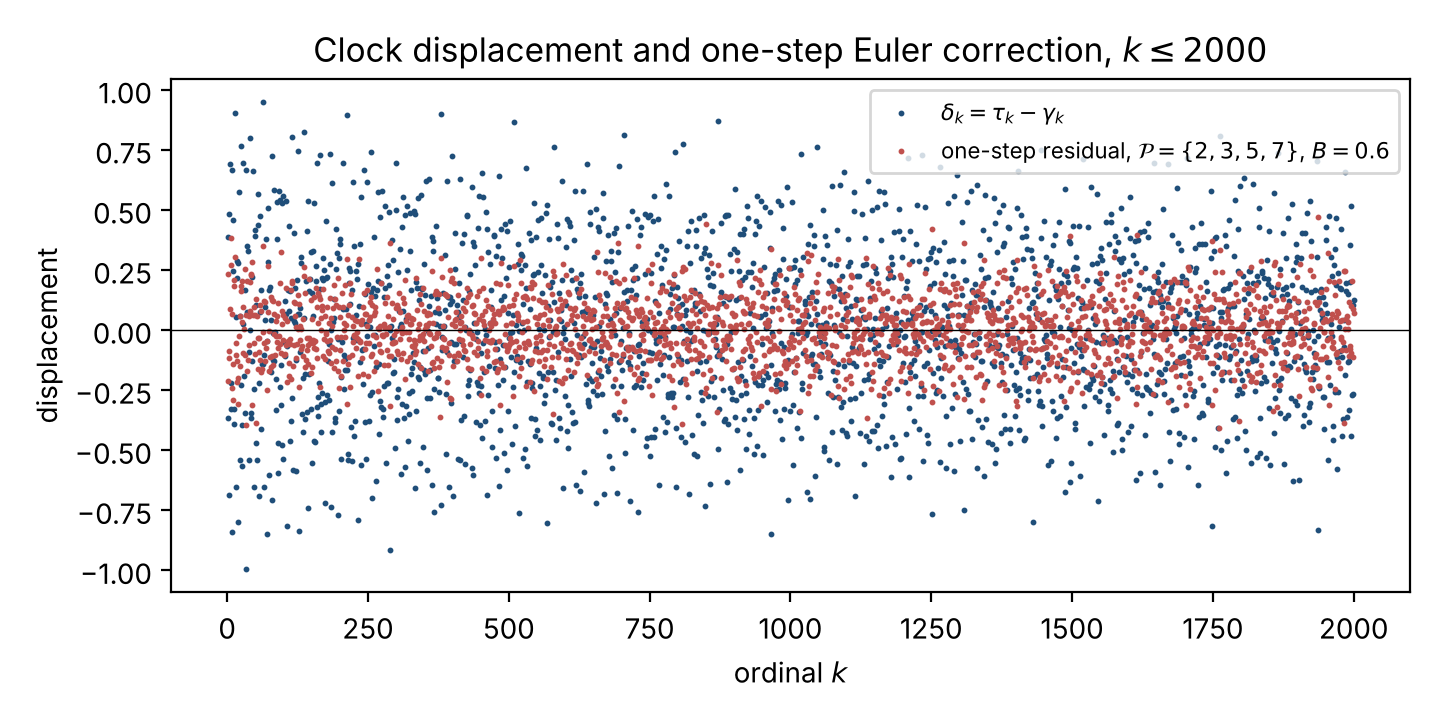
\includegraphics[width=0.92\textwidth]{fig01_displacement_first2000.png}
\caption{The displacement $\delta_k=\tau_k-\gamma_k$ and the residual of the one-step clock with $P=\{2,3,5,7\}$ and $B=0.6$, for $k\le2000$.}
\label{fig:displacement}
\end{figure}

\begin{figure}[htbp]
\centering
\includegraphics[width=0.92\textwidth]{fig02_rms_by_height.png}
\caption{RMS of the residual in logarithmic bins of $k$ for the five methods of Table~\CGref{tab:methods}.}
\label{fig:rms_height}
\end{figure}

\begin{figure}[htbp]
\centering
\includegraphics[width=0.92\textwidth]{fig08_max_by_window.png}
\caption{Maximum of $|$residual$|$ in each window for the five methods of Table~\CGref{tab:methods}; the dotted line is $\frac12$.}
\label{fig:max_window}
\end{figure}

\subsection{The optimal cutoff grows with the height}
\label{subsec:optimal_cutoff}

\begin{experiment}\label{exp:optimal_cutoff}
Object: RMS of $\delta_k^{X}$ (no saturation) as a function of the cutoff $X$, for $40$ cutoffs between $2$ and $1999$, and the minimizing cutoff in each window. Range: the six windows. Expected outcome: the ordinal-defect theorem motivates testing cutoffs that grow with height, but does not predict the optimum of this one-step residual. Observed outcome: Table~\CGref{tab:optimal_cutoff}, Figures~\CGref{fig:rms_cutoff} and \CGref{fig:optimal_cutoff}, and the full scan in Tables~\CGref{tab:scan_rms}--\CGref{tab:scan_max}. The optimal cutoff increases from $7$ to $907$; the least-squares fit $\log X_{\rm opt}=\theta\log(\tau/2\pi)$ over windows $2$--$6$ gives $\theta=0.5744$. Near the optimum the RMS curves are flat: in the top window the RMS is $0.064467$ at $X=701$, $0.064271$ at $X=907$ and $0.064283$ at $X=1009$. The fit is exploratory: these five windows were also used to assess it, and no independent validation window is claimed. The flatness near the minimum limits the precision with which an exponent can be inferred.
\end{experiment}

\begin{table}[htbp]
\centering
\small
\begin{tabular}{lrrrr}
\toprule
window & $X_{\rm opt}$ & RMS at $X_{\rm opt}$ & median $\log(\tau_k/2\pi)$ & RMS of $\delta_k$\\
\midrule
$(0,10^3]$ & 7 & 0.163507 & 4.8617 & 0.358739\\
$(10^3,10^4]$ & 43 & 0.089165 & 6.8465 & 0.274177\\
$(10^4,10^5]$ & 151 & 0.076935 & 8.8540 & 0.226352\\
$(10^5,5\cdot10^5]$ & 401 & 0.069779 & 10.3736 & 0.199294\\
$(5\cdot10^5,10^6]$ & 701 & 0.066360 & 11.2050 & 0.186722\\
$(10^6,K]$ & 907 & 0.064271 & 11.8382 & 0.178900\\
\bottomrule
\end{tabular}
\caption{RMS-optimal prime cutoff of the one-step clock (no saturation) in each window (Experiment~\CGref{exp:optimal_cutoff}).}
\label{tab:optimal_cutoff}
\end{table}

\begin{figure}[htbp]
\centering
\includegraphics[width=0.92\textwidth]{fig03_rms_vs_cutoff.png}
\caption{RMS of the one-step residual against the cutoff $X$ (primes $p\le X$, full local factors), by window; dots mark the minimum of each window.}
\label{fig:rms_cutoff}
\end{figure}

\begin{figure}[htbp]
\centering
\includegraphics[width=0.7\textwidth]{fig04_optimal_cutoff.png}
\caption{Logarithm of the optimal cutoff against the median of $\log(\tau_k/2\pi)$ in each window, with the least-squares line through the origin fitted on windows $2$--$6$.}
\label{fig:optimal_cutoff}
\end{figure}

\begin{experiment}\label{exp:saturation}
Object: global maximum of $|\delta_k^{X,B}|$, its location, the number of residuals $\ge\frac12$, the RMS, and the residual at $k=258318$, for the fixed cutoffs $11\le X\le71$ and $B\in\{0.5,0.6,0.7\}$. Range: $1\le k\le K$. Expected outcome: none from the theory, which says nothing about finite maxima (Proposition~\CGref{prop:fixed_sup} concerns the limit). Observed outcome: Table~\CGref{tab:saturation}. For $B=0.5$ and $X\ge13$ the maximum $0.493711$ at $k=34$ comes from the saturation itself: the bare residual there is $0.993711$. With $B=0.6$, the cutoffs $X\in\{13,17,31\}$ and all $37\le X\le71$ give a maximum below $\frac12$ over the $2\,001\,052$ zeros, the smallest being $0.457259$ for $X=61$.
\end{experiment}

\subsection{Mean-square gain and projections}
\label{subsec:gain_projection}

\begin{experiment}\label{exp:gain}
Object: the gain $\langle s_k^2\rangle-\langle(s_k-S_P(\tau_k))^2\rangle$ for $P=\{2,3,5,7\}$ and $P=\{p\le61\}$ with full local factors, compared with $c_P$ of \CGeqref{eq:cP_def}. Range: the six windows. Expected outcome: by Corollary~\CGref{cor:gain} and Remark~\CGref{rem:gain_full_factors} (conditional on Hypothesis~\CGref{hyp:L}), the gain of each finite truncation tends to its $v_A$, and $v_A\uparrow c_P$. Observed outcome: Table~\CGref{tab:gain} and Figure~\CGref{fig:gain}. The gain increases with the height towards $c_P$, from $0.056957$ to $0.064441$ for $c_P=0.066252$, and from $0.047822$ to $0.087434$ for $c_P=0.093853$. The mean square $\langle s_k^2\rangle$ increases from $0.067170$ to $0.113224$, as Theorem~\CGref{thm:clock_moments} predicts qualitatively; the theorem determines only the leading term $(2\pi^2)^{-1}\log\log T$ and not the constant.
\end{experiment}

\begin{table}[htbp]
\centering
\small
\begin{tabular}{lrrrrr}
\toprule
window & $\langle s_k^2\rangle$ & gain, $P_7$ & $c_{P_7}$ & gain, $P_{61}$ & $c_{P_{61}}$\\
\midrule
$(0,10^3]$ & 0.067170 & 0.056957 & 0.066252 & 0.047822 & 0.093853\\
$(10^3,10^4]$ & 0.085195 & 0.063224 & 0.066252 & 0.075868 & 0.093853\\
$(10^4,10^5]$ & 0.098097 & 0.063878 & 0.066252 & 0.084636 & 0.093853\\
$(10^5,5\cdot10^5]$ & 0.106325 & 0.064185 & 0.066252 & 0.086367 & 0.093853\\
$(5\cdot10^5,10^6]$ & 0.110476 & 0.064339 & 0.066252 & 0.087027 & 0.093853\\
$(10^6,K]$ & 0.113224 & 0.064441 & 0.066252 & 0.087434 & 0.093853\\
\bottomrule
\end{tabular}
\caption{Mean-square gain of a fixed Euler phase against its limit $c_P$; $P_7=\{2,3,5,7\}$, $P_{61}=\{p\le61\}$ (Experiment~\CGref{exp:gain}).}
\label{tab:gain}
\end{table}

\begin{figure}[htbp]
\centering
\includegraphics[width=0.92\textwidth]{fig07_gain_vs_theory.png}
\caption{Measured mean-square gain of a fixed Euler phase in each window (markers) and the constants $c_P$ (dashed).}
\label{fig:gain}
\end{figure}

\begin{experiment}\label{exp:projection}
Object: the normalized projections $\rho_n=-2\pi\sqrt n\,\langle s_k\sin(\tau_k\log n)\rangle$ for $2\le n\le64$. Range: $10^6<k\le K$, where the median of $\log(\tau_k/2\pi)$ is $11.8382$. Expected outcome: $\rho_n\to\Lambda(n)/\log n$ by Theorem~\CGref{thm:projection} (conditional on Hypothesis~\CGref{hyp:L}), with the second-order correction \CGeqref{eq:second_order} at finite height (Heuristic~\CGref{heur:second_order}). Observed outcome: Table~\CGref{tab:projection} and Figure~\CGref{fig:projection}. For primes $\rho_p$ lies between $0.864$ and $0.979$; for prime squares between $0.526$ and $0.576$; over $n=p^aq^b\le64$ the largest deviation from \CGeqref{eq:second_order} is $0.0632$; the largest $|\rho_n|$ over integers which are not prime powers is $0.2936$, and the largest deviation from $\Lambda(n)/\log n$ over prime powers is $0.1356$.
\end{experiment}

\begin{figure}[htbp]
\centering
\includegraphics[width=0.92\textwidth]{fig05_projection_coefficients.png}
\caption{Normalized projections $\rho_n$ of the displacement on $\sin(\tau_k\log n)$, $10^6<k\le K$, with the first-order limit $\Lambda(n)/\log n$ and the second-order prediction \CGeqref{eq:second_order}.}
\label{fig:projection}
\end{figure}

\subsection{The extreme residual: a close pair of zeros}
\label{subsec:close_pair}

\begin{experiment}\label{exp:close_pair}
Object: the zero at which the fixed set $P=\{2,3,5,7\}$ with $B=0.6$ attains its largest residual. Range: $258315\le k\le258321$. Expected outcome: a large $|s_k|$, which by \CGeqref{eq:sawtooth_sandwich} forces a large value of $|S|$ nearby. Observed outcome: Table~\CGref{tab:close_pair} and Figure~\CGref{fig:close_pair}. The ordinates $\gamma_{258317}=175681.649131916$ and $\gamma_{258318}=175681.715894456$ form a close pair with normalized gap $0.1088$ (rank $2371$ among $2\,001\,051$ gaps), followed by a normalized gap $2.6587$. The midpoint value is $S(\gamma_{258318})=1.0394$ and $\delta_{258318}=0.6379$. The residuals at $k=258318$ are $0.5223$ ($P=\{2,3,5,7\}$, $B=0.6$), $0.2345$ ($P=\{p\le61\}$, $B=0.6$), $0.3373$ ($P=\{p\le1999\}$) and $0.2031$ (ordinal-dependent cutoff).
\end{experiment}

\begin{table}[htbp]
\centering
\small
\begin{tabular}{rrrrrr}
\toprule
$k$ & $\gamma_k$ & $\tau_k$ & $\delta_k$ & $\gamma_{k+1}-\gamma_k$ & normalized gap\\
\midrule
258315 & 175680.155201189 & 175680.512721900 & $+0.3575$ & 0.8010 & 1.3053\\
258316 & 175680.956210354 & 175681.126401291 & $+0.1702$ & 0.6929 & 1.1291\\
258317 & 175681.649131916 & 175681.740080472 & $+0.0909$ & 0.0668 & 0.1088\\
258318 & 175681.715894456 & 175682.353759444 & $+0.6379$ & 1.6316 & 2.6587\\
258319 & 175683.347455659 & 175682.967438207 & $-0.3800$ & 0.5181 & 0.8443\\
258320 & 175683.865589247 & 175683.581116760 & $-0.2845$ & 0.4856 & 0.7914\\
258321 & 175684.351235152 & 175684.194795104 & $-0.1564$ & 0.3002 & 0.4892\\
\bottomrule
\end{tabular}
\caption{Ordinates, clock and gaps around the close pair $k=258317,258318$; the normalized gap is $(\gamma_{k+1}-\gamma_k)\log(\gamma_k/2\pi)/2\pi$ (Experiment~\CGref{exp:close_pair}).}
\label{tab:close_pair}
\end{table}

\begin{figure}[htbp]
\centering
\includegraphics[width=0.92\textwidth]{fig06_close_pair.png}
\caption{Zeros, clock and one-step clocks around the close pair $k=258317,258318$.}
\label{fig:close_pair}
\end{figure}

\subsection{Direct defects and moving-prime responses}
\label{subsec:direct_extensions}
\begin{experiment}[Direct measurement of the theorem's observable]\label{exp:direct_defects}
For $T=2^r$, $r\in\{14,16,18,19\}$, and $c\in\{1/10,1/5,1/3,1/2\}$, we compute the full local-factor phase at the true ordinates, with one cutoff $X=T^c$ throughout each window, and form $u_k(X)=k-1/2-\NO(\gamma_k)-S_X(\gamma_k)$. The numbers of ordinates are respectively $21\,519$, $100\,536$, $459\,982$ and $977\,804$. The last window, entirely contained in the data, gives Table~\CGref{tab:direct_top}; all sixteen measurements and the one-step comparison appear in Appendix~\CGref{sec:extension_calculations}. Exponents smaller than $1/10$ on the stated trial grid give $X<2$ at these heights and are excluded, consistently with the theorem's range. The finite means do not identify a limiting constant at fixed $c$.
\end{experiment}
\begin{table}[htbp]
\centering\small
\begin{tabular}{rrrrr}
\toprule
$c$ & $\#\{p\le X\}$ & $\langle u_k(X)^2\rangle$ & $\frac1{2\pi^2}\log(1/c)$ & $\langle r_k(X)^2\rangle$\\
\midrule
$1/10$ & 2 & 0.065599 & 0.116650 & 0.065517\\
$1/5$ & 6 & 0.040530 & 0.081535 & 0.040623\\
$1/3$ & 22 & 0.022911 & 0.055656 & 0.023446\\
$1/2$ & 128 & 0.012187 & 0.035115 & 0.014567\\
\bottomrule
\end{tabular}
\caption{Direct ordinal defects on $2^{19}<\gamma_k\le2^{20}$, with $977\,804$ ordinates and $X=(2^{19})^c$. The one-step residual has no saturation. These are different observables.}
\label{tab:direct_top}
\end{table}

\begin{experiment}[Individual-prime and grouped responses]\label{exp:moving_responses}
For every one of the $2262$ primes $p\le20000$ we compute both responses in \CGeqref{eq:two_responses} on the five ordinal windows after $k=1000$. We use the exact $s_k=k-1/2-\NO(\gamma_k)$, and assign to a prime the horizontal coordinate $\theta=\log p/\operatorname{median}_{k\in I}\log(\tau_k/2\pi)$. These are finite ordinal windows, rather than the dyadic height windows of the arithmetic hypotheses. Only primes with $0<\theta<1$ are compared with $R(\theta)$. The complete individual responses are retained in the companion CSV, and Table~\CGref{tab:response_errors} distinguishes individual errors from averages in bins of width $0.05$, using only bins with at least five primes. The grouped comparison supports the shape of the candidate; it supplies neither a uniform individual-prime error of $0.03$ nor an asymptotic proof.
\end{experiment}
\begin{table}[htbp]
\centering\small
\begin{tabular}{lrrrr}
\toprule
ordinal window & primes with $\theta<1$ & max individual error & RMS error & max bin-mean error\\
\midrule
$(10^3,10^4]$ & 159 & 0.34557 & 0.09425 & 0.02637\\
$(10^4,10^5]$ & 901 & 0.44085 & 0.08511 & 0.02371\\
$(10^5,5\cdot10^5]$ & 2262 & 0.27857 & 0.06429 & 0.02972\\
$(5\cdot10^5,10^6]$ & 2262 & 0.31682 & 0.06086 & 0.03531\\
$(10^6,K]$ & 2262 & 0.16425 & 0.03309 & 0.01951\\
\bottomrule
\end{tabular}
\caption{Errors of $\rho_p^\gamma-R(\theta)$ in Experiment~\CGref{exp:moving_responses}. Bin errors are absolute means of the signed individual errors, not maxima over individual primes.}
\label{tab:response_errors}
\end{table}
In the top window, the means of $\rho_p^\tau$ in the bins $[0.65,0.70)$, $[0.70,0.75)$ and $[0.75,0.80)$ are $0.66402$, $0.65240$ and $0.66417$. This finite-height plateau is different from $R(\theta)$ and does not establish a universal same-clock law. In particular, the prime near $p=17333$ has an individual $\rho_p^\gamma$ error about $0.16425$, despite the much smaller bin-mean discrepancies.

\section{Discussion and conclusions}
\label{sec:discussion}
\subsection{Status and significance of the results}
\label{subsec:status}
The exact jump identity, the moment and cutoff theorems, the finite-window gain, matrix projection and Fourier reduction are unconditional. They use the genuine zeros $\rho_k=\beta_k+i\gamma_k$ with no restriction on $\beta_k$ and allow repeated ordinates. Their analytic ingredients are the classical results collected in Section~\CGref{sec:known_results}. The zero-displacement limit superior is a consequence of Bellotti--Wong after inversion, and the moment asymptotics follow from Selberg through the exact identity. These deductions are distinguished from the classical input itself.

Theorem~\CGref{thm:projection} and Corollary~\CGref{cor:gain} assume the fixed-frequency Landau hypothesis, which RH implies. Theorem~\CGref{thm:sine_kernel} and Proposition~\CGref{prop:kernel_integral} are exact results for the stated determinantal model. The identification $\rho^\gamma(\theta)=1-\Phi(\theta)$ for zeta requires the additional uniform one-particle input and weighted arithmetic bridge. The second-order composite-frequency formula of Heuristic~\CGref{heur:second_order} remains a heuristic. All scanned optima, finite maxima and empirical response curves are numerical observations.

\subsection{What is proved about prime correction}
\label{subsec:what_proved}
Theorem~\CGref{thm:main} answers an arithmetic question about the truncated equation at true ordinates: fixed primes leave a divergent mean-square ordinal defect, whereas $X=T^c$, $0<c\le1/2$, keeps it bounded, and boundedness in this range requires $\log X\asymp\log T$. It does not determine the constant at fixed $c$, select a root when the model is not monotone, or prove that a fixed positive exponent is optimal for the one-step clock.

For the computable clock correction, \CGeqref{eq:full_factor_gain} and Proposition~\CGref{prop:matrix_projection} identify exactly which finite-window information is needed: same-clock responses, prime-power contributions and the Gram matrix. These formulas remain valid at finite height without replacing cross terms by independence. A theorem for a universal $\rho^\tau$ and uniform estimates for growing Gram matrices would convert this accounting into an asymptotic predictor. A pointwise error bound additionally requires an individual bound for the reconstruction residual.

\subsection{The contribution of the prime-resonant calculation}
\label{subsec:novelty}
The proposed contribution is the connection between the ordinal defect, an exact shifted correlation of the zero measure, and a determinantal response that evaluates to the same parameter-free function $\Phi(\theta)$. The general cumulant formalism and spectral-projection overlap calculation are standard tools; they are not claimed as new. The specific quadrature identity for the defect, its uniform cutoff dichotomy, the exact finite-window accounting and the prime-resonant interpretation are the results and formulations established here. Priority for these specific combinations has not been settled by an exhaustive literature comparison.

The support calculation has a concrete consequence: the model response is zero throughout the restricted-support region \CGeqref{eq:kernel_support_barrier}, while the weighted integral giving $\Phi$ comes entirely from outside it. This identifies the missing arithmetic information rather than concealing it in a general appeal to GUE. The significance is an exact, testable target at scale $p^{-1/2}$, together with a rigorous distinction between what the model proves and what remains to be shown for zeta.

\begin{remark}\label{rem:no_spacing}
The cutoff and displacement moment theorems do not imply local random-matrix spacing statistics. Changing each ordinate by at most $\epsilon/\lL(\gamma_k)$ changes its ordinal displacement by at most $\epsilon(1+o(1))$, so the leading moment growth can coexist with different local spacing statistics. The determinantal calculation is a separate model with its own hypotheses.
\end{remark}

\section{Open problems and further computations}
\label{sec:open_questions}
\begin{question}\label{q:constant}
For fixed $c\in(0,1/2]$, does the bounded sequence of means of $u_k(T^c)^2$ have a limit of the form $(2\pi^2)^{-1}\log(1/c)+\kappa(c)$? The present error is $O_c(1)$ and does not prove existence of this limit or independence of $\kappa(c)$ from $c$. Determining it requires evaluation of mixed Selberg remainders and prime-power terms, not only upper bounds.
\end{question}
\begin{question}\label{q:large_c}
Can the cutoff theorem be extended past $c=1/2$? Its fourth-moment proof uses $X^2\le T$; longer prime polynomials require further moment or correlation estimates. No extension to $c\le2$ is asserted.
\end{question}
\begin{question}\label{q:per_ordinate}
Does the same estimate hold for the genuinely varying cutoff $X_k=(\tau_k/2\pi)^\theta$? A rule constant on each dyadic window is already covered. Passing to a cutoff varying at every ordinate requires an additional maximal estimate or another uniform argument; a bounded ratio of the two cutoffs is not a proof.
\end{question}
\begin{question}\label{q:one_step}
Can one establish a universal same-clock law $\rho^\tau(\theta)$, with uniform control of the Gram matrix and prime-power terms sufficient to optimize the exact gain? No asymptotic formula for the optimal one-step exponent or its residual variance is assumed.
\end{question}
\begin{question}\label{q:prime_bridge}
Can the real or complex weighted arithmetic bridge \CGeqref{eq:weighted_arithmetic_bridge} be proved for moving primes? A proof must control the full weighted integral, including tails, and distinguish the real-part statement from its stronger complex version.
\end{question}
\subsection{Computational follow-up}
\label{q:experiment_uk}
The direct-defect measurements below contrast the quantity in Theorem~\CGref{thm:main}. Further computations can solve $F_X(t)=k-1/2$ under the monotonicity condition of Proposition~\CGref{prop:localization}, and then record the solution, the minimum derivative and the residual of the equation. Training response coefficients on one window and evaluating them on a later window is required for an independent predictive test. No observed finite maximum is extrapolated to a uniform theorem.
\subsection{Dirichlet functions}
\label{q:generalization}
The exact identity of Theorem~\CGref{thm:identity_general} applies to any counting staircase and $C^1$ model, so it also applies to a consistently normalized Dirichlet zero count. An analytic cutoff theorem for a primitive Dirichlet character would additionally require the corresponding Selberg approximation, the conductor and parity normalization, and uniformity in the conductor if it varies; it is not proved here. Related individual-zero equations and prime approximations appear in \cite{FrancaLeClair2015,Fujii1974}.

\clearpage
\begin{thebibliography}{99}

\bibitem{BellottiWong2025}
C.~Bellotti and P.-J. Wong, Improved estimates for the argument and zero-counting function of the Riemann zeta-function, \emph{Math. Comp.} (2025, published online), \href{https://doi.org/10.1090/mcom/4133}{doi:10.1090/mcom/4133}; arXiv:2412.15470.

\bibitem{Billingsley1995}
P.~Billingsley, \emph{Probability and Measure}, 3rd ed., Wiley, New York, 1995. (No DOI.)

\bibitem{Corless1996}
R.~M. Corless, G.~H. Gonnet, D.~E.~G. Hare, D.~J. Jeffrey and D.~E. Knuth, On the Lambert $W$ function, \emph{Adv. Comput. Math.} \textbf{5} (1996), 329--359, \href{https://doi.org/10.1007/BF02124750}{doi:10.1007/BF02124750}.

\bibitem{FrancaLeClair2014}
G.~Fran\c{c}a and A.~LeClair, Statistical and other properties of Riemann zeros based on an explicit equation for the $n$-th zero on the critical line, preprint, arXiv:1307.8395 (2013), \href{https://doi.org/10.48550/arXiv.1307.8395}{doi:10.48550/arXiv.1307.8395}.

\bibitem{FrancaLeClair2015}
G.~Fran\c{c}a and A.~LeClair, Transcendental equations satisfied by the individual zeros of Riemann $\zeta$, Dirichlet and modular $L$-functions, \emph{Commun. Number Theory Phys.} \textbf{9} (2015), no.~1, 1--50, \href{https://doi.org/10.4310/CNTP.2015.v9.n1.a1}{doi:10.4310/CNTP.2015.v9.n1.a1}; arXiv:1502.06003.

\bibitem{Fujii1974}
A.~Fujii, On the zeros of Dirichlet $L$-functions. I, \emph{Trans. Amer. Math. Soc.} \textbf{196} (1974), 225--235, \href{https://doi.org/10.1090/S0002-9947-1974-0349603-2}{doi:10.1090/S0002-9947-1974-0349603-2}.

\bibitem{Gonek1993}
S.~M. Gonek, An explicit formula of Landau and its applications to the theory of the zeta-function, in: \emph{A Tribute to Emil Grosswald: Number Theory and Related Analysis}, Contemp. Math. \textbf{143}, Amer. Math. Soc., Providence, RI, 1993, 395--413, \href{https://doi.org/10.1090/conm/143/1210528}{doi:10.1090/conm/143/1210528}.

\bibitem{Gonek2012}
S.~M. Gonek, Finite Euler products and the Riemann hypothesis, \emph{Trans. Amer. Math. Soc.} \textbf{364} (2012), 2157--2191, \href{https://doi.org/10.1090/S0002-9947-2011-05546-7}{doi:10.1090/S0002-9947-2011-05546-7}; arXiv:0704.3448.

\bibitem{GrahamKolesnik1991}
S.~W. Graham and G.~Kolesnik, \emph{Van der Corput's Method of Exponential Sums}, London Math. Soc. Lecture Note Ser. \textbf{126}, Cambridge University Press, Cambridge, 1991, \href{https://doi.org/10.1017/CBO9780511661976}{doi:10.1017/CBO9780511661976}.

\bibitem{HasanalizadeShenWong2022}
E.~Hasanalizade, Q.~Shen and P.-J. Wong, Counting zeros of the Riemann zeta function, \emph{J. Number Theory} \textbf{235} (2022), 219--241, \href{https://doi.org/10.1016/j.jnt.2021.06.032}{doi:10.1016/j.jnt.2021.06.032}; arXiv:2107.06506.

\bibitem{Korolev2012}
M.~A. Korolev, On Gram's law in the theory of the Riemann zeta function, \emph{Izv. Math.} \textbf{76} (2012), no.~2, 275--309, \href{https://doi.org/10.1070/IM2012v076n02ABEH002583}{doi:10.1070/IM2012v076n02ABEH002583}; Russian original \emph{Izv. Ross. Akad. Nauk Ser. Mat.} \textbf{76} (2012), no.~2, 67--102, \href{https://doi.org/10.4213/im5558}{doi:10.4213/im5558}; arXiv:1011.3997.

\bibitem{Landau1912}
E.~Landau, \"Uber die Nullstellen der Zetafunktion, \emph{Math. Ann.} \textbf{71} (1912), 548--564, \href{https://doi.org/10.1007/BF01456808}{doi:10.1007/BF01456808}.

\bibitem{LeClair2021}
A.~LeClair, Riemann hypothesis and random walks: the zeta case, \emph{Symmetry} \textbf{13} (2021), no.~11, 2014, \href{https://doi.org/10.3390/sym13112014}{doi:10.3390/sym13112014}; arXiv:1601.00914.

\bibitem{Littlewood1924}
J.~E. Littlewood, On the zeros of the Riemann zeta-function, \emph{Proc. Cambridge Philos. Soc.} \textbf{22} (1924), 295--318, \href{https://doi.org/10.1017/S0305004100014225}{doi:10.1017/S0305004100014225}.

\bibitem{Mertens1874}
F.~Mertens, Ein Beitrag zur analytischen Zahlentheorie, \emph{J. Reine Angew. Math.} \textbf{78} (1874), 46--62, \href{https://doi.org/10.1515/crll.1874.78.46}{doi:10.1515/crll.1874.78.46}.

\bibitem{MontgomeryVaughan1974}
H.~L. Montgomery and R.~C. Vaughan, Hilbert's inequality, \emph{J. London Math. Soc. (2)} \textbf{8} (1974), 73--82, \href{https://doi.org/10.1112/jlms/s2-8.1.73}{doi:10.1112/jlms/s2-8.1.73}.

\bibitem{Selberg1946a}
A.~Selberg, Contributions to the theory of the Riemann zeta-function, \emph{Arch. Math. Naturvid.} \textbf{48} (1946), no.~5, 89--155. (No DOI.)

\bibitem{Selberg1946b}
A.~Selberg, Contributions to the theory of Dirichlet's $L$-functions, \emph{Skr. Norske Vid.-Akad. Oslo I} \textbf{1946}, no.~3, 2--62. (No DOI.)

\bibitem{Titchmarsh1986}
E.~C. Titchmarsh, \emph{The Theory of the Riemann Zeta-Function}, 2nd ed., revised by D.~R. Heath-Brown, Clarendon Press, Oxford, 1986. (No DOI.)

\bibitem{Trudgian2014}
T.~S. Trudgian, An improved upper bound for the argument of the Riemann zeta-function on the critical line II, \emph{J. Number Theory} \textbf{134} (2014), 280--292, \href{https://doi.org/10.1016/j.jnt.2013.07.017}{doi:10.1016/j.jnt.2013.07.017}; arXiv:1208.5846.

\end{thebibliography}
\clearpage

\appendix

\section{Complete tables}
\label{sec:appendix_tables}

\begin{center}
\small
\begin{longtable}{rrrrrrr}
\caption{RMS of $\delta_k^X$ (no saturation) for all cutoffs of the scan of Experiment~\CGref{exp:optimal_cutoff}.}\label{tab:scan_rms}\\
\toprule
$X$ & $(0,10^3]$ & $(10^3,10^4]$ & $(10^4,10^5]$ & $(10^5,5\cdot10^5]$ & $(5\cdot10^5,10^6]$ & $(10^6,K]$\\
\midrule
\endfirsthead
\toprule
$X$ & $(0,10^3]$ & $(10^3,10^4]$ & $(10^4,10^5]$ & $(10^5,5\cdot10^5]$ & $(5\cdot10^5,10^6]$ & $(10^6,K]$\\
\midrule
\endhead
2 & 0.264585 & 0.221853 & 0.189628 & 0.169743 & 0.160181 & 0.154125\\
3 & 0.200546 & 0.182692 & 0.162903 & 0.148543 & 0.141254 & 0.136519\\
5 & 0.175536 & 0.157325 & 0.145975 & 0.135250 & 0.129435 & 0.125551\\
7 & 0.163507 & 0.138018 & 0.133227 & 0.125335 & 0.120648 & 0.117413\\
11 & 0.167491 & 0.125933 & 0.125019 & 0.118978 & 0.115014 & 0.112199\\
13 & 0.180112 & 0.115143 & 0.117861 & 0.113445 & 0.110121 & 0.107676\\
17 & 0.189732 & 0.107018 & 0.112357 & 0.109187 & 0.106362 & 0.104196\\
19 & 0.203848 & 0.099967 & 0.107341 & 0.105291 & 0.102932 & 0.101027\\
23 & 0.207822 & 0.094970 & 0.103192 & 0.102058 & 0.100080 & 0.098398\\
29 & 0.220519 & 0.091980 & 0.099933 & 0.099516 & 0.097835 & 0.096324\\
31 & 0.230788 & 0.089845 & 0.096818 & 0.097113 & 0.095707 & 0.094360\\
37 & 0.233278 & 0.089201 & 0.094209 & 0.095126 & 0.093936 & 0.092724\\
43 & 0.247108 & 0.089165 & 0.089653 & 0.091595 & 0.090813 & 0.089816\\
53 & 0.253280 & 0.090105 & 0.085984 & 0.088604 & 0.088177 & 0.087369\\
61 & 0.261896 & 0.091200 & 0.083253 & 0.086131 & 0.085995 & 0.085356\\
71 & 0.272840 & 0.092404 & 0.081157 & 0.083975 & 0.084099 & 0.083607\\
83 & 0.279043 & 0.094679 & 0.078846 & 0.081114 & 0.081573 & 0.081281\\
97 & 0.279760 & 0.096097 & 0.077984 & 0.079519 & 0.080174 & 0.079986\\
113 & 0.305237 & 0.099735 & 0.077086 & 0.076058 & 0.077117 & 0.077155\\
131 & 0.303814 & 0.101313 & 0.076968 & 0.075024 & 0.076116 & 0.076235\\
151 & 0.309424 & 0.104066 & 0.076935 & 0.073336 & 0.074335 & 0.074579\\
173 & 0.323001 & 0.106809 & 0.077044 & 0.072094 & 0.072794 & 0.073149\\
199 & 0.322057 & 0.110538 & 0.077336 & 0.070915 & 0.070796 & 0.071304\\
229 & 0.322766 & 0.112658 & 0.077638 & 0.070557 & 0.069704 & 0.070261\\
263 & 0.335293 & 0.115531 & 0.078195 & 0.070231 & 0.068448 & 0.068864\\
307 & 0.339800 & 0.119016 & 0.078840 & 0.069985 & 0.067633 & 0.067458\\
353 & 0.342957 & 0.122519 & 0.079635 & 0.069831 & 0.067253 & 0.066262\\
401 & 0.358302 & 0.125367 & 0.080542 & 0.069779 & 0.066961 & 0.065561\\
461 & 0.359151 & 0.128498 & 0.081570 & 0.069855 & 0.066669 & 0.065176\\
523 & 0.354759 & 0.131831 & 0.082601 & 0.069960 & 0.066526 & 0.064877\\
601 & 0.367055 & 0.134709 & 0.083735 & 0.070147 & 0.066431 & 0.064663\\
701 & 0.376638 & 0.138525 & 0.085322 & 0.070484 & 0.066360 & 0.064467\\
809 & 0.367728 & 0.141873 & 0.086526 & 0.070817 & 0.066390 & 0.064353\\
907 & 0.377272 & 0.144454 & 0.087902 & 0.071167 & 0.066521 & 0.064271\\
1009 & 0.387648 & 0.146798 & 0.089073 & 0.071525 & 0.066595 & 0.064283\\
1201 & 0.378526 & 0.151049 & 0.091182 & 0.072272 & 0.066845 & 0.064317\\
1409 & 0.381402 & 0.154503 & 0.092992 & 0.072896 & 0.067167 & 0.064412\\
1601 & 0.399367 & 0.158134 & 0.094832 & 0.073618 & 0.067469 & 0.064584\\
1801 & 0.389913 & 0.161587 & 0.096305 & 0.074283 & 0.067767 & 0.064768\\
1999 & 0.384555 & 0.163764 & 0.097502 & 0.074828 & 0.068088 & 0.064897\\
\bottomrule
\end{longtable}
\end{center}

\begin{center}
\small
\begin{longtable}{rrrrrrr}
\caption{Maximum of $|\delta_k^X|$ (no saturation) for all cutoffs of the scan of Experiment~\CGref{exp:optimal_cutoff}.}\label{tab:scan_max}\\
\toprule
$X$ & $(0,10^3]$ & $(10^3,10^4]$ & $(10^4,10^5]$ & $(10^5,5\cdot10^5]$ & $(5\cdot10^5,10^6]$ & $(10^6,K]$\\
\midrule
\endfirsthead
\toprule
$X$ & $(0,10^3]$ & $(10^3,10^4]$ & $(10^4,10^5]$ & $(10^5,5\cdot10^5]$ & $(5\cdot10^5,10^6]$ & $(10^6,K]$\\
\midrule
\endhead
2 & 0.714732 & 0.769491 & 0.692832 & 0.720658 & 0.661936 & 0.671779\\
3 & 0.778082 & 0.590169 & 0.597440 & 0.601584 & 0.561789 & 0.568719\\
5 & 1.374655 & 0.516964 & 0.542554 & 0.529087 & 0.499111 & 0.519284\\
7 & 1.363459 & 0.470967 & 0.477838 & 0.522347 & 0.484035 & 0.489293\\
11 & 1.508302 & 0.509751 & 0.476272 & 0.484013 & 0.461281 & 0.472383\\
13 & 1.890769 & 0.471351 & 0.485959 & 0.459791 & 0.471622 & 0.445972\\
17 & 2.030160 & 0.462473 & 0.484965 & 0.471862 & 0.452001 & 0.438833\\
19 & 2.579012 & 0.511457 & 0.473939 & 0.436459 & 0.420326 & 0.419404\\
23 & 2.086207 & 0.480575 & 0.516961 & 0.449248 & 0.426305 & 0.396139\\
29 & 2.532059 & 0.517976 & 0.486233 & 0.456782 & 0.425924 & 0.421632\\
31 & 2.731378 & 0.478395 & 0.503207 & 0.436347 & 0.394374 & 0.408531\\
37 & 2.436264 & 0.472277 & 0.467938 & 0.457662 & 0.402816 & 0.408334\\
43 & 2.920237 & 0.445443 & 0.482769 & 0.454351 & 0.425856 & 0.418435\\
53 & 2.844272 & 0.421161 & 0.474280 & 0.499673 & 0.435596 & 0.405677\\
61 & 2.717402 & 0.386775 & 0.457259 & 0.456272 & 0.432954 & 0.400144\\
71 & 3.238857 & 0.440040 & 0.447583 & 0.474087 & 0.436888 & 0.399374\\
83 & 2.963768 & 0.484372 & 0.467632 & 0.463983 & 0.438356 & 0.404333\\
97 & 2.894415 & 0.492464 & 0.483027 & 0.471593 & 0.460266 & 0.426854\\
113 & 3.849430 & 0.505889 & 0.513140 & 0.459718 & 0.483898 & 0.444630\\
131 & 3.439317 & 0.529451 & 0.517859 & 0.460881 & 0.484771 & 0.422286\\
151 & 3.367629 & 0.513247 & 0.525446 & 0.470577 & 0.482027 & 0.452456\\
173 & 3.996564 & 0.501890 & 0.549235 & 0.495148 & 0.456277 & 0.461665\\
199 & 3.365175 & 0.506558 & 0.523619 & 0.495310 & 0.458465 & 0.468141\\
229 & 3.335133 & 0.493618 & 0.528107 & 0.497048 & 0.468220 & 0.469958\\
263 & 4.072437 & 0.509804 & 0.557233 & 0.535397 & 0.479418 & 0.457026\\
307 & 3.875649 & 0.526799 & 0.546887 & 0.526425 & 0.467465 & 0.473187\\
353 & 3.465466 & 0.541694 & 0.561048 & 0.534833 & 0.473423 & 0.477070\\
401 & 4.309564 & 0.517594 & 0.555640 & 0.563591 & 0.504123 & 0.520443\\
461 & 4.028754 & 0.524278 & 0.544453 & 0.564897 & 0.521484 & 0.515423\\
523 & 3.255435 & 0.547997 & 0.577784 & 0.573315 & 0.492713 & 0.513253\\
601 & 4.111242 & 0.510670 & 0.585122 & 0.569968 & 0.507595 & 0.499887\\
701 & 4.359529 & 0.561843 & 0.576930 & 0.548586 & 0.495677 & 0.503530\\
809 & 3.399704 & 0.551479 & 0.599065 & 0.553709 & 0.486320 & 0.525568\\
907 & 4.022965 & 0.520528 & 0.588646 & 0.540603 & 0.524873 & 0.529711\\
1009 & 4.759390 & 0.506597 & 0.574853 & 0.553235 & 0.523729 & 0.521027\\
1201 & 3.414545 & 0.491973 & 0.602652 & 0.560114 & 0.551342 & 0.534354\\
1409 & 3.934751 & 0.472026 & 0.587566 & 0.572365 & 0.566273 & 0.533096\\
1601 & 4.812450 & 0.524598 & 0.593689 & 0.572861 & 0.554297 & 0.526446\\
1801 & 3.551103 & 0.528815 & 0.586851 & 0.576451 & 0.554530 & 0.526215\\
1999 & 3.247397 & 0.491263 & 0.618127 & 0.591452 & 0.552165 & 0.528267\\
\bottomrule
\end{longtable}
\end{center}

\begin{center}
\small
\begin{longtable}{rrrrrrr}
\caption{Fixed cutoffs and saturation levels over all $K$ zeros (Experiment~\CGref{exp:saturation}).}\label{tab:saturation}\\
\toprule
$X$ & $B$ & global max & $k$ at max & $\#\ge\frac12$ & RMS & residual at $k=258318$\\
\midrule
\endfirsthead
\toprule
$X$ & $B$ & global max & $k$ at max & $\#\ge\frac12$ & RMS & residual at $k=258318$\\
\midrule
\endhead
11 & 0.5 & 0.497093 & 1252 & 0 & 0.114954 & +0.468830\\
11 & 0.6 & 0.509751 & 1252 & 1 & 0.114954 & +0.468830\\
11 & 0.7 & 0.509751 & 1252 & 1 & 0.114954 & +0.468830\\
13 & 0.5 & 0.493711 & 34 & 0 & 0.109968 & +0.414562\\
13 & 0.6 & 0.485959 & 28074 & 0 & 0.109974 & +0.414562\\
13 & 0.7 & 0.485959 & 28074 & 0 & 0.109975 & +0.414562\\
17 & 0.5 & 0.493711 & 34 & 0 & 0.106136 & +0.377680\\
17 & 0.6 & 0.484965 & 28075 & 0 & 0.106150 & +0.377680\\
17 & 0.7 & 0.484965 & 28075 & 0 & 0.106153 & +0.377680\\
19 & 0.5 & 0.493711 & 34 & 0 & 0.102639 & +0.351715\\
19 & 0.6 & 0.511457 & 4988 & 1 & 0.102665 & +0.351715\\
19 & 0.7 & 0.511457 & 4988 & 1 & 0.102670 & +0.351715\\
23 & 0.5 & 0.493711 & 34 & 0 & 0.099739 & +0.321005\\
23 & 0.6 & 0.516961 & 28075 & 1 & 0.099777 & +0.321005\\
23 & 0.7 & 0.516961 & 28075 & 1 & 0.099784 & +0.321005\\
29 & 0.5 & 0.493711 & 34 & 0 & 0.097456 & +0.320746\\
29 & 0.6 & 0.517976 & 4988 & 1 & 0.097509 & +0.320746\\
29 & 0.7 & 0.517976 & 4988 & 1 & 0.097518 & +0.320746\\
31 & 0.5 & 0.493711 & 34 & 0 & 0.095297 & +0.286603\\
31 & 0.6 & 0.481293 & 28075 & 0 & 0.095364 & +0.286603\\
31 & 0.7 & 0.503207 & 31812 & 1 & 0.095375 & +0.286603\\
37 & 0.5 & 0.493711 & 34 & 0 & 0.093503 & +0.257718\\
37 & 0.6 & 0.472277 & 6709 & 0 & 0.093584 & +0.257718\\
37 & 0.7 & 0.481833 & 7 & 0 & 0.093598 & +0.257718\\
41 & 0.5 & 0.493711 & 34 & 0 & 0.091884 & +0.282516\\
41 & 0.6 & 0.480998 & 5444 & 0 & 0.091977 & +0.282516\\
41 & 0.7 & 0.481833 & 7 & 0 & 0.091994 & +0.282516\\
43 & 0.5 & 0.493711 & 34 & 0 & 0.090330 & +0.255696\\
43 & 0.6 & 0.482769 & 55259 & 0 & 0.090438 & +0.255696\\
43 & 0.7 & 0.482769 & 55259 & 0 & 0.090456 & +0.255696\\
47 & 0.5 & 0.493711 & 34 & 0 & 0.088909 & +0.233942\\
47 & 0.6 & 0.477323 & 30265 & 0 & 0.089031 & +0.233942\\
47 & 0.7 & 0.489035 & 31812 & 0 & 0.089052 & +0.233942\\
53 & 0.5 & 0.493711 & 34 & 0 & 0.087660 & +0.260451\\
53 & 0.6 & 0.474829 & 100674 & 0 & 0.087797 & +0.260451\\
53 & 0.7 & 0.499673 & 100674 & 0 & 0.087821 & +0.260451\\
59 & 0.5 & 0.493711 & 34 & 0 & 0.086551 & +0.239402\\
59 & 0.6 & 0.474829 & 100674 & 0 & 0.086700 & +0.239402\\
59 & 0.7 & 0.482408 & 100674 & 0 & 0.086726 & +0.239402\\
61 & 0.5 & 0.493711 & 34 & 0 & 0.085471 & +0.234496\\
61 & 0.6 & 0.457259 & 55259 & 0 & 0.085635 & +0.234496\\
61 & 0.7 & 0.481833 & 7 & 0 & 0.085663 & +0.234496\\
67 & 0.5 & 0.493711 & 34 & 0 & 0.084496 & +0.258256\\
67 & 0.6 & 0.474829 & 100674 & 0 & 0.084673 & +0.258256\\
67 & 0.7 & 0.481833 & 7 & 0 & 0.084704 & +0.258256\\
71 & 0.5 & 0.493711 & 34 & 0 & 0.083579 & +0.248477\\
71 & 0.6 & 0.458509 & 100674 & 0 & 0.083769 & +0.248477\\
71 & 0.7 & 0.481833 & 7 & 0 & 0.083803 & +0.248477\\
\bottomrule
\end{longtable}
\end{center}

\begin{center}
\small
\begin{longtable}{rrrrr}
\caption{Projections of the displacement, $10^6<k\le K$ (Experiment~\CGref{exp:projection}). Columns: $n$; $\langle\lL(\tau_k)\delta_k\sin(\tau_k\log n)\rangle$; $\rho_n$; $\Lambda(n)/\log n$; second-order prediction $\log n/(ab\log(\tau/2\pi))$ for $n=p^aq^b$ with the median of $\log(\tau_k/2\pi)$.}\label{tab:projection}\\
\toprule
$n$ & projection & $\rho_n$ & $\Lambda(n)/\log n$ & second order\\
\midrule
\endfirsthead
\toprule
$n$ & projection & $\rho_n$ & $\Lambda(n)/\log n$ & second order\\
\midrule
\endhead
2 & $-1.101798\cdot10^{-1}$ & 0.979032 & 1.000000 & --\\
3 & $-8.948284\cdot10^{-2}$ & 0.973824 & 1.000000 & --\\
4 & $-4.184672\cdot10^{-2}$ & 0.525861 & 0.500000 & --\\
5 & $-6.870881\cdot10^{-2}$ & 0.965333 & 1.000000 & --\\
6 & $-9.026866\cdot10^{-3}$ & 0.138929 & 0.000000 & 0.151353\\
7 & $-5.760368\cdot10^{-2}$ & 0.957589 & 1.000000 & --\\
8 & $-2.155326\cdot10^{-2}$ & 0.383035 & 0.333333 & --\\
9 & $-2.905212\cdot10^{-2}$ & 0.547620 & 0.500000 & --\\
10 & $-8.834723\cdot10^{-3}$ & 0.175539 & 0.000000 & 0.194504\\
11 & $-4.529915\cdot10^{-2}$ & 0.943987 & 1.000000 & --\\
12 & $-5.057500\cdot10^{-3}$ & 0.110079 & 0.000000 & 0.104952\\
13 & $-4.140890\cdot10^{-2}$ & 0.938092 & 1.000000 & --\\
14 & $-8.442033\cdot10^{-3}$ & 0.198468 & 0.000000 & 0.222926\\
15 & $-8.499428\cdot10^{-3}$ & 0.206831 & 0.000000 & 0.228754\\
16 & $-1.262904\cdot10^{-2}$ & 0.317402 & 0.250000 & --\\
17 & $-3.580933\cdot10^{-2}$ & 0.927685 & 1.000000 & --\\
18 & $-4.855880\cdot10^{-3}$ & 0.129445 & 0.000000 & 0.122078\\
19 & $-3.369338\cdot10^{-2}$ & 0.922787 & 1.000000 & --\\
20 & $-4.806896\cdot10^{-3}$ & 0.135070 & 0.000000 & 0.126528\\
21 & $-7.977501\cdot10^{-3}$ & 0.229698 & 0.000000 & 0.257177\\
22 & $-7.712575\cdot10^{-3}$ & 0.227295 & 0.000000 & 0.261106\\
23 & $-3.034556\cdot10^{-2}$ & 0.914406 & 1.000000 & --\\
24 & $-3.431327\cdot10^{-3}$ & 0.105620 & 0.000000 & 0.089486\\
25 & $-1.807767\cdot10^{-2}$ & 0.567927 & 0.500000 & --\\
26 & $-7.409792\cdot10^{-3}$ & 0.237396 & 0.000000 & 0.275218\\
27 & $-1.284469\cdot10^{-2}$ & 0.419359 & 0.333333 & --\\
28 & $-4.547679\cdot10^{-3}$ & 0.151199 & 0.000000 & 0.140739\\
29 & $-2.670938\cdot10^{-2}$ & 0.903738 & 1.000000 & --\\
30 & $-1.996010\cdot10^{-3}$ & 0.068692 & 0.000000 & --\\
31 & $-2.574513\cdot10^{-2}$ & 0.900649 & 1.000000 & --\\
32 & $-7.950979\cdot10^{-3}$ & 0.282602 & 0.200000 & --\\
33 & $-7.157940\cdot10^{-3}$ & 0.258360 & 0.000000 & 0.295357\\
34 & $-6.894815\cdot10^{-3}$ & 0.252605 & 0.000000 & 0.297879\\
35 & $-7.143158\cdot10^{-3}$ & 0.265524 & 0.000000 & 0.300327\\
36 & $-2.718760\cdot10^{-3}$ & 0.102495 & 0.000000 & 0.075677\\
37 & $-2.332464\cdot10^{-2}$ & 0.891447 & 1.000000 & --\\
38 & $-6.689950\cdot10^{-3}$ & 0.259116 & 0.000000 & 0.307274\\
39 & $-6.836467\cdot10^{-3}$ & 0.268253 & 0.000000 & 0.309468\\
40 & $-3.176432\cdot10^{-3}$ & 0.126226 & 0.000000 & 0.103869\\
41 & $-2.204080\cdot10^{-2}$ & 0.886746 & 1.000000 & --\\
42 & $-2.004407\cdot10^{-3}$ & 0.081619 & 0.000000 & --\\
43 & $-2.145466\cdot10^{-2}$ & 0.883966 & 1.000000 & --\\
44 & $-4.148809\cdot10^{-3}$ & 0.172914 & 0.000000 & 0.159829\\
45 & $-4.254161\cdot10^{-3}$ & 0.179308 & 0.000000 & 0.160778\\
46 & $-6.334462\cdot10^{-3}$ & 0.269941 & 0.000000 & 0.323413\\
47 & $-2.040786\cdot10^{-2}$ & 0.879076 & 1.000000 & --\\
48 & $-2.483491\cdot10^{-3}$ & 0.108109 & 0.000000 & 0.081752\\
49 & $-1.309455\cdot10^{-2}$ & 0.575928 & 0.500000 & --\\
50 & $-4.016163\cdot10^{-3}$ & 0.178433 & 0.000000 & 0.165228\\
51 & $-6.336008\cdot10^{-3}$ & 0.284303 & 0.000000 & 0.332129\\
52 & $-3.977664\cdot10^{-3}$ & 0.180223 & 0.000000 & 0.166885\\
53 & $-1.907514\cdot10^{-2}$ & 0.872540 & 1.000000 & --\\
54 & $-2.978449\cdot10^{-3}$ & 0.137520 & 0.000000 & 0.112319\\
55 & $-6.301149\cdot10^{-3}$ & 0.293617 & 0.000000 & 0.338507\\
56 & $-3.008650\cdot10^{-3}$ & 0.141464 & 0.000000 & 0.113343\\
57 & $-6.113419\cdot10^{-3}$ & 0.290002 & 0.000000 & 0.341525\\
58 & $-5.863989\cdot10^{-3}$ & 0.280600 & 0.000000 & 0.342994\\
59 & $-1.796165\cdot10^{-2}$ & 0.866866 & 1.000000 & --\\
60 & $-1.282342\cdot10^{-3}$ & 0.062411 & 0.000000 & --\\
61 & $-1.761495\cdot10^{-2}$ & 0.864423 & 1.000000 & --\\
62 & $-5.768611\cdot10^{-3}$ & 0.285395 & 0.000000 & 0.348627\\
63 & $-3.940823\cdot10^{-3}$ & 0.196534 & 0.000000 & 0.174989\\
64 & $-5.250276\cdot10^{-3}$ & 0.263908 & 0.166667 & --\\
\bottomrule
\end{longtable}
\end{center}

\section{Additional calculations and numerical parameters}
\label{sec:extension_calculations}
\subsection{Complete direct-defect calculation}
For each row we use all the ordinates in $(T,2T]$, the prime cutoff $X=T^c$, the principal argument of each Euler factor, and the exact ordinal defect. No fitting parameter or saturation is used. The last column is the ordinal residual of the one-step clock evaluated at $\tau_k$.
\begin{center}\small
\begin{longtable}{rrrrrr}
\caption{Complete direct-defect calculations.}\label{tab:direct_complete}\\
\toprule
$r$, $T=2^r$ & $c$ & $X$ & prime count & $\langle u_k^2\rangle$ & $\langle r_k^2\rangle$\\
\midrule\endfirsthead
\toprule
$r$ & $c$ & $X$ & prime count & $\langle u_k^2\rangle$ & $\langle r_k^2\rangle$\\
\midrule\endhead
14 & $1/10$ & 2.6390 & 1 & 0.06673796 & 0.06631186\\
14 & $1/5$ & 6.9644 & 3 & 0.03948722 & 0.03842490\\
14 & $1/3$ & 25.3984 & 9 & 0.02017372 & 0.01834659\\
14 & $1/2$ & 128.0000 & 31 & 0.01092879 & 0.01070139\\
16 & $1/10$ & 3.0314 & 2 & 0.05633662 & 0.05596065\\
16 & $1/5$ & 9.1896 & 4 & 0.03958766 & 0.03904480\\
16 & $1/3$ & 40.3175 & 12 & 0.02228233 & 0.02150822\\
16 & $1/2$ & 256.0000 & 54 & 0.01153349 & 0.01231591\\
18 & $1/10$ & 3.4822 & 2 & 0.06269621 & 0.06254425\\
18 & $1/5$ & 12.1257 & 5 & 0.04137708 & 0.04126548\\
18 & $1/3$ & 64.0000 & 18 & 0.02273704 & 0.02285469\\
18 & $1/2$ & 512.0000 & 97 & 0.01198347 & 0.01384795\\
19 & $1/10$ & 3.7321 & 2 & 0.06559867 & 0.06551692\\
19 & $1/5$ & 13.9288 & 6 & 0.04052980 & 0.04062277\\
19 & $1/3$ & 80.6349 & 22 & 0.02291109 & 0.02344585\\
19 & $1/2$ & 724.0773 & 128 & 0.01218733 & 0.01456664\\
\bottomrule
\end{longtable}\end{center}
\subsection{Grouped responses in the top window}
The following table reports each eligible bin in $10^6<k\le K$. The comparison is made with the mean of $R(\theta)$ over the same primes, so the nonlinearity of $R$ is retained rather than evaluating it only at a bin centre.
\begin{center}\small
\begin{longtable}{lrrrrr}
\caption{Grouped moving-prime responses in the top ordinal window.}\label{tab:response_bins}\\
\toprule
$\theta$ interval & primes & mean $\rho^\gamma$ & mean $R$ & difference & mean $\rho^\tau$\\
\midrule\endfirsthead
\toprule
$\theta$ interval & primes & mean $\rho^\gamma$ & mean $R$ & difference & mean $\rho^\tau$\\
\midrule\endhead
$[0.30,0.35)$ & 7 & 0.895186 & 0.890860 & +0.004326 & 0.877866\\
$[0.35,0.40)$ & 12 & 0.855594 & 0.851830 & +0.003764 & 0.842647\\
$[0.40,0.45)$ & 16 & 0.812595 & 0.808524 & +0.004071 & 0.807616\\
$[0.45,0.50)$ & 27 & 0.766905 & 0.762862 & +0.004043 & 0.774910\\
$[0.50,0.55)$ & 48 & 0.712610 & 0.707564 & +0.005046 & 0.740610\\
$[0.55,0.60)$ & 77 & 0.651830 & 0.645318 & +0.006512 & 0.708475\\
$[0.60,0.65)$ & 129 & 0.584529 & 0.576085 & +0.008444 & 0.681460\\
$[0.65,0.70)$ & 222 & 0.507402 & 0.497406 & +0.009996 & 0.664017\\
$[0.70,0.75)$ & 368 & 0.421797 & 0.409917 & +0.011880 & 0.652404\\
$[0.75,0.80)$ & 627 & 0.327087 & 0.311953 & +0.015134 & 0.664173\\
$[0.80,0.85)$ & 718 & 0.239287 & 0.219776 & +0.019511 & 0.701474\\
\bottomrule
\end{longtable}\end{center}
\subsection{Scale checks and reproducibility}
The clock equation has maximum absolute residual $6.985\cdot10^{-10}$ on the input file. The maximum of $|\lL(\tau_k)(\tau_k-\gamma_k)-s_k|$ is $0.001248$ over all ordinates; the new response calculation uses $s_k$ itself. This distinction explains why the original displacement-based projection table and the exact-response CSV need not agree in their last digits.

The generating environment is Python 3.12.14, NumPy 2.3.5 and SciPy 1.17.0. Each input file contains exactly $2\,001\,052$ little-endian float64 values ($16\,008\,416$ bytes). Their SHA-256 identifiers are
\begin{quote}\ttfamily\footnotesize
zeross.bin:\\
\nolinkurl{fafb9436ce6a506de58c96c9bc9765d3942de3f15c921e99e0015b3e945fe0ac}\\
zLamb.bin:\\
\nolinkurl{b6f2a8d64600951f34ee29c701caff57ffb3c62805d1e1d3be8fa393f24b1252}
\end{quote}
The extension script checks the lengths, finite values and ordering before calculation; no common-prefix truncation is used. Its parameters and the response diagnostics are written to \texttt{extension\_metadata.json}. It writes individual responses, grouped responses and direct defects as properly quoted CSV fields. The prime response loop uses $O(K)$ working memory and $O(K\pi(20000))$ elementary phase evaluations; the direct-defect loop uses the stated finite grid. The binaries are inputs already held separately, and are not duplicated in the companion archive.

The numerical identity checks use a staircase with a repeated jump and a nonmonotone $C^1$ model in degrees $2,4,6$, and independent numerical integration of the positive-part kernel at five $\theta$ values. Relative jump-identity errors are below $10^{-12}$ and absolute kernel-integral errors below $2\cdot10^{-15}$. These are implementation checks in floating-point arithmetic; the mathematical proofs are given in the body of the paper.

\section{Reproducibility}
\label{sec:reproducibility}
The repository accompanying this paper contains \texttt{code/opc\_analysis.py} (Python~3 with NumPy, SciPy, Matplotlib and mpmath), which produces the method-comparison tables and figures and is reproduced in full in Appendix~\CGref{sec:python_code} after the bibliography, the two additional programs \texttt{code/opc\_extensions.py} and \texttt{code/opc\_validate.py}, the outputs in \texttt{outputs/}, and the figures in \texttt{figures/}. The data files \texttt{zeross.bin} (ordinates) and \texttt{zLamb.bin} (clock), each $2\,001\,052$ little-endian double-precision numbers, are not included in the repository because of their size; they are expected in \texttt{data/}.



\section{Complete Python programs}
\label{sec:python_code}
The three complete calculation programs and the two navigation-support programs below are also supplied as individual files, each accompanied by a text copy. They use the two data files specified above. The first produces the original method comparisons and figures; the second produces the direct-defect and moving-prime calculations; the third performs the identity checks. All parameter choices are explicit in the programs and recorded in their outputs.

\subsection{Method comparisons and prime-cutoff scan}
\label{subsec:analysis_code}
\begin{lstlisting}[language=Python]
"""Ordinal-dependent prime cutoffs for Riemann zeta zero ordinates.

Numerical companion of the manuscript on ordinal prime cutoffs.

Data (not included in the repository, see README):
  data/zeross.bin : ordinates gamma_k of the zeros of zeta, k = 1..2,001,052 (little-endian float64)
  data/zLamb.bin  : Lambert clock tau_k = 2*pi*(k-11/8)/W((k-11/8)/e), same length (little-endian float64)

Notation (as in the manuscript):
  delta_k   = tau_k - gamma_k                     (displacement of the clock)
  T'(k)     = 2*pi / log(tau_k/(2*pi))            (derivative of the clock in the ordinal)
  S_P(t)    = -(1/pi) sum_{p in P} arg(1 - p^{-1/2-it})     (Euler phase, full local factors)
  tau_k^P   = tau_k - T'(k) S_P(tau_k)            (one-step prime-corrected clock)
  delta_k^P = tau_k^P - gamma_k = delta_k - T'(k) S_P(tau_k)
  saturation with level B: the correction T'(k) S_P(tau_k) is replaced by sgn(.) min(|.|, B).

Outputs: ../outputs/*.csv, *.txt, *.tex and ../figures/*.png
Usage:   python3 opc_analysis_v2.py [path_to_data_dir]
"""
import os
import sys
import time
import hashlib
import json
import csv
import platform
import scipy

import numpy as np
import matplotlib
matplotlib.use("Agg")
import matplotlib.pyplot as plt
import mpmath as mp
from scipy.special import lambertw

T0 = time.time()
HERE = os.path.dirname(os.path.abspath(__file__))
DATA = sys.argv[1] if len(sys.argv) > 1 else os.path.join(HERE, "..", "data")
OUT = os.path.join(HERE, "..", "outputs")
FIG = os.path.join(HERE, "..", "figures")
os.makedirs(OUT, exist_ok=True)
os.makedirs(FIG, exist_ok=True)
LOG = open(os.path.join(OUT, "opc_analysis_log.txt"), "w")


def log(*a):
    s = " ".join(str(x) for x in a)
    print(s)
    LOG.write(s + "\n")
    LOG.flush()


# ----------------------------------------------------------------------------- data
tau = np.fromfile(os.path.join(DATA, "zLamb.bin"), dtype="<f8")
gam = np.fromfile(os.path.join(DATA, "zeross.bin"), dtype="<f8")
K = 2001052
if len(tau) != K or len(gam) != K:
    raise ValueError("Expected exactly 2,001,052 values in each input; no truncation is allowed")
if not np.isfinite(tau).all() or not np.isfinite(gam).all():
    raise ValueError("Input contains a non-finite ordinate")
if np.any(np.diff(tau) <= 0) or np.any(np.diff(gam) < 0):
    raise ValueError("Clock must be increasing and ordinates nondecreasing")
metadata = {"python": platform.python_version(), "numpy": np.__version__,
            "scipy": scipy.__version__, "matplotlib": matplotlib.__version__,
            "mpmath": mp.__version__, "files": {}}
for filename in ("zeross.bin", "zLamb.bin"):
    path = os.path.join(DATA, filename)
    h = hashlib.sha256()
    with open(path, "rb") as stream:
        for block in iter(lambda: stream.read(1024 * 1024), b""):
            h.update(block)
    metadata["files"][filename] = {"size_bytes": os.path.getsize(path), "sha256": h.hexdigest()}
with open(os.path.join(OUT, "analysis_metadata.json"), "w") as stream:
    json.dump(metadata, stream, indent=2)

k = np.arange(1, K + 1, dtype=float)
Lk = np.log(tau / (2 * np.pi))          # log(tau_k / 2pi) = 1 + W_k
Tp = 2 * np.pi / Lk                     # T'(k)
delta = tau - gam                       # delta_k = tau_k - gamma_k
s_ord = delta / Tp                      # ordinal-normalized displacement
log("K =", K, " tau_K =", tau[-1], " gamma_K =", gam[-1])

# check of the clock formula on a sample of indices
idx = np.array([0, 1, 9, 99, 999, 99999, K - 1])
a = idx + 1 - 11.0 / 8.0
Wv = np.real(lambertw(a / np.e))
tau_chk = 2 * np.pi * a / Wv
log("clock formula check, max |tau_file - 2pi(k-11/8)/W((k-11/8)/e)| on sample:",
    float(np.max(np.abs(tau_chk - tau[idx]))))

EDGES = [0, 1000, 10**4, 10**5, 5 * 10**5, 10**6, K]
WIN = list(zip(EDGES[:-1], EDGES[1:]))
WLAB = ["(0,1e3]", "(1e3,1e4]", "(1e4,1e5]", "(1e5,5e5]", "(5e5,1e6]", "(1e6,%d]" % K]


def rms(x):
    return float(np.sqrt(np.mean(x * x)))


def primes_upto(n):
    sv = np.ones(n + 1, bool)
    sv[:2] = False
    for q in range(2, int(n ** 0.5) + 1):
        if sv[q]:
            sv[q * q::q] = False
    return np.nonzero(sv)[0]


def euler_term(p, t):
    """-(1/pi) arg(1 - p^{-1/2-it}): contribution of the prime p to S_P(t), all powers p^m"""
    return -np.angle(1.0 - p ** -0.5 * np.exp(-1j * t * np.log(p))) / np.pi


def saturate(c, B):
    return np.sign(c) * np.minimum(np.abs(c), B) if B is not None else c


def li2(x, terms=200):
    m = np.arange(1, terms + 1)
    return float(np.sum(x ** m / m ** 2))


def cP(plist):
    """(1/2pi^2) sum_{p in P} Li_2(1/p): asymptotic mean-square gain of the full Euler phase over P"""
    return sum(li2(1.0 / p) for p in plist) / (2 * np.pi ** 2)


PR = primes_upto(2000)
LADDER = [p for p in PR if p in (2, 3, 5, 7, 11, 13, 17, 19, 23, 29, 31, 37, 43, 53, 61, 71, 83, 97, 113, 131,
                                 151, 173, 199, 229, 263, 307, 353, 401, 461, 523, 601, 701, 809, 907, 1009, 1201,
                                 1409, 1601, 1801, 1999)]
SCAN = [p for p in PR if 11 <= p <= 71]
THETA = 0.57                                       # variable rule X_k = max(7, (tau_k/2pi)^THETA)
Xvar = np.maximum(7.0, (tau / (2 * np.pi)) ** THETA)
B0 = 0.6
parameters = {"ordinal_windows": WIN, "window_labels": WLAB,
              "prime_max": 2000, "cutoff_ladder": [int(p) for p in LADDER],
              "saturation_scan": [int(p) for p in SCAN],
              "variable_exponent": THETA, "variable_minimum_cutoff": 7,
              "method_saturation": B0, "saturation_levels": [0.5, 0.6, 0.7]}
with open(os.path.join(OUT, "analysis_parameters.json"), "w") as stream:
    json.dump(parameters, stream, indent=2)

# ----------------------------------------------------------------------------- one pass over the primes
S = np.zeros(K)          # S_P(tau_k) with P = primes <= current p
Svar = np.zeros(K)       # variable cutoff: prime p used for k with X_k >= p
snap = {}
rms_ladder = {}          # p -> list of RMS per window (no saturation)
max_ladder = {}
scan_rows = []
for p in PR:
    tp = euler_term(p, tau)
    S += tp
    a0 = int(np.searchsorted(Xvar >= p, True)) if Xvar[-1] >= p else K
    if a0 < K:
        Svar[a0:] += tp[a0:]
    if p in LADDER:
        r = delta - Tp * S
        rms_ladder[p] = [rms(r[a:b]) for a, b in WIN]
        max_ladder[p] = [float(np.max(np.abs(r[a:b]))) for a, b in WIN]
    if p in SCAN:
        for B in (0.5, 0.6, 0.7):
            r = delta - saturate(Tp * S, B)
            ar = np.abs(r)
            j = int(np.argmax(ar))
            scan_rows.append((p, B, float(ar[j]), j + 1, int(np.sum(ar >= 0.5)), rms(r), float(r[258317])))
    if p in (7, 61, 1999):
        snap[p] = S.copy()
log("prime loop done, %.0f s" % (time.time() - T0))

# ----------------------------------------------------------------------------- Table A: methods by window
methods = [("bare clock", np.zeros(K), None),
           ("P={2,3,5,7}, B=0.6", Tp * snap[7], B0),
           ("P={p<=61}, B=0.6", Tp * snap[61], B0),
           ("P={p<=1999} (fixed)", Tp * snap[1999], None),
           ("X_k=max(7,(tau_k/2pi)^0.57), B=0.6", Tp * Svar, B0)]
resid = {}
with open(os.path.join(OUT, "table_A_methods_by_window.csv"), "w") as f:
    f.write("method,window,RMS,max_abs,count_ge_half\n")
    for name, c, B in methods:
        r = delta - saturate(c, B)
        resid[name] = r
        for (a, b), wl in zip(WIN, WLAB):
            f.write('"%s","%s",%.6f,%.6f,%d\n' % (name, wl, rms(r[a:b]), np.max(np.abs(r[a:b])),
                                                 np.sum(np.abs(r[a:b]) >= 0.5)))
        j = int(np.argmax(np.abs(r)))
        log("A| %-38s global RMS %.6f  max %.6f at k=%d  #>=1/2: %d" %
            (name, rms(r), abs(r[j]), j + 1, int(np.sum(np.abs(r) >= 0.5))))
        log("   per-window RMS:", " ".join("%.4f" % rms(r[a:b]) for a, b in WIN))
        log("   per-window max:", " ".join("%.4f" % np.max(np.abs(r[a:b])) for a, b in WIN))

# ----------------------------------------------------------------------------- Table B: RMS against the cutoff
with open(os.path.join(OUT, "table_B_rms_vs_cutoff.csv"), "w") as f:
    csv.writer(f).writerow(["X"] + ["RMS_"+w for w in WLAB] + ["max_"+w for w in WLAB])
    for p in LADDER:
        f.write("%d," % p + ",".join("%.6f" % v for v in rms_ladder[p]) + "," +
                ",".join("%.6f" % v for v in max_ladder[p]) + "\n")
opt = []
for j, ((a, b), wl) in enumerate(zip(WIN, WLAB)):
    pbest = min(LADDER, key=lambda p: rms_ladder[p][j])
    Lmed = float(np.median(Lk[a:b]))
    opt.append((wl, pbest, rms_ladder[pbest][j], Lmed, rms(delta[a:b])))
    log("B| window %-16s optimal X = %5d  RMS = %.4f   median log(tau/2pi) = %.3f  bare RMS = %.4f" %
        (wl, pbest, rms_ladder[pbest][j], Lmed, rms(delta[a:b])))
xs = np.array([o[3] for o in opt[1:]])
ys = np.log(np.array([o[1] for o in opt[1:]], float))
theta_fit = float(np.sum(xs * ys) / np.sum(xs * xs))
log("B| least-squares fit log X_opt = theta * log(tau/2pi) on windows 2-6: theta = %.4f" % theta_fit)
with open(os.path.join(OUT, "table_B_optimal_cutoff.csv"), "w") as f:
    f.write("window,X_opt,RMS_at_opt,median_log_tau_over_2pi,bare_RMS\n")
    for o in opt:
        f.write('"%s",%d,%.6f,%.4f,%.6f\n' % o)
    f.write("theta_fit,%.6f\n" % theta_fit)

# ----------------------------------------------------------------------------- Table C: fixed cutoff and saturation, global
with open(os.path.join(OUT, "table_C_fixed_cutoff_saturation.csv"), "w") as f:
    f.write("X,B,global_max,k_at_max,count_ge_half,RMS,residual_at_k258318\n")
    for row in scan_rows:
        f.write("%d,%.1f,%.6f,%d,%d,%.6f,%.6f\n" % row)
for row in scan_rows:
    if row[0] in (11, 13, 31, 61, 71):
        log("C| X=%3d B=%.1f  max %.4f at k=%8d  #>=1/2 %d  RMS %.4f  r(258318) %+.4f" % row)

# ----------------------------------------------------------------------------- Table D: measured mean-square gain against theory
PP = {7: [2, 3, 5, 7], 61: [int(p) for p in PR if p <= 61], 1999: [int(p) for p in PR if p <= 1999]}
with open(os.path.join(OUT, "table_D_gain_vs_theory.csv"), "w") as f:
    f.write("window,mean_s2,gain_P7,c_P7,gain_P61,c_P61\n")
    for (a, b), wl in zip(WIN, WLAB):
        s2 = float(np.mean(s_ord[a:b] ** 2))
        g7 = s2 - float(np.mean((s_ord[a:b] - snap[7][a:b]) ** 2))
        g61 = s2 - float(np.mean((s_ord[a:b] - snap[61][a:b]) ** 2))
        f.write('"%s",%.6f,%.6f,%.6f,%.6f,%.6f\n' % (wl, s2, g7, cP(PP[7]), g61, cP(PP[61])))
        log("D| %-16s <s^2> %.4f  gain P7 %.4f (c=%.4f)  gain P61 %.4f (c=%.4f)" %
            (wl, s2, g7, cP(PP[7]), g61, cP(PP[61])))

# ----------------------------------------------------------------------------- Table E: projection coefficients
a, b = 10**6, K
def Lambda(n):
    for p in PR:
        if p > n:
            break
        if n % p == 0:
            m = n
            while m % p == 0:
                m //= p
            return float(np.log(p)) if m == 1 else 0.0
    return 0.0

Lmed_top = float(np.median(Lk[a:b]))


def factor(n):
    out = {}
    for p in PR:
        if p > n:
            break
        while n % p == 0:
            out[p] = out.get(p, 0) + 1
            n //= p
    return out


def second_order(n):
    """second-order prediction log(n)/(a*b*log(tau/2pi)) for n = p^a q^b with two distinct primes, else nan"""
    fz = factor(n)
    if len(fz) != 2:
        return float("nan")
    e = list(fz.values())
    return float(np.log(n)) / (e[0] * e[1] * Lmed_top)


rows_E = []
for n in range(2, 65):
    proj = float(np.mean(s_ord[a:b] * np.sin(tau[a:b] * np.log(n))))
    rho = -2 * np.pi * np.sqrt(n) * proj
    theo = Lambda(n) / np.log(n)
    rows_E.append((n, proj, rho, theo, second_order(n)))
with open(os.path.join(OUT, "table_E_projection_coefficients.csv"), "w") as f:
    f.write("n,projection,rho_n=-2pi*sqrt(n)*projection,Lambda(n)/log(n),second_order_log(n)/(ab*L)\n")
    for r_ in rows_E:
        f.write("%d,%.6e,%.6f,%.6f,%.6f\n" % r_)
so_err = [abs(r_[2] - r_[4]) for r_ in rows_E if r_[4] == r_[4]]
log("E| median log(tau/2pi) in the window: %.4f ; max |rho_n - log n/(ab L)| over n = p^a q^b <= 64: %.4f" %
    (Lmed_top, max(so_err)))
log("E| n, rho_n, first-order, second-order:", " ".join("%d:%.3f/%.3f/%.3f" % (r_[0], r_[2], r_[3], r_[4])
                                                         for r_ in rows_E))
pp_err = [abs(r_[2] - r_[3]) for r_ in rows_E if r_[3] > 0]
np_err = [abs(r_[2]) for r_ in rows_E if r_[3] == 0]
log("E| window k in (1e6, K]: max |rho_n - Lambda(n)/log n| over prime powers n<=64: %.4f ; max |rho_n| over"
    " non-prime-powers: %.4f" % (max(pp_err), max(np_err)))
log("E| rho_2..rho_12:", " ".join("%d:%.3f" % (r_[0], r_[2]) for r_ in rows_E[:11]))

# ----------------------------------------------------------------------------- the extreme residual: a close pair
kk = 258318
i0 = kk - 1
ng = (gam[1:] - gam[:-1]) * np.log(gam[:-1] / (2 * np.pi)) / (2 * np.pi)
rank = int(np.sum(ng < ng[i0 - 1])) + 1
mp.mp.dps = 25
with open(os.path.join(OUT, "close_pair_k258318.txt"), "w") as f:
    f.write("k, gamma_k (zeross.bin), tau_k, delta_k=tau-gamma, gap to next, normalized gap to next\n")
    for j in range(i0 - 3, i0 + 4):
        f.write("%d %.9f %.9f %+.4f %.4f %.4f\n" % (j + 1, gam[j], tau[j], delta[j], gam[j + 1] - gam[j], ng[j]))
    for n in (kk - 1, kk, kk + 1):
        z = mp.zetazero(n)
        f.write("mpmath zetazero(%d) = %s ; difference with zeross.bin = %.3e\n" %
                (n, mp.nstr(z.imag, 18), float(z.imag) - gam[n - 1]))
    f.write("normalized gap (k-1,k) = %.4f, rank %d among %d gaps\n" % (ng[i0 - 1], rank, len(ng)))
    for n in (1, 1000, 100000, 1000000, K):
        z = mp.zetazero(n)
        f.write("data check: mpmath zetazero(%d) - zeross.bin = %.3e\n" % (n, float(z.imag) - gam[n - 1]))
    f.write("S(gamma_k) (midpoint) = %s\n" % mp.nstr(kk - mp.mpf(1) / 2 - mp.siegeltheta(mp.mpf(gam[i0])) / mp.pi - 1, 10))
    for name in resid:
        f.write("residual %-38s %+.4f\n" % (name, resid[name][i0]))
log(open(os.path.join(OUT, "close_pair_k258318.txt")).read())

# ----------------------------------------------------------------------------- figures
plt.rcParams.update({"font.size": 10, "figure.dpi": 200, "savefig.dpi": 200})
C0, C1, C2, C3, C4 = "#1f4e79", "#c0504d", "#4f9a3a", "#8064a2", "#e08a1e"

# fig01: displacement for k <= 2000
fig, ax = plt.subplots(figsize=(7.2, 3.6))
n0 = 2000
ax.plot(k[:n0], delta[:n0], ".", ms=2.2, color=C0, label=r"$\delta_k=\tau_k-\gamma_k$")
ax.plot(k[:n0], resid["P={2,3,5,7}, B=0.6"][:n0], ".", ms=2.2, color=C1,
        label=r"$\delta_k^{P}$, $P=\{2,3,5,7\}$, $B=0.6$")
ax.axhline(0, color="k", lw=0.5)
ax.set_xlabel("ordinal $k$")
ax.set_ylabel("displacement")
ax.legend(loc="upper right", fontsize=8)
ax.set_title("Clock displacement and one-step Euler correction, $k\\leq 2000$")
fig.tight_layout()
fig.savefig(os.path.join(FIG, "fig01_displacement_first2000.png"))

# fig02: binned RMS against log10 k
bins = np.unique(np.round(np.logspace(1, np.log10(K), 36)).astype(int))
mid, curves = [], {nm: [] for nm in resid}
for a_, b_ in zip(bins[:-1], bins[1:]):
    mid.append(np.sqrt(a_ * b_))
    for nm in resid:
        curves[nm].append(rms(resid[nm][a_:b_]))
fig, ax = plt.subplots(figsize=(7.2, 4.0))
for (nm, col) in zip(resid, (C0, C1, C2, C3, C4)):
    ax.plot(mid, curves[nm], "-o", ms=2.5, lw=1.2, color=col, label=nm)
ax.set_xscale("log")
ax.set_xlabel("ordinal $k$ (log scale)")
ax.set_ylabel("RMS of the residual in the bin")
ax.legend(fontsize=7.5)
ax.set_title("Root mean square of the residual, logarithmic bins of $k$")
fig.tight_layout()
fig.savefig(os.path.join(FIG, "fig02_rms_by_height.png"))

# fig03: RMS against the cutoff, per window
fig, ax = plt.subplots(figsize=(7.2, 4.0))
cols = (C0, C1, C2, C3, C4, "#555555")
for j, wl in enumerate(WLAB):
    yv = [rms_ladder[p][j] for p in LADDER]
    ax.plot(LADDER, yv, "-", lw=1.2, color=cols[j], label="$k\\in$" + wl)
    pb = opt[j][1]
    ax.plot([pb], [opt[j][2]], "o", color=cols[j], ms=5)
ax.set_xscale("log")
ax.set_xlabel("prime cutoff $X$ (primes $p\\leq X$, full local factors)")
ax.set_ylabel("RMS of $\\delta_k^{P}$")
ax.legend(fontsize=7.5)
ax.set_title("RMS against the cutoff; dots mark the optimum of each window")
fig.tight_layout()
fig.savefig(os.path.join(FIG, "fig03_rms_vs_cutoff.png"))

# fig04: optimal cutoff against log(tau/2pi)
fig, ax = plt.subplots(figsize=(6.0, 4.0))
xo = np.array([o[3] for o in opt])
yo = np.log(np.array([o[1] for o in opt], float))
ax.plot(xo, yo, "o", color=C0, label="RMS-optimal $\\log X$ per window")
xx = np.linspace(4, 12.5, 50)
ax.plot(xx, theta_fit * xx, "-", color=C1, label="$\\log X=%.3f\\,\\log(\\tau/2\\pi)$" % theta_fit)
ax.set_xlabel("median of $\\log(\\tau_k/2\\pi)$ in the window")
ax.set_ylabel("$\\log X_{\\rm opt}$")
ax.legend(fontsize=8)
ax.set_title("The optimal prime cutoff grows with the height")
fig.tight_layout()
fig.savefig(os.path.join(FIG, "fig04_optimal_cutoff.png"))

# fig05: projection coefficients
fig, ax = plt.subplots(figsize=(7.2, 3.8))
nn = np.array([r_[0] for r_ in rows_E])
rr = np.array([r_[2] for r_ in rows_E])
th = np.array([r_[3] for r_ in rows_E])
ax.bar(nn, rr, width=0.6, color=C0, label="measured $\\rho_n$, $10^6<k\\leq %d$" % K)
ax.plot(nn, th, "_", color=C1, ms=12, mew=2, label="$\\Lambda(n)/\\log n$ (first order)")
so = np.array([r_[4] for r_ in rows_E])
ax.plot(nn, so, "x", color=C2, ms=5, mew=1.2, label="$\\log n/(ab\\,\\log(\\tau/2\\pi))$, $n=p^aq^b$ (second order)")
ax.axhline(0, color="k", lw=0.5)
ax.set_xlabel("$n$")
ax.set_ylabel("$\\rho_n$")
ax.legend(fontsize=8)
ax.set_title("Projection of the displacement on the frequency $\\log n$")
fig.tight_layout()
fig.savefig(os.path.join(FIG, "fig05_projection_coefficients.png"))

# fig06: close pair
fig, ax = plt.subplots(figsize=(7.2, 2.8))
js = np.arange(i0 - 4, i0 + 5)
ax.plot(gam[js], np.zeros_like(js), "o", color="k", ms=6, label="$\\gamma_k$ (zeros)")
ax.plot(tau[js], 0.6 * np.ones_like(js), "s", color=C0, ms=5, label="$\\tau_k$ (clock)")
ax.plot(tau[js] - (Tp * snap[7])[js], 1.2 * np.ones_like(js), "^", color=C1, ms=5, label="$\\tau_k^P$, $P=\\{2,3,5,7\\}$")
ax.plot(tau[js] - (Tp * snap[61])[js], 1.8 * np.ones_like(js), "v", color=C2, ms=5, label="$\\tau_k^P$, $P=\\{p\\leq61\\}$")
for j in js:
    ax.plot([gam[j], tau[j]], [0, 0.6], "-", color="#999999", lw=0.6)
ax.annotate("$k=258317,258318$", xy=(gam[i0 - 1], 0), xytext=(gam[i0 - 1] - 1.2, -0.5), fontsize=8,
            arrowprops=dict(arrowstyle="->", lw=0.6))
ax.set_yticks([])
ax.set_ylim(-0.8, 2.3)
ax.set_xlabel("$t$")
ax.legend(fontsize=7, ncol=4, loc="upper center")
ax.set_title("The extreme residual: a close pair of zeros followed by a large gap")
fig.tight_layout()
fig.savefig(os.path.join(FIG, "fig06_close_pair.png"))

# fig07: measured gain against theory
g7s, g61s, s2s = [], [], []
for a_, b_ in WIN:
    s2 = float(np.mean(s_ord[a_:b_] ** 2))
    s2s.append(s2)
    g7s.append(s2 - float(np.mean((s_ord[a_:b_] - snap[7][a_:b_]) ** 2)))
    g61s.append(s2 - float(np.mean((s_ord[a_:b_] - snap[61][a_:b_]) ** 2)))
fig, ax = plt.subplots(figsize=(7.2, 3.8))
xw = np.arange(len(WLAB))
ax.plot(xw, g7s, "o-", color=C1, label="measured gain, $P=\\{2,3,5,7\\}$")
ax.axhline(cP(PP[7]), color=C1, ls="--", lw=1, label="$c_P=%.5f$" % cP(PP[7]))
ax.plot(xw, g61s, "s-", color=C2, label="measured gain, $P=\\{p\\leq 61\\}$")
ax.axhline(cP(PP[61]), color=C2, ls="--", lw=1, label="$c_P=%.5f$" % cP(PP[61]))
ax.set_xticks(xw)
ax.set_xticklabels(WLAB, fontsize=7)
ax.set_xlabel("window of ordinals")
ax.set_ylabel("$\\langle s^2\\rangle-\\langle (s-S_P(\\tau))^2\\rangle$")
ax.legend(fontsize=7.5)
ax.set_title("Mean-square gain of a fixed prime set against its limit $c_P$")
fig.tight_layout()
fig.savefig(os.path.join(FIG, "fig07_gain_vs_theory.png"))

# fig08: maximum per window
fig, ax = plt.subplots(figsize=(7.2, 3.8))
for (nm, col, mk) in zip(resid, (C0, C1, C2, C3, C4), "osd^v"):
    ax.plot(xw, [np.max(np.abs(resid[nm][a_:b_])) for a_, b_ in WIN], "-" + mk, color=col, ms=4, label=nm)
ax.axhline(0.5, color="k", lw=0.6, ls=":")
ax.set_xticks(xw)
ax.set_xticklabels(WLAB, fontsize=7)
ax.set_ylabel("max $|$residual$|$ in the window")
ax.set_ylim(0, 1.6)
ax.legend(fontsize=7)
ax.set_title("Maximum of the residual per window")
fig.tight_layout()
fig.savefig(os.path.join(FIG, "fig08_max_by_window.png"))

log("total time %.0f s" % (time.time() - T0))
LOG.close()

\end{lstlisting}

\subsection{Direct defects and moving-prime responses}
\label{subsec:extension_code}
\begin{lstlisting}[language=Python]
"""Direct ordinal defects and finite-window prime responses; no fitted parameters.

Usage: python opc_extensions_v2.py DATA_DIR [--skip-responses]
Writes tables and diagnostics beside the original companion outputs.
"""
import argparse
import csv
import hashlib
import json
import platform
import sys
from pathlib import Path

import numpy as np
import scipy


def primes_upto(n):
    sieve = np.ones(n + 1, dtype=bool)
    sieve[:2] = False
    for p in range(2, int(n**0.5) + 1):
        if sieve[p]:
            sieve[p*p::p] = False
    return np.flatnonzero(sieve)


def digest(path):
    h = hashlib.sha256()
    with path.open('rb') as f:
        for block in iter(lambda: f.read(1024*1024), b''):
            h.update(block)
    return h.hexdigest()


def phase(p, t):
    return -np.angle(1 - p**(-0.5)*np.exp(-1j*t*np.log(p)))/np.pi


def main():
    parser = argparse.ArgumentParser()
    parser.add_argument('data_dir', type=Path)
    parser.add_argument('--skip-responses', action='store_true')
    args = parser.parse_args()
    root = Path(__file__).resolve().parents[1]
    out = root/'outputs'
    out.mkdir(exist_ok=True)
    expected = 2001052
    arrays = {}
    metadata = {'python': platform.python_version(), 'numpy': np.__version__,
                'scipy': scipy.__version__, 'files': {}}
    for name in ('zeross.bin', 'zLamb.bin'):
        path = args.data_dir/name
        if not path.is_file() or path.stat().st_size != 8*expected:
            raise ValueError(f'{path}: expected exactly {expected} little-endian float64 values')
        values = np.fromfile(path, dtype='<f8')
        if not np.isfinite(values).all() or np.any(np.diff(values) < 0):
            raise ValueError(f'{path}: values must be finite and nondecreasing')
        arrays[name] = values
        metadata['files'][name] = {'size_bytes': path.stat().st_size, 'sha256': digest(path)}
    gam, tau = arrays['zeross.bin'], arrays['zLamb.bin']
    k = np.arange(1, expected+1, dtype=float)
    Ltau = np.log(tau/(2*np.pi))/(2*np.pi)
    N0gam = gam/(2*np.pi)*np.log(gam/(2*np.pi*np.e)) + 7/8
    s = k - 0.5 - N0gam
    q = Ltau*(tau-gam)
    metadata['max_clock_equation_error'] = float(np.max(np.abs(
        tau/(2*np.pi)*np.log(tau/(2*np.pi*np.e))+7/8-k+0.5)))
    metadata['max_abs_q_minus_s'] = float(np.max(np.abs(q-s)))
    PR = primes_upto(20000)
    C = (1/160, 1/80, 1/40, 1/20, 1/10, 1/5, 1/3, 1/2)
    metadata['parameters'] = {'expected_count':expected, 'prime_max':20000,
        'defect_dyadic_exponents':[14,16,18,19], 'defect_exponents':list(C),
        'defect_cutoff_is_constant_on_each_height_window':True,
        'cutoffs_below_two':'excluded', 'Euler_phase':'full local factors',
        'prime_response_ordinal_windows':[[1000,10000],[10000,100000],
            [100000,500000],[500000,1000000],[1000000,expected]],
        'response_target':'exact s_k=k-1/2-N0(gamma_k)',
        'theta':'log(p)/median(log(tau_k/(2*pi)))',
        'response_bin_width':0.05, 'minimum_primes_per_bin':5}
    defect_rows = []
    for r in (14, 16, 18, 19):
        T = float(2**r)
        mask = (gam > T) & (gam <= 2*T)
        t, z, st = gam[mask], tau[mask], s[mask]
        for c in C:
            X = T**c
            if X < 2:
                continue
            P = PR[PR <= X]
            Sg = np.zeros(len(t))
            St = np.zeros(len(t))
            for p in P:
                Sg += phase(int(p), t)
                St += phase(int(p), z)
            u = st-Sg
            # Exact ordinal residual of the one-step clock, without saturation.
            rk = q[mask]-St
            lead = np.log(1/c)/(2*np.pi**2)
            defect_rows.append((r, int(T), len(t), c, X, len(P),
                                float(np.mean(u*u)), lead,
                                float(np.mean(u*u))-lead,
                                float(np.mean(rk*rk))))
        print(f'direct defects: T=2^{r}, zeros={len(t)}', flush=True)
    with (out/'table_F_direct_defects.csv').open('w', newline='') as f:
        w=csv.writer(f)
        w.writerow(('r','T','zero_count','c','X','prime_count','mean_u2',
                    'log_1_over_c_over_2pi2','difference','mean_one_step_r2'))
        w.writerows(defect_rows)

    if not args.skip_responses:
        windows = [(1000,10000),(10000,100000),(100000,500000),
                   (500000,1000000),(1000000,expected)]
        medians = [float(np.median(np.log(tau[a:b]/(2*np.pi)))) for a,b in windows]
        rows = []
        for ip,p0 in enumerate(PR):
            p = int(p0)
            lg = np.log(p)
            sn_g = np.sin(gam*lg)
            sn_t = np.sin(tau*lg)
            for j,((a,b),L) in enumerate(zip(windows,medians)):
                rg = -2*np.pi*np.sqrt(p)*np.mean(s[a:b]*sn_g[a:b])
                rt = -2*np.pi*np.sqrt(p)*np.mean(s[a:b]*sn_t[a:b])
                th = lg/L
                law = (1-(1+th)*np.log1p(th)-(1-th)*np.log1p(-th)
                       if 0 < th < 1 else float('nan'))
                rows.append((j+1,a,b,p,th,float(rg),float(rt),float(law)))
            if ip % 200 == 0:
                print(f'prime responses: {ip+1}/{len(PR)} (p={p})',flush=True)
        with (out/'table_G_prime_responses.csv').open('w',newline='') as f:
            w=csv.writer(f)
            w.writerow(('window','k_lower_exclusive','k_upper_inclusive','prime',
                        'theta_median','rho_gamma','rho_tau','sine_response_prediction'))
            w.writerows(rows)
        diagnostics=[]
        rr=np.array(rows)
        for j in range(1,6):
            selected=rr[(rr[:,0]==j)&(rr[:,4]>0)&(rr[:,4]<1)]
            central=selected[(selected[:,4]>=0.1)&(selected[:,4]<=0.8)]
            diagnostics.append({'window':j,'prime_count_total':len(PR),
              'prime_count_theta_below_one':len(selected),
              'max_abs_gamma_minus_prediction':float(np.max(np.abs(selected[:,5]-selected[:,7]))),
              'rms_gamma_minus_prediction':float(np.sqrt(np.mean((selected[:,5]-selected[:,7])**2))),
              'prime_count_theta_01_to_08':len(central),
              'max_abs_gamma_minus_prediction_theta_01_to_08':float(np.max(np.abs(central[:,5]-central[:,7])))})
        metadata['prime_response_diagnostics']=diagnostics
    (out/'extension_metadata.json').write_text(json.dumps(metadata,indent=2)+'\n')
    print(json.dumps(metadata,indent=2),flush=True)


if __name__ == '__main__':
    main()

\end{lstlisting}

\subsection{Independent checks of the exact identities}
\label{subsec:validation_code}
\begin{lstlisting}[language=Python]
"""Independent numerical checks of the two exact identities added to the paper."""
import json
from pathlib import Path
import numpy as np
from scipy.integrate import quad


def main():
    checks = {}
    # A repeated ordinate and a nonmonotone model exercise both delicate cases.
    gamma=np.array([1.0,2.0,2.0,3.5,4.2])
    F=lambda t: np.sin(3*t)+0.2*t
    dF=lambda t: 3*np.cos(3*t)+0.2
    u=np.arange(1,len(gamma)+1)-0.5-F(gamma)
    for power in (2,4,6):
        left=sum(quad(lambda t:(k+1-F(t))**power*dF(t),
                      gamma[k],gamma[k+1],epsabs=1e-10)[0]
                 for k in range(len(gamma)-1))
        P=lambda x: ((0.5+x)**(power+1)+(0.5-x)**(power+1))/(power+1)
        right=sum(P(x) for x in u[1:-1]) + (
            (0.5+u[0])**(power+1)+(0.5-u[-1])**(power+1))/(power+1)
        err=abs(left-right)
        if err>1e-8*max(1,abs(right)):
            raise AssertionError(('jump identity',power,left,right))
        checks[f'jump_identity_power_{power}_absolute_error']=float(err)
    # Integrate the positive-part overlap formula, not the antiderivative used
    # in the manuscript, and compare with the closed logarithmic expression.
    for th in (0.1,0.3,0.5,0.8,0.95):
        h=lambda x:max(1-abs(x),0)
        def f(a):
            if th-1 <= a <= 1:
                return 0.0
            kernel=1-h(a)-h(th-a)-h(th)+2*max(1-max(abs(a),abs(th-a),th),0)
            return kernel/(a*(th-a))
        edges=[-np.inf,-1,th-1,1,1+th,np.inf]
        value=sum(quad(f,a,b,epsabs=1e-11)[0] for a,b in zip(edges,edges[1:]))
        exact=-2*((1+th)*np.log1p(th)+(1-th)*np.log1p(-th))/th
        err=abs(value-exact)
        if err>1e-9:
            raise AssertionError(('kernel integral',th,value,exact))
        checks[f'kernel_integral_theta_{th}_absolute_error']=float(err)
    path=Path(__file__).resolve().parents[1]/'outputs'/'identity_checks.json'
    path.write_text(json.dumps(checks,indent=2)+'\n')
    print(json.dumps(checks,indent=2))


if __name__=='__main__':
    main()

\end{lstlisting}


\subsection{Generation of hover texts}
\label{subsec:tips_code}
\begin{lstlisting}[language=Python]
"""Generate the hover texts (\\CGTip@<label>) shown by \\CGref and \\CGeqref in PDF viewers.

usage: python3 make_tips_v2.py main.tex main.aux tips.tex

For every \\label the text is the kind and number of the object, its page and a plain-text
rendering of its statement or equation.  The LaTeX source is converted token by token, as TeX
reads it (a control word is a backslash followed by letters), so that no symbol is lost by the
gluing of a converted macro to the following letters; \\frac, \\sqrt and \\binom are converted
with their arguments; \\CGref and \\CGeqref inside the text are replaced by the numbers they
print; optional arguments and section titles are read with balanced delimiters.
"""
import os
import re
import sys

tex = open(sys.argv[1]).read()
aux = sys.argv[2]
out = sys.argv[3]
nums = {}
if os.path.exists(aux):
    for m in re.finditer(r"\\newlabel\{([^}]*)\}\{\{(\{[^{}]*\}|[^{}]*)\}\{([^}]*)\}", open(aux).read()):
        nums[m.group(1)] = (m.group(2).strip("{}").replace("$", ""), m.group(3))

GREEK = set(("alpha beta gamma delta epsilon varepsilon zeta eta theta vartheta iota kappa varkappa lambda mu nu xi "
             "pi varpi rho varrho sigma varsigma tau upsilon phi varphi chi psi omega Gamma Delta Theta Lambda Xi "
             "Pi Sigma Upsilon Phi Psi Omega").split())
MAP = {"langle": "<", "rangle": ">", "iff": "<=>", "Rightarrow": "=>", "Leftarrow": "<=", "Longrightarrow": "=>",
       "Leftrightarrow": "<=>", "Longleftrightarrow": "<=>", "setminus": "\\", "subset": "in", "subseteq": "in",
       "Subset": "in", "supset": "contains", "cup": "u", "cap": "n", "le": "<=", "leq": "<=", "ge": ">=", "geq": ">=",
       "ne": "!=", "neq": "!=", "to": "->", "mapsto": "->", "longrightarrow": "->", "rightarrow": "->",
       "downarrow": "decreasing to", "uparrow": "increasing to", "infty": "inf", "cdot": "*", "pm": "+-",
       "mp": "-+", "times": "x", "ll": "<<", "gg": ">>", "lesssim": "<~", "gtrsim": ">~", "asymp": "~", "sim": "~",
       "approx": "~", "simeq": "~", "equiv": "==", "in": "in", "notin": "not in", "mid": "|", "nmid": "does not divide",
       "vert": "|", "Vert": "||", "lvert": "|", "rvert": "|", "lVert": "||", "rVert": "||", "ast": "*", "star": "*",
       "circ": "o", "vee": "v", "wedge": "^", "neg": "not", "forall": "for all", "exists": "exists",
       "emptyset": "empty", "varnothing": "empty", "partial": "d", "nabla": "grad", "prime": "'", "dots": "...",
       "cdots": "...", "ldots": "...", "lfloor": "floor(", "rfloor": ")", "lceil": "ceil(", "rceil": ")",
       "NR": "N_RVM", "RVM": "RVM", "crit": "crit", "vpi": "varpi_RVM", "eps": "eps", "Z": "Z", "C": "C",
       "R": "R", "N": "N", "Q": "Q", "Re": "Re", "Im": "Im", "Log": "Log", "Mell": "*Mel", "hbar": "hbar",
       "ell": "l", "imath": "i", "jmath": "j", "aleph": "aleph", "Pr": "Pr", "pmod": "mod", "bmod": "mod",
       "widehat": "hat", "hat": "hat", "tilde": "tilde", "widetilde": "tilde", "overline": "conj", "bar": "conj",
       "dot": "dot", "ddot": "ddot", "vec": "", "xrightarrow": "->", "overset": "", "underset": "",
       "S": "S", "NO": "N_0", "IT": "I_T", "lL": "L", "sgn": "sgn"}
DROP = set(("mathcal mathscr mathfrak mathbf mathrm mathsf mathbb mathit mathtt boldsymbol bm operatorname text "
            "textup textrm textit textbf textsf texttt emph mbox hbox left right bigl bigr Bigl Bigr biggl biggr "
            "Biggl Biggr big Big bigg Bigg middle displaystyle textstyle scriptstyle boxed quad qquad label tag "
            "notag nonumber allowbreak nobreak hfill hfil vfill noindent par limits nolimits phantom hphantom "
            "vphantom smash strut relax protect leavevmode medskip smallskip bigskip centering raggedright "
            "footnotesize small normalsize").split())


def _arg(s, i):
    """one TeX argument at s[i:] (after spaces): braced group, control sequence or single character"""
    while i < len(s) and s[i] in " \n\t":
        i += 1
    if i >= len(s):
        return "", i
    if s[i] == "{":
        depth = 0
        for j in range(i, len(s)):
            if s[j] == "{":
                depth += 1
            elif s[j] == "}":
                depth -= 1
                if depth == 0:
                    return s[i + 1:j], j + 1
        return s[i + 1:], len(s)
    if s[i] == "\\":
        m = re.match(r"\\[a-zA-Z]+|\\.", s[i:])
        return m.group(0), i + len(m.group(0))
    return s[i], i + 1


def _optarg(s, i):
    """optional [ ... ] argument with balanced brackets and braces; returns (content or None, index)"""
    j = i
    while j < len(s) and s[j] in " \n\t":
        j += 1
    if j >= len(s) or s[j] != "[":
        return None, i
    depth_sq, depth_br = 0, 0
    for k in range(j, len(s)):
        c = s[k]
        if c == "{":
            depth_br += 1
        elif c == "}":
            depth_br -= 1
        elif c == "[" and depth_br == 0:
            depth_sq += 1
        elif c == "]" and depth_br == 0:
            depth_sq -= 1
            if depth_sq == 0:
                return s[j + 1:k], k + 1
    return s[j + 1:], len(s)


def _refs(s):
    """\\CGref{lab} -> printed number, \\CGeqref{lab} -> (number); \\cite[..]{..} -> [ref, ..]"""
    s = re.sub(r"\\CGeqref\{([^}]*)\}", lambda m: "(" + nums.get(m.group(1), (m.group(1), ""))[0] + ")", s)
    s = re.sub(r"\\(?:CGref|ref|eqref)\{([^}]*)\}", lambda m: nums.get(m.group(1), (m.group(1), ""))[0], s)
    out_s, i = [], 0
    while True:
        k = s.find("\\cite", i)
        if k < 0:
            out_s.append(s[i:])
            break
        out_s.append(s[i:k])
        j = k + 5
        opt, j = _optarg(s, j)
        _, j = _arg(s, j)
        out_s.append("[ref" + (", " + opt if opt else "") + "]")
        i = j
    return "".join(out_s)


def _structures(s):
    """\\texorpdfstring (its PDF-string argument), \\frac, \\tfrac, \\dfrac, \\sqrt, \\binom, innermost first"""
    s = re.sub(r"\\[td]frac(?![a-zA-Z])", r"\\frac", s)
    for name, fmt, nargs in (("\\texorpdfstring", "{1}", 2), ("\\frac", "({0})/({1})", 2),
                             ("\\binom", "binom({0},{1})", 2), ("\\sqrt", "sqrt({0})", 1)):
        for _ in range(60):
            k = s.rfind(name)
            if k < 0:
                break
            if s[k + len(name):k + len(name) + 1].isalpha():       # a longer control word
                break
            i = k + len(name)
            if name == "\\sqrt":
                _, i = _optarg(s, i)
            args = []
            for _ in range(nargs):
                a, i = _arg(s, i)
                args.append(a)
            s = s[:k] + fmt.format(*args) + s[i:]
    return s


def _macros(s):
    def rep(m):
        name = m.group(1)
        nxt = s_[m.end():m.end() + 1]
        if name in DROP:
            r = ""
        elif name in MAP:
            r = MAP[name]
        else:
            r = name                                   # Greek letters and operator names keep their name
        if r and r[-1].isalnum() and (nxt.isalnum() or nxt in "\\{"):
            r += " "
        return r
    s_ = s
    return re.sub(r"\\([a-zA-Z]+)\*?", rep, s)


def clean(s, limit=320):
    s = re.sub(r"(?<!\\)%.*", "", s)
    s = re.sub(r"\\label\{[^}]*\}", "", s)
    s = re.sub(r"\\begin\{[^}]*\}(\[[^]]*\])?|\\end\{[^}]*\}", " ", s)
    s = s.replace("\\~", "")
    s = re.sub(r"\\c\{([a-zA-Z])\}", r"\1", s)                          # cedilla
    s = re.sub(r"\\[\"'`^]\{?([a-zA-Z])\}?", r"\1", s)                  # accents: \"o -> o
    s = re.sub(r"(?<!\\)~", " ", s)                 # ties
    s = _refs(s)
    s = _structures(s)
    s = re.sub(r"\\[,;:! ]", " ", s)
    s = s.replace("\\{", "{").replace("\\}", "}").replace("\\|", "||").replace("\\#", "#").replace("\\%", "%")
    s = s.replace("\\&", "&").replace("\\_", "_")
    s = _macros(s)
    s = s.replace("&", " ").replace("\\\\", "; ").replace("$", "")
    s = s.replace("{", "").replace("}", "").replace("\\", "")
    s = re.sub(r"\s+", " ", s).strip()
    s = re.sub(r"\(\s+", "(", s)
    s = re.sub(r"\s+\)", ")", s)
    if len(s) > limit:
        s = s[:limit - 3].rstrip() + "..."
    s = s.replace("#", "no.").replace("%", " pct")
    s = s.replace("_", r"\_").replace("^", r"\textasciicircum{}").replace("~", r"\textasciitilde{}")
    return s


ENVS = {"theorem": "Theorem", "proposition": "Proposition", "lemma": "Lemma", "corollary": "Corollary",
        "definition": "Definition", "hypothesis": "Hypothesis", "remark": "Remark", "experiment": "Experiment",
        "conjecture": "Conjecture", "heuristic": "Heuristic", "example": "Example", "proof": "Proof"}
tips = {}
for m in re.finditer(r"\\label\{([^}]*)\}", tex):
    lab = m.group(1)
    pos = m.start()
    num, page = nums.get(lab, ("", ""))
    before = tex[:pos]
    if lab.startswith(("sec:", "subsec:", "app:")):
        hs = list(re.finditer(r"\\(section|subsection|subsubsection)\*?(?=[\[{])", before[-2000:]))
        title = lab
        if hs:
            seg = before[-2000:][hs[-1].end():]
            _, i = _optarg(seg, 0)
            t, _ = _arg(seg, i)
            title = clean(t)
        tips[lab] = "Section %s: %s (p. %s)" % (num, title, page)
    elif lab.startswith("eq:"):
        b = max(before.rfind(r"\begin{equation}"), before.rfind(r"\begin{align}"),
                before.rfind(r"\begin{multline}"), before.rfind(r"\begin{gather}"))
        e = tex.find(r"\end{", pos)
        body = tex[b:e]
        body = re.sub(r"\\begin\{(equation|align|multline|gather)\}", "", body)
        if r"\begin{align}" in tex[b:b + 15]:
            for sg in body.split("\\\\"):
                if lab in sg:
                    body = sg
        tg = re.search(r"\\tag\{([^}]*)\}", body)
        if tg and not num:
            num = clean(tg.group(1))
        tips[lab] = "Eq. (%s), p. %s: %s" % (num, page, clean(body))
    elif lab.startswith(("fig:", "tab:")):
        c = tex.rfind(r"\caption{", 0, pos)
        cap, _ = _arg(tex, c + 8)
        tips[lab] = "%s %s (p. %s): %s" % ("Figure" if lab.startswith("fig") else "Table", num, page, clean(cap))
    else:
        mm = list(re.finditer(r"\\begin\{(\w+)\}", before[-3000:]))
        if mm:
            env = mm[-1].group(1)
            seg = before[-3000:][mm[-1].end():]
            title, _ = _optarg(seg, 0)
            e = tex.find(r"\end{" + env + "}", pos)
            body = clean(tex[pos + len(lab) + 8:e])
            tips[lab] = "%s %s%s (p. %s): %s" % (ENVS.get(env, env.capitalize()), num,
                                                 (" (" + clean(title) + ")") if title else "", page, body)
with open(out, "w") as f:
    f.write("\\makeatletter\n")
    for k, v in tips.items():
        f.write("\\expandafter\\gdef\\csname CGTip@%s\\endcsname{%s}\n" % (k, v))
    f.write("\\makeatother\n")
print(len(tips), "tips")

\end{lstlisting}


\subsection{Insertion of hover texts}
\label{subsec:replace_tips_code}
\begin{lstlisting}[language=Python]
"""Replace the inlined tooltip block of the paper by a freshly generated one.

Usage: python3 replace_tips_v2.py PAPER.tex TIPS.tex
The block starts at the line after '% Tooltip texts shown when hovering over internal references.'
and ends at the first line '\\makeatother' after it (both lines of the block included)."""
import sys

paper, tips = sys.argv[1], sys.argv[2]
lines = open(paper).read().split("\n")
start = lines.index("% Tooltip texts shown when hovering over internal references.") + 1
end = start + lines[start:].index("\\makeatother")
new = open(tips).read().rstrip("\n").split("\n")
assert lines[start] == "\\makeatletter" and new[0] == "\\makeatletter" and new[-1] == "\\makeatother"
lines[start:end + 1] = new
open(paper, "w").write("\n".join(lines))
print("replaced lines %d-%d with %d lines" % (start + 1, end + 1, len(new)))

\end{lstlisting}

\end{document}
